\documentclass[letterpaper, onecolumn, 11pt]{report}
\usepackage[utf8]{inputenc}
\usepackage[spanish]{babel}
\usepackage{amsmath}
\usepackage{graphicx}
\usepackage{wrapfig}
\usepackage{hyperref}
\usepackage{marginnote}
\usepackage{caption}
\spanishdecimal{.}

%\renewcommand*{\marginnotevadjust}{-0.1cm}
%\renewcommand*{\marginfont}{\footnotesize}
%\usepackage[right=4.5cm,left=2cm,top=3cm,bottom=3.0cm]{geometry}
\usepackage[right=3.0cm,left=1.20cm,top=1.5cm,bottom=1.5cm]{geometry}

\hypersetup{colorlinks=true, linkcolor=red}
\usepackage{hyperref}
\usepackage{marginnote}

\renewcommand*{\marginnotevadjust}{-0.1cm}
\renewcommand*{\marginfont}{\footnotesize}
\usepackage[right=4.5cm,left=2cm,top=3cm,bottom=3.0cm]{geometry}
%\hypersetup{colorlinks=true, linkcolor=blue}
\begin{document}
\sffamily
\title{\Huge\textbf{{Electromagnetismo}}}
\author{Diez B. Borja}
\maketitle
\tableofcontents
\chapter{Potencial eléctrico }
Cuando una partícula con carga se mueve en un campo eléctrico, el campo ejerce una fuerza que efectúa \textit{trabajo} sobre la partícula. Este trabajo siempre se puede expresar en términos de la energía potencial eléctrica\footnote{O simplemente \textit{potencial eléctrico} o \textit{potencial}}. Una diferencia de potencial entre un punto y otro reciba el nombre de \textit{voltaje}.

\section{Energía potencial eléctrica}
Cuando una fuerza $\vec{F}$ actúa sobre una partícula que se mueve de un punto $a$ a un punto $b$, el trabajo $W_{a\to b}$ efectuado por la fuerza está dado por la siguiente \textit{integral de línea}:

\begin{equation}\label{23.1}\marginnote{Trabajo realizado por una fuerza}
W_{a\to b}=\int_a^b\vec{F}\cdot d\vec{l}=\int_a^bF\cos\phi dl
\end{equation}

donde $d\vec{l}$ es un desplazamiento infinitisimal a lo largo de la trayectoria de la partícula, y $\phi$ es el ángulo entre $\vec{F}$ y $d\vec{l}$ 	en cada punto de la trayectoria.

Si la fuerza $\vec{F}$ es \textit{conservativa}, el trabajo realizado por esta siempre se puedo expresar en términos de una \textbf{energía potencial} $U$. Cuando la partícula se mueve de un punto donde la energía potencial es $U_a$ a otro donde es $U_b$, el cambio de energía potencial es $\Delta U=U_b-U_a$, y el trabajo $W_{a\to b}$ que realiza la fuerza es

\begin{equation}\label{23.2}\marginnote{Trabajo efectuado por una fuerza conservativa}
\boxed{W_{a\to b}=U_a-U_b=-(U_b-U_a)=-\Delta U}
\end{equation}

En tercer lugar, el teorema del trabajo y la energía establece que el cambio en la energía cinética $\Delta K=K_b+K_a$ durante cualquier desplazamiento es igual al trabajo \textit{total} realizado sobre la partícula. Si el único trabajo efectuado sobre la partícula lo realizan fuerzas conservativas, entonces la ecuación \ref{23.2} da el trabajo total, y $K_b-K_a=-(U_b-U_a)$. Es decir, 

\begin{equation}\label{23.3}
K_a+U_a=K_b+U_b
\end{equation}

Es decir, en estas circunstancias, la energía mecánica total (cinética más potencial) se
\textit{conserva}.

\subsection{Energía potencial eléctrica de un campo uniforme}
\begin{figure}[h]
\centering
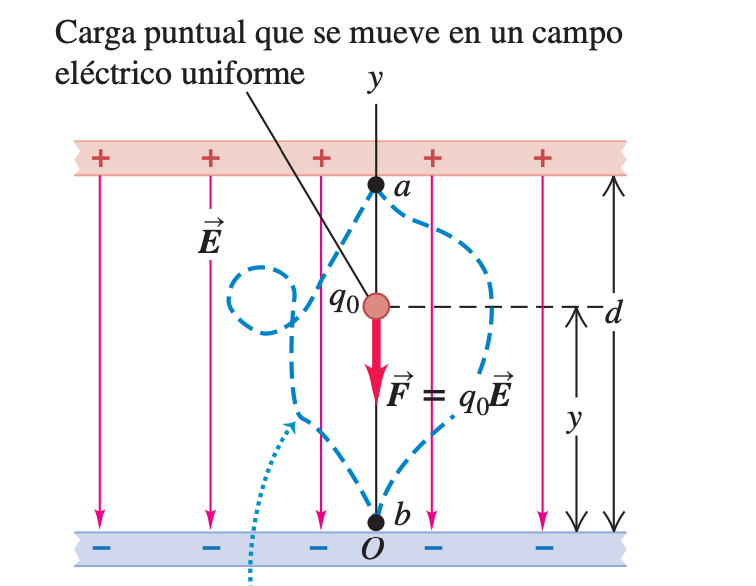
\includegraphics[scale=0.5]{fig/energia_potencial}
\caption{Trabajo realizado sobre una carga puntual que se mueve en un campo eléctrico uniforme. El trabajo realizado por la fuerza eléctrica es el mismo para cualquier trayectoria de $a$ a $b$: $W_{a\to b}=-\Delta U=q_0Ed$} 
\label{fig:energia_potencial}
\end{figure}

En la figura \ref{fig:energia_potencial} un par de placas metálicas paralelas con carga generan un campo eléctrico uniforme descendente y con magnitud $E$. El campo ejerce una fuerza hacia abajo con magnitud $F=q_0E$ sobre una carga de prueba positiva $q_0$. A medida que la carga se mueve hacia abajo una distancia $d$ del punto $a$ al punto $b$, la fuerza sobre la carga de prueba es constante e independiente de su localización. Por lo tanto, el trabajo realizado por el campo eléctrico es 

\begin{equation}\label{23.4}
W_{a\to b}=Fd=q_0Ed
\end{equation}

Este trabajo es positivo, toda vez que la fuerza está en la misma dirección que el desplazamiento neto de la carga de prueba. Este trabajo puede representarse con una función de \textbf{energía potencial} $U$, que para la fuerza eléctrica está dada por

\begin{equation}\label{23.5}
U=q_0Ey
\end{equation}

Cuando la carga de prueba se mueve de la altura $y_a$ a la altura $y_b$, el trabajo realizado sobre la carga por el campo está dado por

\begin{equation}\label{23.6}
W_{a\to b}=-\Delta U=-(U_b-U_a)=-(q_0Ey_b-q_0Ey_a)=q_0E(y_a-y_b)
\end{equation}

\subsection{Energía potencial entre dos cargas puntuales}
El concepto de energía potencial se puede aplicar a una carga puntual en \textit{cualquier} campo eléctrico generado por una distribución de carga estática. 
Cualquier distribución de carga se representa como un conjunto de cargas puntuales. Por consiguiente, es útil calcular el trabajo realizado sobre una carga de prueba $q_0$ que se mueve en el campo eléctrico ocasionado por una sola carga puntual estacionaria $q$.

En primer lugar se considerará un desplazamiento a lo largo de una línea radial, del punto $a$ al punto $b$. La fuerza sobre $q_0$ está dada por la ley de Coulomb, y su componente radial es

\begin{equation}\label{23.7}
F_r=\frac{1}{4\pi\epsilon_0}\frac{qq_0}{r^2}
\end{equation}

Si $q$ y $q_0$ tienen el mismo signo, la fuerza es de repulsión y $F_r$ es positiva; en caso contrario la fuerza es de atracción y $F_r$ es negativa. La fuerza \textit{no} es constante durante el desplazamiento, y se tiene que integrar para obtener el trabajo $W_{a\to b}$ que realiza esta fuerza sobre $q_0$ a medida que $q_0$ se mueve de $a$ a $b$

\begin{equation}\label{23.8}
W_{a\to b}=\int_{r_a}^{r_b}F_rdr=\int_{r_a}^{r_b}\frac{1}{4\pi\epsilon_0}\frac{qq_0}{r^2}dr=\frac{qq_0}{4\pi\epsilon_0}\left(\frac{1}{r_a}-\frac{1}{r_b}\right)
\end{equation}

El trabajo es el mismo para todas las trayectorias posibles entre $a$ y $b$. La fuerza sobre $q_0$ es \textit{conservativa}.\\
Se ve que las ecuaciones \ref{23.2} y \ref{23.8} son cosistentes si se define $qq_0/4\pi\epsilon_0r_a$ como la energia potencial $U_a$ cuando $q_0$ está en el punto $a$, a una distancia $r_a$ de $q$, y se define $qq_0/4\pi\epsilon_0r_b$ como la energía potencial $U_b$ cuando $q_0$ está en el punto $b$, a una distancia $r_b$ de $q$. De esta forma, la energía potencial $U$ cuando la carga de prueba $q_0$ está a cualquier distancia $r$ de la carga $q$ es

\begin{equation}\label{23.9.e_potencial}\marginnote{E. potencial eléctrica de dos cargas $q$ y $q_0$}
\boxed{U=\frac{1}{4\pi\epsilon_0}\frac{qq_0}{r}}
\end{equation}

\textbf{Obervación:} De las ecuaciones \ref{23.9.e_potencial} y \ref{23.7} notamos que tienen similitud. La energía potencial $U$ es proporcional a $1/r$, mientras que la componente de la fuerza $F_r$ es proporcional a $1/r^2$.\\
La energía potencial siempre se define en relación con algún punto de referencia donde $U=0$. En la ecuación \ref{23.9.e_potencial}, $U$ es igual a cero cuando $q$ y $q_0$ están infinitamente alejadas y $r=\infty$. Por lo tanto, \textbf{$U$ representa el trabajo que realizaría el campo de $q$ sobre la carga de prueba $q_0$ si esta última se desplazara de una distancia inicial $r$ al infinito}. La energía potencial $U$ es una propiedad \textit{compartida} de las dos cargas $q$ y $q_0$; es una consecuencia de la \textit{interacción} entre dos cuerpos.

La ley de Gauss dice que el campo eléctrico fuera de cualquier distribución de carga esféricamente simétrica es la misma que habría si toda la carga estuviera en el centro.

\subsection{Energía potencial eléctrica con varias cargas putuales}

\begin{figure}[h]
\centering
\caption{La energía potencial asociada con la carga $q_0$ en el punto a depende de las otras cargas $q_1, q_2$ y $q_3$ y de sus distancias $r_1, r_2$ y $r_3$ desde el punto $a$.}
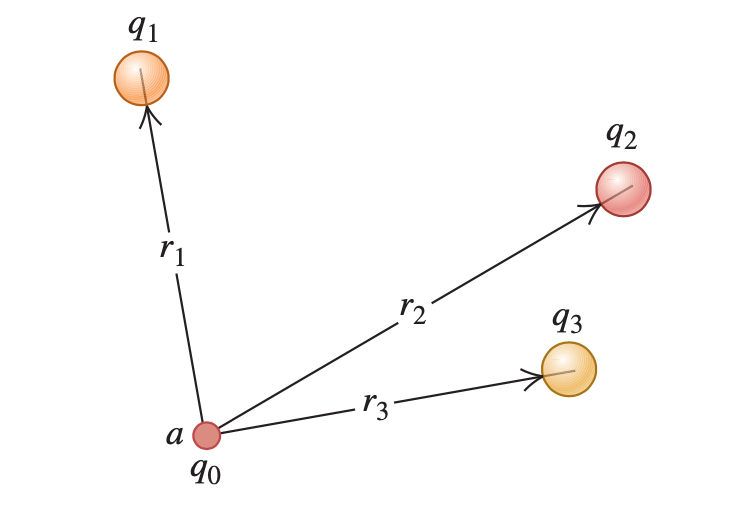
\includegraphics[scale=0.4]{fig/e_potencial_varias}
\label{fig:e_potencial_varias}
\end{figure}

Suponga que el campo eléctrico $\vec{E}$ en el que se desplaza la carga $q_0$ se debe a varias cargas puntuales $q_1, q_2, q_3$, . . . a distancias $r_1, r_2, r_3$, . . . de $q_0$. . El campo eléctrico total en cada punto es la \textit{suma vectorial} de los campos debidos a las cargas individuales, y el trabajo total realizado sobre $q_0$ durante cualquier desplazamiento es la suma de las contribuciones de las cargas individuales. De la ecuación \ref{23.9.e_potencial} se concluye que la energía potencial asociada con la carga de prueba $q_0$ en el punto a en la figura \ref{fig:e_potencial_varias} es la suma \textit{algebraica} (no la suma vectorial).

\begin{equation}\label{23.10}\marginnote{Carga puntual $q_0$ y conjunto de cargas $q_i$}
\boxed{U=\frac{q_0}{4\pi\epsilon_0}\left(\frac{q_1}{r_1}+\frac{q_2}{r_2}+\frac{q_3}{r_3}+\cdots \right)=\frac{q_0}{4\pi\epsilon_0}\sum_{i}\frac{q_i}{r_i}}
\end{equation}

El trabajo efectuado sobre la carga $q_0$ cuando se desplaza de $a$ a $b$ a lo largo de cualquier trayectoria es igual a la diferencia $U_a-U_b$ entre las energías potenciales cuando $q_0$ está en $a$ y en $b$.

Se puede representar \textit{cualquier} distribución de carga como un conjunto de cargas puntuales, por lo que la ecuación \ref{23.10} muestra que \textbf{para todo campo eléctrico debido a una distribución de carga estática, la fuerza ejercida por ese campo es conservativa.}

Las ecuaciones \ref{23.9.e_potencial} y \ref{23.10} definen que $U$ es igual a cero cuando todas las distancias $r_1, r_2, . . .$ son infinitas, es decir, cuando la carga de prueba $q_0$ está muy lejos de todas las cargas que producen el campo.

\subsubsection{Interpretación de la energía potencial eléctrica}
Definimos la energía potencial eléctrica en términos del trabajo realizado por el campo eléctrico sobre una partícula con carga que se mueve en el campo. Cuando una partícula se desplaza del punto $a$ al punto $b$, el trabajo que realiza sobre ella el campo eléctrico es $W_{a\to b}=U_a-U_b$. Por lo tanto, la diferencia de energía potencial $U_a-U_b$ es igual al \textit{trabajo que efectúa la fuerza eléctrica cuando la partícula se desplaza de $a$ a $b$}. Cuando $U_a$ es mayor que $U_b$ el campo realiza trabajo positivo sobre la partícula conforme “cae” de un punto de mayor energía potencial ($a$) a otro con menor energía potencial ($b$).

Un punto de vista alternativo pero equivalente es considerar cuánto trabajo se hubiera tenido que hacer para “subir” la partícula desde un punto $b$, en el que la energía potencial es $U_b$, hasta un punto $a$ en el que la energía potencial tiene un valor mayor $U_a$ (por ejemplo, al empujar dos cargas positivas para acercarlas). Para mover la partícula lentamente (de manera que no se le imparta ninguna energía cinética), es necesario ejercer una fuerza externa adicional $F_{ext}$ que es igual y opuesta a la fuerza del campo eléctrico y realiza un trabajo positivo. La diferencia de energía potencial $U_a-U_b$ se define entonces como el trabajo que debe efectuar una fuerza externa para desplazar la partícula lentamente desde $b$ hasta $a$ en contra de la fuerza eléctrica.

\section{Potencial eléctrico}
El \textbf{potencial} es \textit{la energía potencial por unidad de carga}. Se define el potencial $V$ en cualquier punto en el campo eléctrico como la energía potencial $U$ \textit{por unidad de carga} asociada con una carga de prueba $q_0$ en ese punto:

\begin{equation}\label{23.12}
V=\frac{U}{q_0} \quad\text{o bien, }\quad   U=q_0V
\end{equation}

La unidad del SI para el potencial es el \textbf{volt} (1 V):

\begin{equation*}
1\, \text{V}=1\, \text{J/C}
\end{equation*}

Dividiendo la ecuación \ref{23.2} entre $q_0$:

\begin{equation}\label{23.13}
\frac{W_{a\to b}}{q_0}=-\frac{\Delta U}{q_0}=-\left(\frac{U_b}{q_0}-\frac{U_a}{q_0}\right)=-(V_b-V_a)=V_a-V_b
\end{equation}

$V_a$ y $V_b$ se denominan el \textit{potencial en el punto a} y \textit{potencial en el punto b}, respectivamente. De este modo, el trabajo realizado por unidad de carga por la fuerza eléctrica cuando un cuerpo con carga se desplaza de $a$ a $b$ es igual al potencial en $a$ menos el potencial en $b$.

La diferencia $V_a-V_b$ se llama \textit{potencial de $a$ con respecto a $b$}; en ocasiones esa diferencia se abrevia como $V_{ab}=V_a-V_b$. En los circuitos eléctricos, a diferencia de potencial entre dos puntos con frecuencia se denomina \textbf{voltaje}. Así, la ecuación \ref{23.13} establece: \textbf{$V_{ab}$, el potencial de $a$ con respecto a $b$, es igual al trabajo realizado por la fuerza eléctrica cuando una UNIDAD de carga se desplaza de $a$ a $b$}. Otra interpretación válida tambien es \textbf{$V_{ab}$, el potencial de $a$ con respecto a $b$, es igual al trabajo que debe efectuarse para desplazar con lentitud una UNIDAD de carga de b a a contra la fuerza eléctrica}.

\subsection{Cálculo del potencial eléctrico}
Para encontrar el potencial $V$ debido a una sola carga puntual $q$, se divide la ecuación 	\ref{23.9.e_potencial} entre $q_0$:

\begin{equation}\label{23.14}\marginnote{Potencial debido a una carga puntual}
\boxed{V=\frac{U}{q_0}=\frac{1}{4\pi\epsilon_0}\frac{q}{r}}
\end{equation}

El potencial, como el campo eléctrico, es independiente de la carga de prueba $q_0$ que se utiliza para definirlo.

Para encontrar el potencial debido a un conjunto de cargas puntuales, se divide la ecuación \ref{23.10} entre $q_0$:

\begin{equation}\label{23.15}\marginnote{Potencial debido a un conjunto de cargas puntuales}
\boxed{V=\frac{U}{q_0}=\frac{1}{4\pi\epsilon_0}\sum_i\frac{q_i}{r_i}}
\end{equation}

Cuando se tiene una distribución continua de carga a lo largo de una línea, sobre una superficie o a través de un volumen, se divide la carga en elementos $dq$ y la suma en la ecuación \ref{23.15} se convierte en integral:

\begin{equation}\label{23.16}\marginnote{Potencial debido a un distribución contínua de carga}
\boxed{V=\frac{1}{4\pi\epsilon_0}\int\frac{dq}{r}}
\end{equation}

donde $r$ es la distancia que hay entre el elemento con carga $dq$ y el punto del campo donde se desea obtener $V$

\textbf{Observación}: El \textit{potencial} eléctrico en cierto punto es la energía potencial que estaría asociada a una carga \textit{unitaria} colocada en ese punto. Asimismo, hay que recordar que no tiene que haber una carga en un punto dado para que ahí exista un p tencial $V$.

\subsection{Obtención del potencial eléctrico a partir del campo eléctrico}
La fuerza $\vec{F}$ sobre una carga de prueba $q_0$ se escribe como $\vec{F}=q_0\vec{E}$ por lo que, según la ecuación \ref{23.1}, el trabajo realizado por la fuerza eléctrica conforme la carga de prueba se desplaza de $a$ a $b$ está dado por: 

\begin{equation*}
W_{a\to b}=\int_a^b\vec{F}\cdot d\vec{l}=\int_a^bq_0\vec{E\cdot d\vec{l}}
\end{equation*}

Si se divide entre $q_0$ y se compara el resultado con la ecuación \ref{23.13}, se encuentra que

\begin{equation}\label{23.17}\marginnote{Diferencial de potencial como integral de $\vec{E}$}
\boxed{V_a-V_b=\int_a^b\vec{E}\cdot d\vec{l}=\int_a^bE\cos\phi dl}
\end{equation}

El valor de $V_a-V_b$ es independiente de la trayectoria tomada de $a$ a $b$, del mismo modo en que el valor de $W_{a\to b}$ es independiente de la trayectoria. Para encontrar la ecuación \ref{23.17} hay que recordar que $\vec{E}$ es la fuerza eléctrica por unidad de carga sobre una carga de prueba.

La regla general, válida para \textit{cualquier} campo eléctrico, es la siguiente: desplazarse \textit{en} la dirección de $\vec{E}$ significa hacerlo en la dirección de $V$ \textit{decreciente}, y desplazarse \textit{contra de} la dirección de $\vec{E}$ signifca moverse en la dirección de $\vec{E}$ \textit{creciente}.

Observe que la ecuación \ref{23.17} se puede escribir como 

\begin{equation}\label{23.18}
V_a-V_b=-\int_b^{a}\vec{E}\cdot d\vec{l}
\end{equation}

La ecuación \ref{23.18} se puede interpretar de la siguiente manera: Para mover una unidad de carga lentamente en contra de la fuerza eléctrica, se debe aplicar una fuerza externa por unidad de carga igual a $-\vec{E}$, igual y opuesta a la fuerza eléctrica por unidad de carga $\vec{E}$.

\section{Cálculo del potencial eléctrico}
Cuando se calcula el potencial debido a una distribución de carga, por lo general se sigue una de dos rutas posibles. Si se conoce la distribución de carga se emplea la ecuación \ref{23.15} o la \ref{23.16}. O si se conoce el modo en que el campo eléctrico depende de la posición, se usa la ecuación \ref{23.17} estableciendo que el potencial es igual a cero en algún lugar conveniente.

\section{Superficies equipotenciales}
Una \textbf{superficie equipotencial} es una superficie tridimensional sobre la que el \textit{potencial eléctrico} $V$ es el mismo en todos los puntos. Si una carga de prueba $q_0$ se desplaza de un punto a otro sobre tal superficie, la energía potencial \textit{eléctrica} $q_0V$ permanece constante. Ningún punto puede estar en dos potenciales diferentes, por lo que las superficies equipotenciales para distintos potenciales nunca se tocan o intersecan.

\subsection{Superficies equipotenciales y líneas de campo}
Como la energía potencial no cambia a medida que una carga de prueba se traslada sobre una superficie equipotencial, el campo eléctrico no realiza trabajo sobre esa carga. De ello se deriva que $\vec{E}$ debe ser perpendicular a la superficie en cada punto, de manera que la fuerza eléctrica $q_0\vec{E}$ siempre es perpendicular al desplazamiento de una carga que se mueva sobre la superficie. \textbf{Las líneas de campo y las superficies equipotenciales siempre son perpendiculares entre sí}.

\textbf{Obervación}: En una superficie equipotencial dada, el potencial $V$ tiene el mismo valor en todos los puntos. Sin embargo, en general la magnitud del campo eléctrico $\vec{E}$ \textit{no} es la misma en todos los puntos sobre una superficie equipotencial.

\subsection{Equipotenciales y conductores}
\textbf{Cuando todas las cargas están en reposo, la superficie de un conductor siempre es una superficie equipotencial}. Como el campo eléctrico $\vec{E}$ siempre es perpendicular a una superficie equipotencial, el enunciado se puede demostrar si se prueba que \textbf{cuando todas las cargas están en reposo, el campo eléctrico justo afuera de un conductor debe ser perpendicular a la superficie en cada punto}. Se sabe que $\vec{E}=0$ en todos los lugares del interior del conductor; de otro modo, las cargas se moverían. $\vec{E}$ es perpendicular a la superficie en cada punto.

\section{Gradiente de potencial}
En la ecuación \ref{23.17}, $V_a-V_b$ es el potencial de $a$ con respecto de $b$, es decir, el cambio de potencial encontrado en un despalzamiento de $b$ a $a$. Esto es 

\begin{equation*}
V_a-V_b=\int_b^adV=-\int	_a^bdV
\end{equation*}

donde $dV$ es el cambio infinitesimal del potencial que acompaña un elemento infinitesimal $d\vec{l}$ de la trayectoria de $b$ a $a$. Comparando con la ecuación \ref{23.17} se tiene

\begin{equation*}
-\int_a^bdV=\int_a^b\vec{E}\cdot d\vec{l}
\end{equation*}

Estas dos integrales deben ser iguales para \textit{cualquier} par de límites $a$ y $b$, y para que esto se cumpla los \textit{integrados} deben ser iguales. Por lo tanto, para cualquier desplazamiento infinitesimal $$-dV=\vec{E}\cdot d\vec{l}$$

Las componentes de $\vec{E}$ se relacionan con las derivadas correspondientes de $V$ de la siguiente forma

\begin{equation}\label{23.19}\marginnote{Componentes de $\vec{E}$ en términos de $V$}
\boxed{E_x=-\frac{\partial V}{\partial x} \quad E_y=-\frac{\partial V}{\partial y} \quad E_z=-\frac{\partial V}{\partial z}}
\end{equation}

En términos de vectores unitarios, $\vec{E}$ se escribe como

\begin{equation}\label{23.20}\marginnote{$\vec{E}$ en términos de $V$}
\boxed{\vec{E}=-\left(\hat{i}\frac{\partial V}{\partial x}+\hat{j}\frac{\partial V}{\partial y}+\hat{k}\frac{\partial V}{\partial z}\right)}
\end{equation}

O en forma equivalente

\begin{equation}\label{23.22}
\vec{E}=-\vec{\nabla} V
\end{equation}

En cada punto, el gradiente de potencial señala en la dirección en que $V$ se \textit{incrementa} con más rapidez con un cambio de posición. De esta forma, en cada punto la dirección de $\vec{E}$ es la dirección en que $V$ \textit{disminuye} más rápido y siempre es perpendicular a la superficie equipotencial que pasa a través del punto.

Si $\vec{E}$ es radial con respecto a un punto o un eje, y $r$ es la distancia del punto o eje, la relación correspondiente a las ecuaciones \ref{23.19} es

\begin{equation}\label{23.23}\marginnote{Campo eléctrico radial}
\boxed{E_r=-\frac{\partial V}{\partial r}}
\end{equation}














































\chapter{Capacitancia y dieléctricos}
Un capacitor es un dispositivo que almacena energía potencial \textit{eléctrica} y carga eléctrica. Para hacerlo, basta aislar dos conductores uno del otro. Para almacenar energía en este dispositivo hay que transferir carga de un conductor al otro, de manera que uno tenga carga negativa y en el otro haya una cantidad igual de carga positiva. Debe realizarse trabajo para trasladar las cargas a través de la diferencia de potencial resultante entre los conductores, y el trabajo efectuado se almacena como energía potencial eléctrica.

Para un capacitor en particular, la razón entre la carga de cada conductor y la diferencia de potencial entre los conductores es una constante llamada \textit{capacitancia} \textbf{...}

\section{Capacitores y capacitancia}
Dos conductores separados por un aislante (o vacío) constituyen un \textbf{capacitor}. En la mayoría de las aplicaciones prácticas, cada conductor tiene inicialmente una carga neta cero, y los electrones son transferidos de un conductor al otro; a esta acción se le denomina \textit{cargar} el capacitor. Entonces, los dos conductores tienen cargas de igual magnitud y signo contrario, y la carga \textit{neta} en el capacitor en su conjunto permanece igual a cero. Cuando se dice que un capacitor tiene carga $Q$, o que una carga $Q$ está \textit{almacenada} en el capacitor, significa que el conductor con el potencial más elevado tiene carga $+Q$ y el conductor con el potencial más bajo tiene carga $-Q$ (si se supone que $Q$ es positiva). En los diagramas de circuito, un capacitor se representa con cualquiera de estos símbolos:

\begin{figure}[h]
\centering
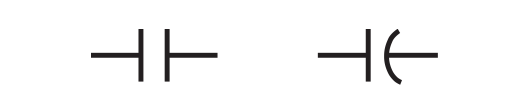
\includegraphics[scale=0.4]{fig/capacitor}
\end{figure}

En cada uno de estos símbolos, las líneas verticales (rectas o curvas) representan los conductores, y las líneas horizontales representan los alambres conectados a uno y otro conductor. Una manera común de cargar un capacitor es conectar estos dos alambres a las terminales opuestas de una batería. Una vez establecidas las cargas $Q$ y $-Q$ en los conductores, se desconecta la batería. Esto da una \textit{diferencia de potencial} fija $V_{ab}$ entre los conductores (el potencial del conductor con carga positiva $a$ con respecto al potencial del conductor con carga negativa $b$), que es exactamente igual al voltaje de la batería.

El campo eléctrico en cualquier punto de la región entre los conductores es proporcional a la magnitud $Q$ de carga en cada conductor. Por lo tanto, la diferencia de potencial $V_{ab}$ entre los conductores también es proporcional a $Q$. La \textit{razón} entre la carga y la diferencia de potencial no cambia. Esta razón se llama \textbf{capacitancia} $C$ del capacitor:

\begin{equation}\label{24.1}\marginnote{Definición de capacitancia}
\boxed{C=\frac{Q}{V_{ab}}}
\end{equation}

La unidad del SI para la capacitancia es el \textbf{farad} (1\, F)

Cuanto mayor es la capacitancia $C$ de un capacitor, mayor será la magnitud $Q$ de la carga en el conductor de cierta diferencia de potencial dada $V_{ab}$, y, por lo tanto, mayor será la cantidad de energía almacenada. \textit{La capacitancia es una medida de la aptitud (capacidad) de un capacitor para almacenar energía}. El valor de la capacitancia sólo depende de las formas y los tamaños de los conductores, así como de la naturaleza del material aislante que hay entre ellos. 

\subsection{Cálculo de capacitancia: capacitores con vacío}
Se considerarán \textit{capacitores con vacío}; es decir, se supondrá que los conductores que constituyen el capacitor están separados por un espacio vacío.

La forma más sencilla de un capacitor consiste en dos placas conductoras paralelas, cada una con área $A$, separadas por una distancia $d$ que es pequeña en comparación con sus dimensiones (figura \ref{fig:cap-1}).

\begin{figure}[t]
\centering
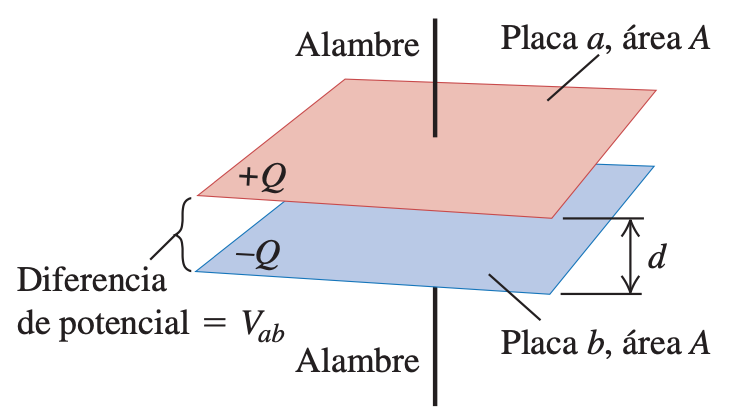
\includegraphics[scale=0.4]{fig/cap-placas-paralelas-1}
\caption{Arreglo de las placas del capacitor}
\label{fig:cap-1}
\end{figure}

\begin{figure}[t]
\centering
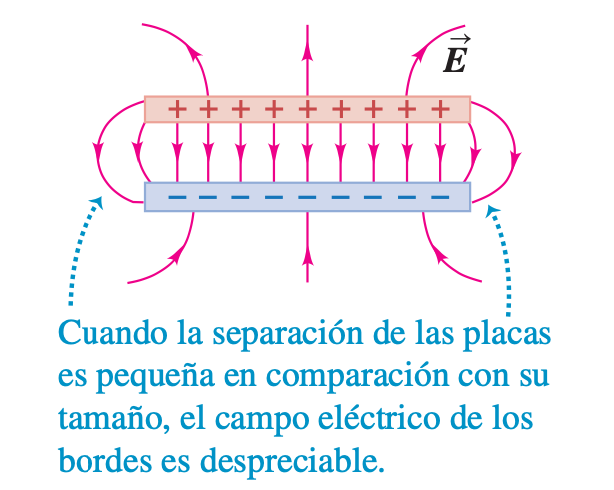
\includegraphics[scale=0.4]{fig/cap-placas-paralelas-2}
\caption{Vista lateral del campo eléctrico $\vec{E}$}
\label{fig:cap-2}
\end{figure}

Cuando las placas tienen carga, el campo eléctrico está localizado casi por completo en la región entre las placas (figura \ref{fig:cap-2}), el campo entre esas placas es esencialmente uniforme, y las cargas en las placas se distribuyen de manera uniforme en sus superficies opuestas. Este arreglo recibe el nombre de \textbf{capacitor de placas paralelas}.

Haciendo los cálculos, se sabe que, para este arreglo, la magnitud del cámpo eléctrico está dada por $E=\sigma/\epsilon_0$, donde $\sigma$ es la magnitud de la densidad superficial de carga en cada placa, es decir, $\sigma=Q/A$, por lo que se puede expresar como

\begin{equation*}
E=\frac{\sigma}{\epsilon_0}=\frac{Q}{\epsilon_0A}
\end{equation*}

El campo es uniforme y la distancia entre las placas es $d$, por lo que la diferencia de potencial (voltaje) es

\begin{equation*}
V_{ab}=Ed=\frac{1}{\epsilon_0}\frac{Qd}{A}
\end{equation*}

A partir de esto se observa que la capacitancia $C$ de un capacitor de placas paralelas con vacío es

\begin{equation}\label{24.2}\marginnote{Capacitancia de un capacitor de placas paralelas con vacío}
\boxed{C=\frac{Q}{V_{ab}}=\epsilon_0\frac{A}{d}}
\end{equation}

Notar que la capacitancia sólo depende de la geometría del capacitor. Cuando hay materia entre las placas, sus propiedades afectan la capacitancia.

\section{Capacitores en serie y en paralelo}
\subsection{Capacitores en serie}

\begin{figure}[h]
\centering
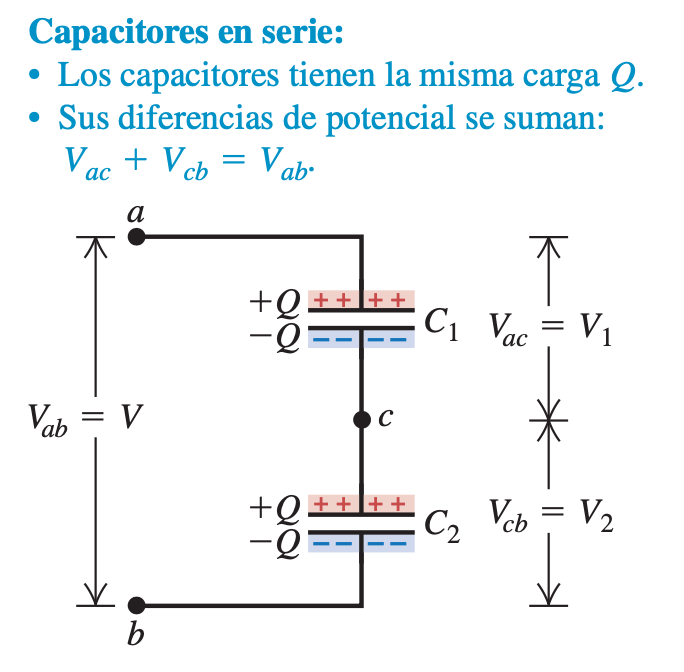
\includegraphics[scale=0.4]{fig/cap-serie-1}
\caption{Dos capacitores en serie}
\label{fig:cap-serie-1}
\end{figure}

\begin{figure}[h]
\centering
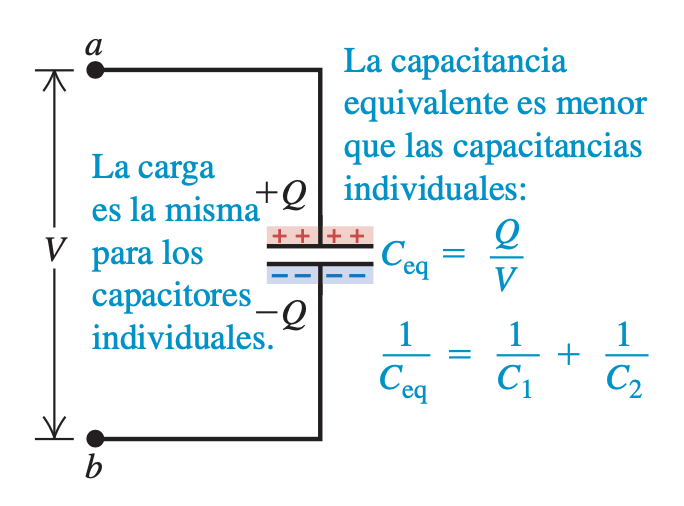
\includegraphics[scale=0.4]{fig/cap-serie-2}
\caption{El capacitor esquivalente único}
\label{fig:cap-serie-2}
\end{figure}

Se conectan en serie dos capacitores (uno en seguida del otro) mediante alambres conductores entre los puntos $a$ y $b$ (figura \ref{fig:cap-serie-1}).

\begin{equation}\label{24.5}\marginnote{Capacitores en serie}
\boxed{\frac{1}{C_{eq}}=\frac{1}{C_1}+\frac{1}{C_2}+\frac{1}{C_3}+\cdots}
\end{equation}

\begin{quote}
El recíproco de la capacitancia equivalente de una combinación en serie es igual a la suma de los recíprocos de las capacitancias individuales.
\end{quote}

\subsection{Capacitores en paralelo}
\begin{equation}\label{Capacitores en paralelo}\marginnote{Capacitores en paralelo}
\boxed{C_{eq}=C_1+C_2+C_3+\cdots}
\end{equation}

\begin{quote}
La capacitancia equivalente de una combinación en paralelo es igual a la suma de las capacitancias individuales.
\end{quote}

\section{Almacenamiento de energía en capacitores y energía de campo eléctrico}
La energía potencial eléctrica almacenada en un capacitor cargado es exactamente igual a la cantidad de trabajo requerido para cargarlo, es decir, para separar cargas opuestas y colocarlas en los diferentes conductores.

Suponga que cuando se carga el capacitor, la carga final es $Q$ y la diferencia de potencial final es $V$. Según la ecuación \ref{24.1}, estas cantidades están relacionadas de la siguiente forma $$V=\frac{Q}{C}$$

Sean $q$ y $v$ la carga y la diferencia de potencial, respectivamente, en una etapa intermedia del proceso de carga; entonces, $v=q/C$. En esta etapa, el trabajo $dW$ que se requiere para transferir un elemento adicional de carga $dq$ es $$dW=v\, dq=\frac{q\, dq}{C}$$

El trabajo total $W$ necesario para incrementar la carga $q$ del capacitor, de cero a un valor final $Q$, es

\begin{equation}\label{24.8}\marginnote{Trabajo para cargar el capacitor}
W=\int_0^WdW=\frac{1}{C}\int_0^Qq\, dq=\frac{Q^2}{2C}
\end{equation}

Si se define la energía potencial de un capacitor sin carga como igual a cero, entonces $W$ en la ecuación \ref{24.8} es igual a la energía potencial $U$ del capacitor con carga. La carga final almacenada es $Q=CV$, por lo que $U$ (que es igual a $W$) se expresa como

\begin{equation}\label{24.9}\marginnote{Energía almacenada en un capacitor}
\boxed{U=\frac{Q^2}{2C}=\frac{1}{2}CV^2=\frac{1}{2}QV}
\end{equation}

\subsection{Energía del campo eléctrico}
Debemos encontrar la energía por unidad de volumen en el espacio entre las placas paralelas de un capacitor con área $A$ y separación $d$. Ésta se denomina \textbf{densidad de energía} ($u$). De ecuación \ref{24.9}

\begin{equation}\label{24.10}
u=\frac{\frac{1}{2}CV^2}{Ad}
\end{equation}

De \ref{24.2} $C=\epsilon_0A/d$ y $V=Ed$. Reemplazando en \ref{24.10}

\begin{equation}\label{24.11}\marginnote{Densidad de energía eléctrica en vacío}
\boxed{u=\frac{1}{2}\epsilon_0E^2}
\end{equation}































\chapter{Corriente resistencia y fuerza electromotriz}
Una \textit{corriente eléctrica} consiste en cargas en movimiento de una región a otra. Cuando este desplazamiento tiene lugar en una trayectoria de conducción que forma una espira cerrada, la trayectoria recibe el nombre de \textit{circuito eléctrico}, los cuales, fundamentalmente, son un medio de transportar \textit{energía} de un lugar a otro.

\section{Corriente eléctrica}
Una \textbf{corriente eléctrica} es todo movimiento de carga de una región a otra.

\subsection{Dirección del flujo de corriente}
Definimos que la corriente, denotada por $I$, va en la dirección en la que hay un flujo de carga \textit{positiva}.  Por ello, las corrientes se describen como si consistieran por completo en un flujo de cargas positivas, aun en los casos en que se sabe que la corriente real se debe a electrones. Esta convención sobre la dirección del flujo de la corriente se llama \textbf{corriente convencional}. Aunque la dirección de la corriente convencional \textit{no} es necesariamente la misma en que se desplazan en realidad las partículas con carga. Definimos la corriente a través del área de sección transversal $A$ como la carga neta que fluye a través del área por unidad de tiempo. De esta forma, si una carga neta $dQ$ fluye a través de un área en el tiempo $dt$, la corriente $I$ a través del área es

\begin{equation}\label{25.1}\marginnote{Definición de corriente}
I=\frac{dQ}{dt}
\end{equation}

\textbf{La corriente no es un vector}.

La unidad del SI para la corriente es el \textbf{ampere}.

\subsection{Corriente, velocidad de deriva y densidad de corriente}

\begin{figure}[h]
\centering
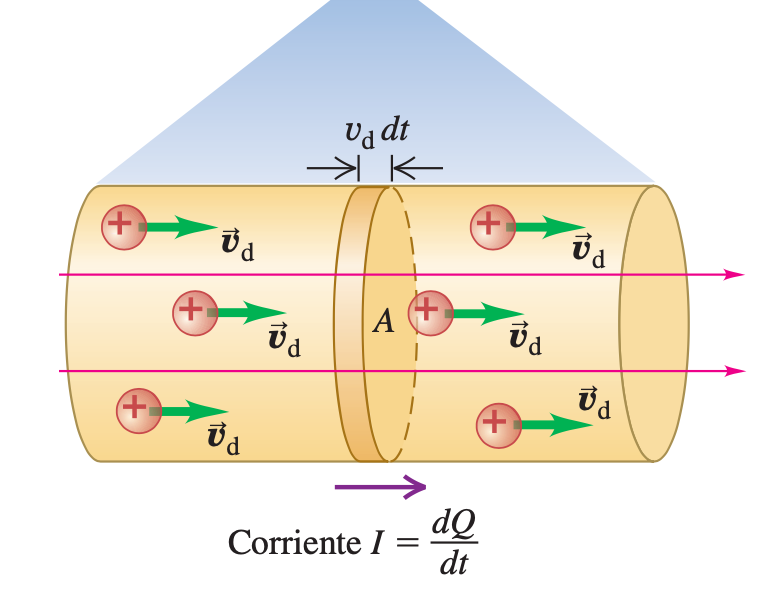
\includegraphics[scale=0.4]{fig/corriente}
\caption{La corriente $I$ es la tasa de transferencia de carga a través del área de la sección transversal $A$. La corriente va en la misma dirección de $\vec{E}$ sin que importe si las cargas en movimiento son positivas}
\label{fig:corriente}
\end{figure}

La corriente se puede expresar en términos de la velocidad de deriva de las cargas en movimiento. Consideremos la situación de la figura \ref{fig:corriente}. Suponga que hay $n$ partículas con carga en movimiento por unidad de volumen. Llamaremos $n$ a la concentración de partículas. Suponemos que todas las partículas se mueven con la misma velocidad de deriva con magnitud $v_d$. En un intervalo de tiempo $dt$, cada partícula se mueve una distancia $v_d\, dt$. Las partículas que fluyen hacia fuera del extremo derecho del cilindro sombreado cuya longitud es $v_d\, dt$ durante $dt$ son partículas que estuvieron dentro del cilindro al comienzo del intervalo $dt$. El volumen del cilindro es $Av_d\, dt$, y el número de partículas dentro es $nAv_d\, dt$. Si cada partícula tiene una carga $q$, la carga $dQ$ que fluye hacia fuera por el extremo del cilindro durante el tiempo $dt$ es

\begin{equation*}
dQ=q(nAv_d\, dt) = nqv_dA\, dt
\end{equation*}

y la corriente es

\begin{equation*}
I=\frac{dQ}{dt}=nqv_dA
\end{equation*}

La \textit{corriente por unidad de área de la sección transversal} se denomina \textbf{densidad de corriente} $J$:

\begin{equation*}
J=\frac{I}{A}=nqv_d
\end{equation*}

Si las cargas en movimiento son negativas en vez de positivas, la velocidad de deriva es opuesta a $\vec{E}$. Pero la corriente aún tiene la misma dirección que $\vec{E}$ en cada punto del conductor. Entonces, la corriente $I$ y la densidad de corriente $J$ no dependen del signo de la carga, por lo que en las expresiones anteriores para $I$ y $J$, la carga $q$ se sustituye por su valor absoluto $|q|$:

\begin{equation}\label{25.2}\marginnote{Expresión general para la corriente}
\boxed{I=\frac{dQ}{dt}=n|q|v_dA}
\end{equation}

\begin{equation}\label{25.3}\marginnote{Expresión general para la densidad de corriente}
J=\frac{I}{A}=n|q|v_d
\end{equation}

Se puede definir además una densidad de corriente vectorial $\vec{J}$ que incluye la dirección de la velocidad de deriva:

\begin{equation}\label{25.4}\marginnote{Densidad de corriente vectorial}
\boxed{\vec{J}=nq\vec{v}_d}
\end{equation}

Es posible tener una corriente \textit{estacionaria}, es decir, constante en el tiempo, sólo si el material conductor forma una espira cerrada, llamada \textit{circuito completo}. En una situación estacionaria, la carga total en cada segmento del conductor es constante. Por lo tanto, la tasa de flujo de carga hacia fuera de un extremo de un segmento en cualquier instante es igual a la tasa de flujo de carga hacia dentro en el otro extremo del segmento, y \textit{la corriente es la misma en todas las secciones transversales del circuito}.

\section{Resistividad}
La \textbf{resistividad} $\rho$ de un material se define como la razón de las magnitudes del campo eléctrico y la densidad de corriente:

\begin{equation}\label{25.5}\marginnote{Definición de resistividad}
\boxed{\rho=\frac{E}{J}}
\end{equation}

Un conductor perfecto tendría una resistividad igual a cero; y un aislante perfecto tendría resistividad infinita.

El recíproco de la resistividad es la \textbf{conductividad}.

Un material que obedece razonablemente bien la ley de Ohm se llama conductor \textit{óhmico} o \textit{conductor lineal}. 

\section{Resistencia}

\begin{figure}[h]
\centering
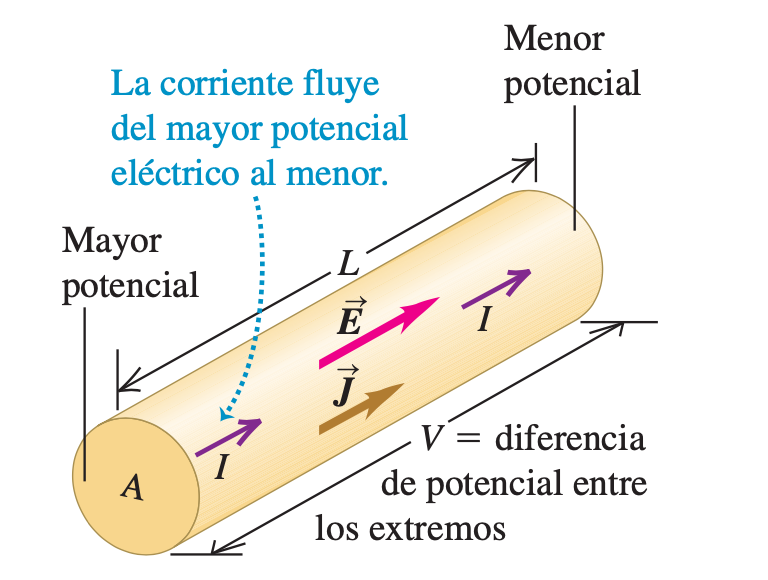
\includegraphics[scale=0.4]{fig/resistencia}
\caption{Conductor con sección transversal uniforme. La densidad de corriente es uniforme sobre cualquier sección transversal, y el campo eléctrico es constante en toda la longitud.}
\label{fig:resistencia}
\end{figure}

Para un conductor con resistividad $\rho$, con densidad de corriente $\vec{J}$ en un punto, el campo eléctrico $\vec{E}$ está dado por la ecuación \ref{25.5}

\begin{equation}\label{25.7}
 \vec{E}=\rho\vec{J}
\end{equation}

Suponga que nuestro conductor es un alambre con sección transversal uniforme de área $A$ y longitud $L$, como se ilustra en la figura \ref{fig:resistencia}. Sea $V$ la diferencia de potencial entre los extremos de mayor y menor potencial del conductor, de manera que $V$ es positiva. La \textit{dirección} de la corriente siempre va del extremo de mayor potencial al de menir potencial. Esto se debe a que en un conductor la corriente fluye en dirección de $\vec{E}$, sin importar el signo de las cargas en movimiento, y porque $\vec{E}$ apunta en la dirección del potencial eléctrico \textit{decreciente}.

También se puede relacionar el \textit{valor} de la corriente $I$ con la diferencia de potencial entre los extremos del conductor. Si las magnitudes de la densidad de corriente $\vec{J}$ y el campo eléctrico $\vec{E}$ son uniformes a través del conductor, la corriente total $I$ está dada por $I=JA$, y la diferencia de potencial $V$ entre los extremos es $V = EL$. Cuando se despejan $J$ y $E$, respectivamente, en estas ecuaciones y se sustituyen los resultados en la ecuación \ref{25.7}, se obtiene lo siguiente:

\begin{equation}\label{25.8}
\frac{V}{L}=\frac{\rho I}{A} \qquad \textup{o bien,}\qquad  V=\frac{\rho L}{A}I
\end{equation}

La razón de $V$ a $I$ para un conductor particular se llama \textbf{resistencia}, $R$:

\begin{equation}\label{25.9}
R=\frac{V}{I}
\end{equation}

Al comparar esta definición de $R$ con la ecuación \ref{25.8}, se observa que la resistencia $R$ de un conductor particular se relaciona con la resistividad $\rho$ del material mediante la ecuación

\begin{equation}\label{25.10}\marginnote{Relación entre la resistencia y la resistividad}
R=\frac{\rho L}{A}
\end{equation}

Si $\rho$ es constante, como en el caso de los materiales óhmicos, entonces también lo es $R$.

La ecuación 

\begin{equation}\label{25.11}\marginnote{Relación entre voltaje, corriente y resistencia}
\boxed{V=IR}
\end{equation}

suele identificarse con la \textit{ley de Ohm}. La relación \ref{25.11} define la resistencia $R$ para \textit{cualquier} conductor.

\section{Fuerza electromotriz y circuitos}
Para que un conductor tenga una corriente constante, debe ser parte de una trayectoria que forme una espira cerrada o \textbf{circuito completo}.

Para ver cómo mantener una corriente constante en un circuito completo, recordemos un hecho básico sobre la energía potencial eléctrica: si una carga $q$ recorre un circuito completo y regresa a su punto de partida, la energía potencial debe ser la misma al final y al principio del recorrido. Siempre hay una \textit{disminución} de la energía potencial cuando se desplazan cargas a través de un mate- rial conductor ordinario con resistencia. Así que debe haber una parte en el circuito en la que la energía potencial se \textit{incremente}.

\subsection{Fuerza electromotriz}
La influencia que hace que la corriente fluya del potencial menor al mayor (contrario a lo que ocurre en un conductor ordinario) se llama \textbf{fuerza electromotriz} (se abrevia \textbf{fem} $\varepsilon$).
Todo circuito completo con corriente constante debe incluir algún dispositivo que provea una fem. Tal dispositivo recibe el nombre de \textbf{fuente de fem}. Una fuente \textit{ideal} de fem mantiene una diferencia de potencial constante entre sus terminales, independiente de la corriente que pasa a través de ella. La fuerza electromotriz se define cuantitativamente como la magnitud de esta diferencia de potencial. 

\begin{equation}\label{25.13}\marginnote{Fuente ideal de fem}
V_{ab}=\varepsilon
\end{equation}

\section{Energía y potencia en circuitos eléctricos}

\begin{figure}[h]
\centering
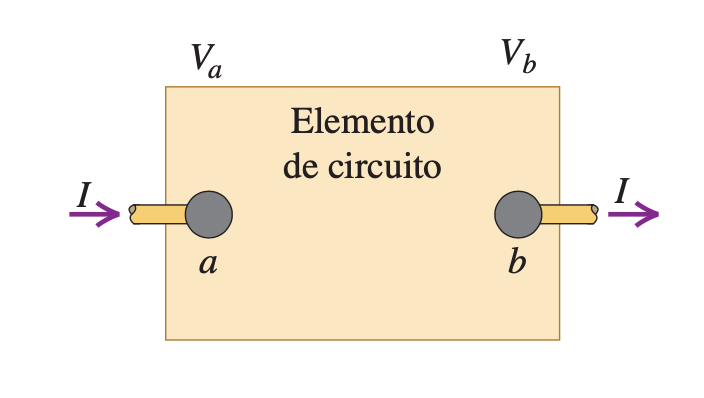
\includegraphics[scale=0.4]{fig/potencia}
\caption{La potencia de alimentación al elemento de circuito entre $a$ y $b$ es $P=(V_a-V_b)I=V_{ab}I$}
\label{fig:potencia}
\end{figure}

La caja de la figura \ref{fig:potencia} representa un elemento de circuito con diferencia de potencial $V_a-V_b=V_{ab}$ entre sus terminales y la corriente $I$ que pasa a través suyo en dirección de $a$ hacia $b$. Conforme la carga pasa por el elemento de circuito, el campo eléctrico realiza trabajo sobre la carga.

En los circuitos eléctricos es más frecuente que interese la \textit{rapidez} con la que la energía se proporciona a un elemento de circuito o se extrae de él. Si la corriente a través del elemento es $I$, entonces en un intervalo de tiempo $dt$ pasa una cantidad de carga $dQ=I\, dt$ a través del elemento. El cambio en la energía potencial para esta cantidad de carga es $V_{ab}\, dQ=V_{ab} I\, dt$.  Si esta expresión se divide entre $dt$, se obtiene la rapidez a la que se transfiere la energía hacia fuera o hacia dentro de circuito. La relación de transferencia de energía por unidad de tiempo es la \textit{potencia}, y se denota mediante $P$

\begin{equation}\label{25.17}\marginnote{Rapidez con la que se entrega energía a un elemento de circuito o se extrae de éste}
\boxed{P=V_{ab}I}
\end{equation}

\subsection{Potencia de una resistencia pura}
Si el elemento de circuito de la figura \ref{fig:potencia} es un resistor, la diferencia de potencial es $V_{ab}=IR$. De ecuación \ref{25.17}, la potencia eléctrica entregada al resistor por circuito es

\begin{equation}\label{25.18}\marginnote{Potencia entregada a un resistor}
P=V_{ab}I=I^2R=\frac{{V_{ab}}^2}{R}
\end{equation}















































\chapter{Circuitos de corriente directa}
\section{Resistores en serie y en paralelo}
Cuando se conectan en secuencia varios elementos de circuito, como resistores, baterías y motores con una sola trayectoria de corriente entre los puntos, se dice que están conectados \textbf{en serie}. Se dice que los resistores están conectados \textbf{en paralelo} entre los puntos $a$ y $b$ si cada resistor ofrece una trayectoria alternativa entre los puntos.

Para cualquier combinación de resistores siempre es posible encontrar un resistor \textit{único} que podría remplazar la combinación y dar como resultado la misma corriente y diferencia de potencial totales. La resistencia de este resistor único se llama \textbf{resistencia equivalente} de la combinación.

\subsection{Resistores en serie}
Si los resistores están en \textit{serie}, la corriente $I$ debe ser la misma en todos ellos (la corriente no “se gasta” cuando pasa a través de un circuito). Al aplicar $V=IR$ a cada resistor, se obtiene

\begin{equation*}
V_{ax}=IR_1 \qquad V_{xy}=IR_2 \qquad V_{yb}=IR_3
\end{equation*}

Las diferencias de potencial a través de cada resistor no necesitan ser las mismas (excepto para el caso especial en que las tres resistencias son iguales). La diferencia de potencial $V_{ab}$ a través de toda la combinación es la suma de estas diferencias de potencial individuales:

\begin{equation*}
V_{ab}=V_{ax}+V_{xy}+V_{yb}=I(R_1+R_2+R_3)
\end{equation*}

por lo que 

\begin{equation*}
\frac{V_{ab}}{I}=R_1+R_2+R_3
\end{equation*}

La razón $V_{ab}/I$ es, por definición, la resistencia equivalente $R_{eq}$, por tanto, generalizando, se tiene

\begin{equation}\label{26.1}\marginnote{Resistores en serie}
\boxed{R_{eq}=R_1+R_2+R_3+ \cdots}
\end{equation}

\begin{quote}
La resistencia equivalente de cualquier número de resistores en serie es igual a la suma de sus resistencias indivuduales.
\end{quote}

\subsection{Resistores en paralelo}
Si los resistores están en \textit{paralelo}, la corriente a través de cada resistor no necesita ser la misma, pero la diferencia de potencial entre las terminales de cada resistor debe ser la misma e igual a $V_{ab}$. De $I=V/R$

\begin{equation*}
I_1=\frac{V_{ab}}{R_1} \qquad I_2=\frac{V_{ab}}{R_2} \qquad I_3=\frac{V_{ab}}{R_3}
\end{equation*}

En general, la corriente es diferente a través de cada resistor. Como la carga no se acumula o escapa del punto $a$, la corriente total $I$ debe ser la suma de las tres corrientes en los resistores:

\begin{equation*}
I=I_1+I_2+I_3=V_{ab}\left(\frac{1}{R_1}+\frac{1}{R_2}+\frac{1}{R_3}\right)
\end{equation*}

Generalizando

\begin{equation}\label{26.2}\marginnote{Resistores en paralelo}
\frac{1}{R_{eq}}=\frac{1}{R_1}+\frac{1}{R_2}+\frac{1}{R_3}+\cdots
\end{equation}

\begin{quote}
Para cualquier número de resistores en paralelo, el \textit{recíproco} de la resistencia equivalente es igual a la suma de los recíprocos de sus resistencias individuales.
\end{quote}

\section{Reglas de Kirchhoff}
Una \textbf{unión} en un circuito es el punto en que se unen tres o más conductores. Las uniones también reciben el nombre de \textit{nodos} o \textit{puntos de derivación}. Una \textbf{espira} es cualquier trayectoria cerrada de conducción. Las reglas de Kirchhoff consisten en los dos siguientes enunciados:

\textbf{Regla de Kirchhoff de las uniones:} la suma algebraica de las corrientes en cualquier unión es igual a cero. Es decir,

\begin{equation}\label{26.5}\marginnote{Regla de las uniones, válida en cualquier unión}
\boxed{\sum I=0}
\end{equation}

\textbf{Regla de Kirchhoff de las espiras:} la suma algebraica de las diferencias de potencial en cualquier espira, incluso las asociadas con las fem y las de elementos con resistencia, debe ser igual a cero. Es decir,

\begin{equation}\label{26.6}\marginnote{Regla de las espiras, válida para cualquier espira cerrada}
\boxed{\sum V=0}
\end{equation}

La regla de las uniones se basa en la conservación de la carga eléctrica. La regla de las uniones se basa en la conservación de la carga eléctrica.

\section{Circuitos $R-C$}
\subsection{Carga de un capacitor}

\begin{figure}[h]
\centering
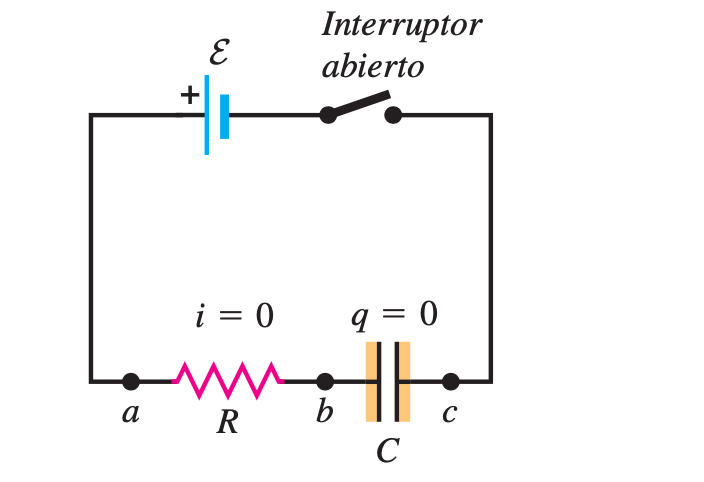
\includegraphics[scale=0.4]{fig/r-c-1}
\caption{Capacitor descargado al inicio. Cuando el interrupor se cierra, a medida que transcurre el tiempo, la carga en el capacitor se incrementa y la corriente disminuye}
\label{fig:r-c-1}
\end{figure}

Un circuito que tiene un resistor y un capacitor conectados en serie, se llama circuito $R-C$ (figura \ref{fig:r-c-1}). Se comienza con el capacitor descargado, después, en cierto momento inicial, $t=0$, se cierra el interruptor, lo que completa el circuito y permite que la corriente alrededor de la espira comience a cargar el capacitor.

Como el capacitor de la figura \ref{fig:r-c-1} al principio está descargado, la diferencia de potencial $v_{bc}$ a través suyo es igual a cero en $t=0$. Después de un periodo largo, el capacitor está cargado por completo, la corriente baja a cero y la diferencia de potencial $v_{ab}$ a través del resistor se vuelve cero. En ese momento aparece la totalidad de la fem $\varepsilon$ de la batería a través del capacitor y $v_{bc}=\varepsilon$. Las diferencias de potencial instantáneas $v_{ab}$ y $v_{bc}$ son

\begin{equation*}
v_{ab}=iR \qquad v_{bc}=\frac{q}{C}
\end{equation*}

Con la regla de Kirchhoff de las espiras, se obtiene

\begin{equation}\label{26.9}
\varepsilon -iR-\frac{q}{C}=0
\end{equation}

Despejando $i$ de la ecuación \ref{26.9}

\begin{equation}\label{26.10}
i=\frac{\varepsilon}{R}-\frac{q}{RC}
\end{equation}

Conforme la carga se incrementa, el término $q/RC$ se hace más grande y la carga del capacitor tiende a su valor final, al que llamaremos $Q_f$. La corriente disminuye y finalmente se vuelve cero. Cuando $i=0$, la ecuación \ref{26.10} da 

\begin{equation}\label{26.11}
\frac{\varepsilon}{R}=\frac{Q_f}{RC} \qquad Q_f=C\varepsilon
\end{equation}

Observe que la carga final $Q_f$ no depende de $R$.

Es posible obtener expresiones generales para la carga $q$ y la corriente $i$ como funciones del tiempo. De ecuación \ref{26.10}
\begin{equation*}
\frac{dq}{dt}=\frac{\varepsilon}{R}-\frac{q}{RC}=-\frac{1}{RC}(1-C\varepsilon)
\end{equation*}
\begin{equation*}
\frac{dq}{q-C\varepsilon}=-\frac{dt}{RC}
\end{equation*}
\begin{equation*}
\int_0^q\frac{dq'}{q'-C\varepsilon}=-\int_0^t\frac{dt'}{RC}
\end{equation*}
\begin{equation*}
\ln\left(\frac{q-C\varepsilon}{-C\varepsilon}\right)=-\frac{t}{RC}
\end{equation*}
\begin{equation*}
\frac{q-C\varepsilon}{-C\varepsilon}=e^{-t/RC}
\end{equation*}

\begin{equation}\label{26.12}\marginnote{Circuito $R-C$, capacitor en carga}
\boxed{q=C\varepsilon \left(1-e^{-t/RC}\right)=Q_f\left(1-e^{-t/RC}\right)}
\end{equation}

Derivando la carga con respecto al tiempo, se tiene

\begin{equation}\label{26.13}\marginnote{Circuito $R-C$, capacitor en carga}
\boxed{i=\frac{dq}{dt}=\frac{\varepsilon}{R}e^{-t/RC}=I_0e^{-t/RC}}
\end{equation}

\subsection{Descarga de un capacitor}

\begin{figure}[h]
\centering
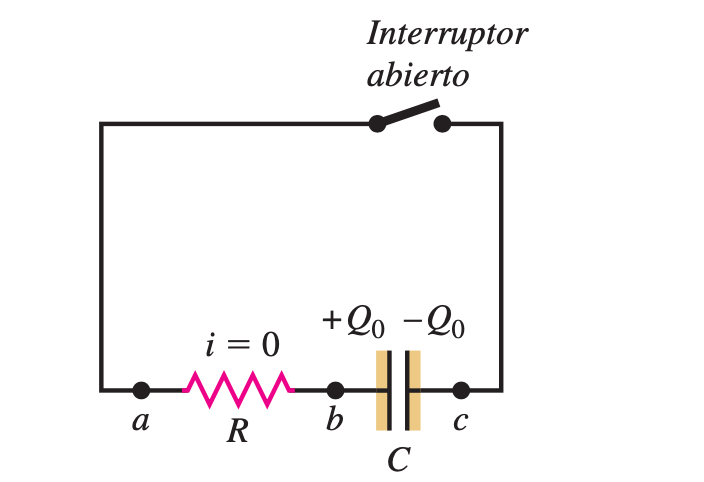
\includegraphics[scale=0.4]{fig/r-c-2}
\caption{Capacitor inicialmente cargado. Cuando se cierra el interruptor, tanto la carga en el capacitor como la corriente disminuyen con el tiempo.}
\label{fig:r-c-2}
\end{figure}

Ahora suponga que después de que el capacitor de la figura \ref{fig:r-c-2} ha adquirido una carga $Q_0$, se retira la batería del circuito $R-C$ y se conectan los puntos $a$ y $c$ a un interruptor abierto. Después se cierra el interruptor y en el mismo instante se reajusta el cronómetro a $t=0$; en ese momento, $q=Q_0$. Luego, el capacitor se descarga a través del resistor y su carga disminuye finalmente a cero. 

Haciendo un cálculo similar al anterior, considerando que en este caso $\varepsilon=0$ en la ecuación de malla, se tiene

\begin{equation}\label{26.16}\marginnote{Circuito $R-C$, capacitor en descarga}
\boxed{q=Q_0e^{-t/RC}}
\end{equation}
Derivando la carga con respecto al tiempo

\begin{equation}\label{26.17}\marginnote{Circuito $R-C$, capacitor en descarga}
\boxed{i=\frac{dq}{dt}=-\frac{Q_0}{RC}=e^{-t/RC}=I_0e^{-t/RC}}
\end{equation}

Mientras el capacitor se carga, la tasa instantánea a la que la batería entrega energía al circuito es $P=\varepsilon i$. La tasa instantánea a la que la energía eléctrica se disipa en el resistor es $i^2R$, y la tasa a que la energía se almacena en el capacitor es $i\, v_{bc}=iq/C$. Al multiplicar la ecuación \ref{26.9} por $i$ se obtiene:

\begin{equation}\label{26.18}
\varepsilon i=i^2R+\frac{iq}{C}
\end{equation}

Esto significa que de la potencia $\varepsilon i$ suministrada por la batería, una parte $(^i2R)$ se disipa en el resistor y otra parte $(iq/C)$ se almacena en el capacitor.

La energía \textit{total} suministrada por la batería durante la carga del capacitor es igual a la fem de la batería $\varepsilon$ multiplicada por el total de la carga $Q_f$, o $\varepsilon Q_f$. La energía total almacenada en el capacitor, según la ecuación \ref{24.9}, es $Q_f \varepsilon/2$. Así, \textit{exactamente} la mitad de la energía suministrada por la batería se almacena en el capacitor, y la otra mitad se disipa en el resistor. Este resultado también se puede verificar en detalle tomando la integral con respecto al tiempo de cada una de las cantidades de potencia en la ecuación \ref{26.18}.





































































\chapter{Fuentes de campo magnético}
\section{Campo de una carga en movimiento}
Comenzaremos con lo fundamental: el campo magnético de una sola carga puntual $q$ que se mueve con velocidad constante $\vec{v}$. Los experimentos demuestran que la magnitud de $\vec{B}$ es proporcional a $|q|$ y a $1/r^2$, pero su dirección \textit{no} es a lo largo de de la línea que va desde el punto de fuente al punto de campo. En vez de ello, $\vec{B}$ es perpendicular al plano que contiene esta línea y al vector velocidad, de la partícula, $\vec{v}$. Además, la magnitud $\vec{B}$ del campo también es proporcional a la rapidez $\vec{v}$ de la partícula y al seno del ángulo $\phi$. Así, la magnitud del campo magnético en el punto $P$ está dada por
\begin{equation}\label{28.1}
B=\frac{\mu_0}{4\pi}\frac{|q|v\sin\phi}{r^2}
\end{equation}
donde $\mu_0/4\pi$ es una constante de proporcionalidad.
En forma vectorial
\begin{equation}\marginnote{C. magnético de una carga puntual con velocidad constante}
\boxed{\vec{B}=\frac{\mu_0}{4\pi}\frac{q\vec{v}\times\hat{r}}{r^2}}
\end{equation}
\textbf{Nota}: Las partículas con carga que constituyen una corriente en un alambre aceleran en los puntos en que éste se dobla y la dirección de $\vec{v}$ cambia. Pero como la magnitud $v_d$ de la velocidad de deriva en un conductor por lo general es muy pequeña, la aceleración $v_d^2/r$ también lo es, por lo que pueden ignorarse los efectos de la aceleración.

La unidad en el SI de $B$ es un \textbf{tesla} [1T].

En unidades del SI, el valor numérico de $\mu_0$ es exactamente $4\pi\times 10^{-7}$
\section{Campo magnético de un elemento de corriente}
\textbf{Principio de superposición de campos magnéticos}:  El campo magnético total generado por varias cargas en movimiento es la suma vectorial de los campos generados por las cargas individuales.

\textit{Cálculo del campo magnético ocasionado por un segmento corto $d\vec{l}$ de un conductor que transporta corriente}:

El volumen del segmento es $A dl$, donde $A$ es el área de la sección transversal del conductor. Si hay $n$ partículas con carga en movimiento por unidad de volumen, cada una con una carga $q$, la carga total $dQ$ que se mueve en el segmento es $$dQ=nqAdl$$ Las cargas en movimiento en este segmento son equivalentes a una sola carga $dQ$
que viaja con una velocidad igual a la velocidad de \textit{deriva} $\vec{v}_d$. (Los campos magnéticos debidos a los movimientos al azar de las cargas, en promedio, se cancelarán en cada punto.) De ec. \ref{28.1}, la magnitud del campo resultante $d\vec{B}$ en cualquier punto $P$ es
\begin{equation}\label{28.5}
dB=\frac{\mu_0}{4\pi}\frac{|dQ|v_d\sin\phi}{r^2}=\frac{\mu_0}{4\pi}\frac{n|q|v_dAdl\sin\phi}{r^2}=\frac{\mu_o}{4\pi}\frac{Idl\sin\phi}{r^2}
\end{equation} 
porque de ec (25.2), $n|q|v_dA$ es igual a la corriente $I$ en el elemento.

En su forma vectorial
\begin{equation}\label{28.6}\marginnote{C. magnético de un elemento de corriente}
\boxed{d\vec{B}=\frac{\mu_0}{4\pi}\frac{Id\vec{l}\times\hat{r}}{r^2}}
\end{equation}
donde $d\vec{l}$ es un vector con longitus $dl$, en la misma dirección que la corriente del coductor.
 
Las ecuaciónes \ref{28.5} y \ref{28.6} constituyen la \textbf{ley de Biot y Savat}. Esta ley se utiliza para encontrar el campo magnético total $B$ debido a la corriente en un circuito completo en cualquier punto en el espacio.
\section{Campo magnético de un conductor que transporta corriente}
\begin{figure}[h]
\centering
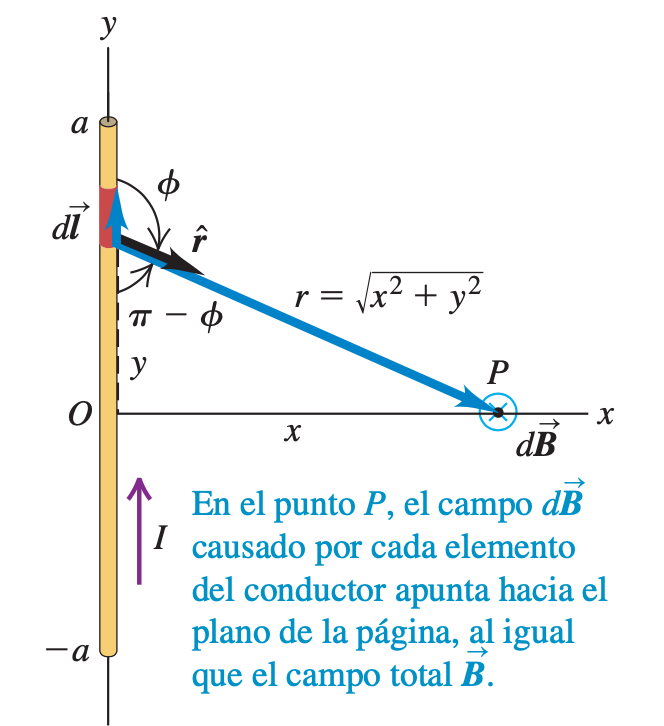
\includegraphics[scale=0.6]{fig/image1}
\caption{Campo magnético producido por un conductor recto portador de corriente de longitud infinita.}
\label{fig:28.5}
\end{figure}
Usando la ley de Biot y Savat, (\ref{28.6}), y haciendo los cálculos correspondientes, se tiene que $B$ debe tener la misma magnitud en todos los puntos de un círculo con centro en el conductor y que yace en un plano perpendicular a él, y la dirección de $B$ debe ser tangente a todo ese círculo. Así, 
\begin{equation}\label{28.9}\marginnote{C. magnético cerca de un conductor largo y recto portador de corriente}
\boxed{\vec{B}=\frac{\mu_0I}{2\pi r}\hat{\phi}}
\end{equation}
\textbf{Observaciones:}
\begin{enumerate}
\item Las líneas de campo magnético circundan la corriente que actúa como su fuente.
\item Las líneas del campo magnético forman espiras cerradas y \textit{nunca} tienen extremos, sin importar la forma del conductor portador de corriente que genera el campo. Ésta es una consecuencia de la ley de Gauss para el magnetismo, que plantea que el flujo magnético total a través de cualquier superficie cerrada siem- pre es igual a cero:
\begin{equation}\label{28.10}
\oint\vec{B}\cdot d\vec{A}=0
\end{equation}
Esto implica que no hay cargas magnéticas aisladas ni monopolos magnéticos. \textbf{Cualquier línea de campo magnético que entre a una superficie cerrada debe salir de ella}.
\end{enumerate}
\section{Fuerza entre alambres paralelos}
\begin{figure}[h]\label{fig2}
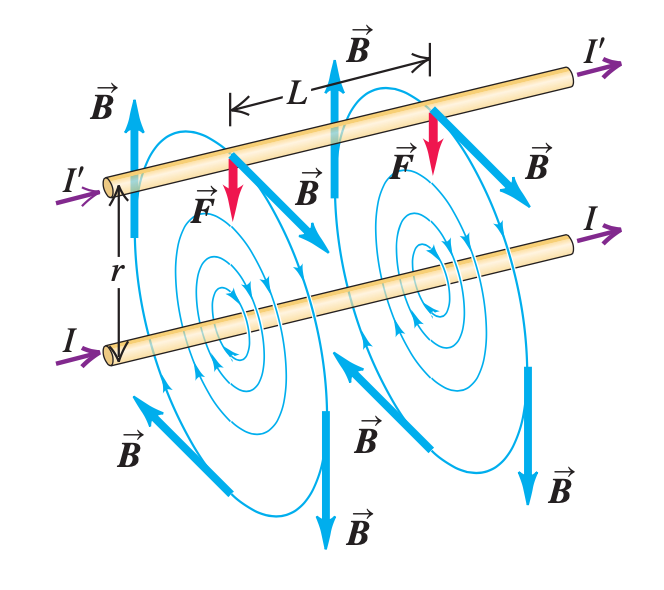
\includegraphics[scale=0.6]{fig/image2}
\centering
\end{figure}
De acuerdo con la ecuación \ref{28.9}, el conductor inferior produce un campo $\vec{B}$ que, en la posición del conductor de arriba, tiene una magnitud $$B=\frac{\mu_0I}{2\pi r}$$ De ecuación (27.19) la fuerza que ejerce este campo sobre una longitud $L$ del conductor superior es $\vec{F}=I' \vec{L}\times\vec{B}$,  donde el vector $\vec{L}$ está en dirección de la corriente $I'$ y tiene magnitud $L$. Como $\vec{B}$ es perpendicular a la longitud del conductor y, por lo tanto, a $\vec{L}$, la magnitud de esta fuerza es $$F=I'LB=\frac{\mu_oII'L}{2\pi r}$$ Luego, la \textit{fuerza por unidad de longitud}, $F/L$ está dada por
\begin{equation}\label{28.11}\marginnote{Magnitud de la fza. entre dos coductores largos, paralelos y portadores de
corriente}
\boxed{\frac{F}{L}=\frac{\mu_0II'}{2\pi r}}
\end{equation}
La aplicación de la regla de la mano derecha a $\vec{F}=I'\vec{L}\times\vec{B}$ indica que la fuerza sobre el conductor de arriba está dirigida hacia abajo.

\textbf{Observación}:
\begin{enumerate}
\item Dos conductores paralelos que transportan corrientes en el mismo sentido se atraen uno al otro.
\item Dos conductores paralelos que transportan corrientes en sentido opuestos se repelen entre sí.
\end{enumerate}
\section{Campo magnético de una espira circular de corriente}
\begin{figure}[h]
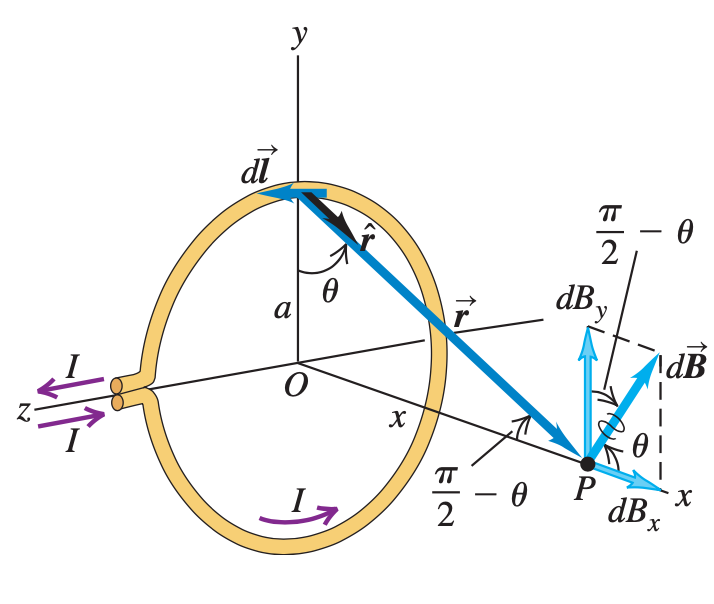
\includegraphics[scale=0.6]{fig/image3}
\centering
\caption{Alambre circular que transporta corriente}
\label{fig3}
\end{figure}
Para encontrar el campo magnético en el punto $P$ sobre el eje de la espira, se usa la ley de Biot y Savart, ecuación (\ref{28.5}) o (\ref{28.6}). De la figura \ref{fig3}, $d\vec{l}$ y $\vec{r}$ son perpendiculares, y la dirección del campo $d\vec{B}$ generado por este elemento $d\vec{l}$ en particular yace sobre el plano $xy$. La magnitud $dB$ del campo debido al elemento $d\vec{l}$ es
\begin{equation}\label{28.15}
\boxed{B_x=\frac{\mu_0Ia^2}{2(x^2+a^2)^{3/2}}}
\end{equation}
Si se cierran los dedos de la mano derecha alrededor de la espira en la dirección de la corriente, el pulgar derecho apunta en la dirección del campo.
\subsection{Campo magnético sobre el eje de una bobina}
Ahora suponga que en vez de una sola espira en la figura \ref{fig3}, se tiene una bobina que consiste en N espiras. Cada espira contribuye por igual al campo, y el total es N veces el campo producido por una sola espira:
\begin{equation}\label{28.16}
B_x=\frac{\mu_0NIa^2}{2(x^2+a^2)^{3/2}}
\end{equation}
En el centro de $N$ espiras circulares la magnitud del campo magnético vale
\begin{equation}\label{28.17}
\boxed{B_x=\frac{\mu_0Ia^2}{2a}}
\end{equation}
Conforme se avanza a lo largo del eje, la magnitud del campo disminuye.
\textbf{Observación}: Las ecuaciones (\ref{28.15}) y (\ref{28.16}) son válidas sólo sobre el \textit{eje} de una espira o bobina. No sobre otros puntos.


\section{Ley de Ampere}
\begin{equation}\label{28.20.ampere}\marginnote{Ley de Ampere}\footnote{Sólo válida si las corrientes son estables y si no están presentes materiales magnéticos o campos eléctricos que varíen con el tiempo.}
\boxed{\oint\vec{B}\cdot d\vec{l}=\mu_0I_{enc}}
\end{equation}
Hay una regla simple para determinar el signo de la corriente; Doble los dedos de su mano derecha alrededor de la trayectoria de integración en la dirección de esta última, es decir, la dirección que usa para evaluar $\oint\vec{B}\cdot d\vec{l}$. En esas condiciones, su pulgar derecho indica la dirección de la corriente positiva. Las corrientes que pasan a través de la trayectoria de integración en esta dirección son positivas; aquéllas en dirección opuesta son negativas. La ecuación (\ref{28.20.ampere}) de hecho es válida para conductores y trayectorias de \textbf{cualquier} forma.

\textbf{Observación}: Si $\oint\vec{B}\cdot d\vec{l}=0$, no necesariamente significa que $\vec{B}=0$
\subsection{Campo de un soleoide}
\begin{figure}[h]
\centering
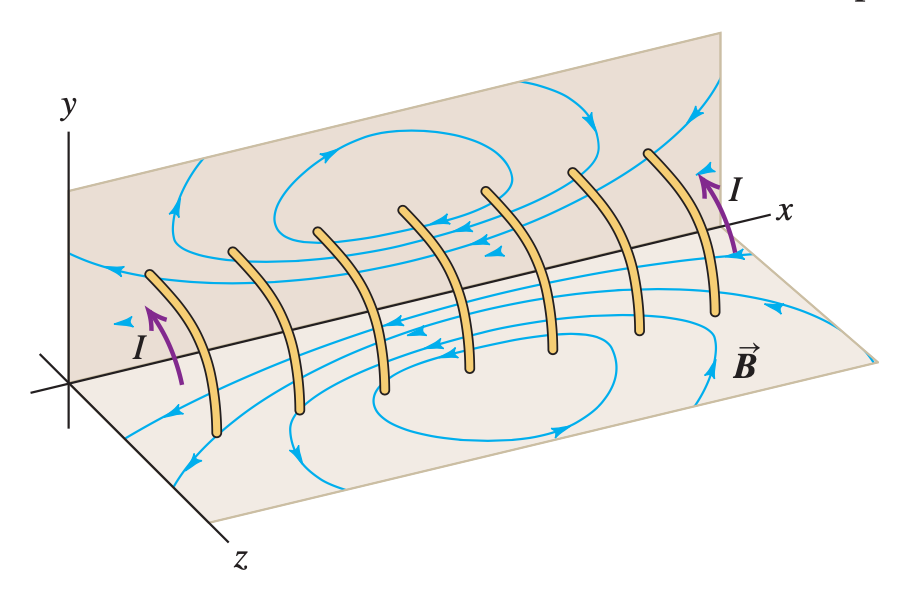
\includegraphics[scale=0.4]{fig/solenoide1}
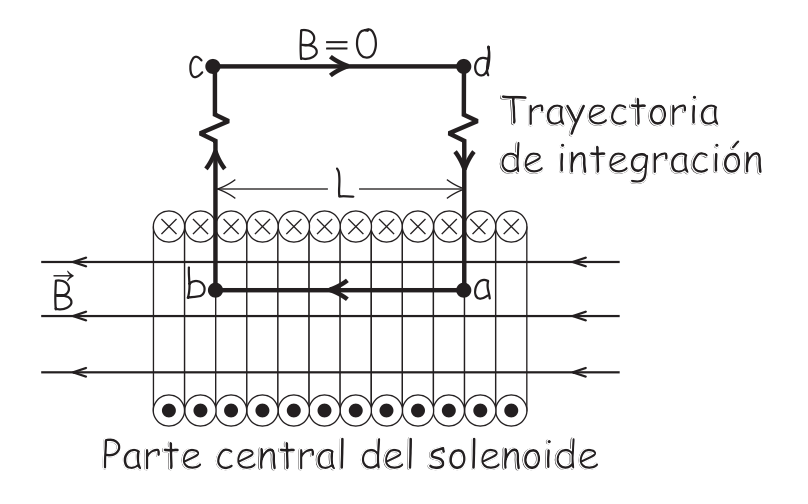
\includegraphics[scale=0.4]{fig/solenoide2}
\end{figure}
Aplicando la ley de Ampere, (\ref{28.20.ampere}), junto con la trayectoria mostrada, se tiene que 
\begin{equation}
B=\mu_0nI
\end{equation}
teniendo en cuenta que $I_{enc}=nLI$.
\subsection{Campo de un solenoide toroidal(toroide)}
\begin{figure}[t]
\centering
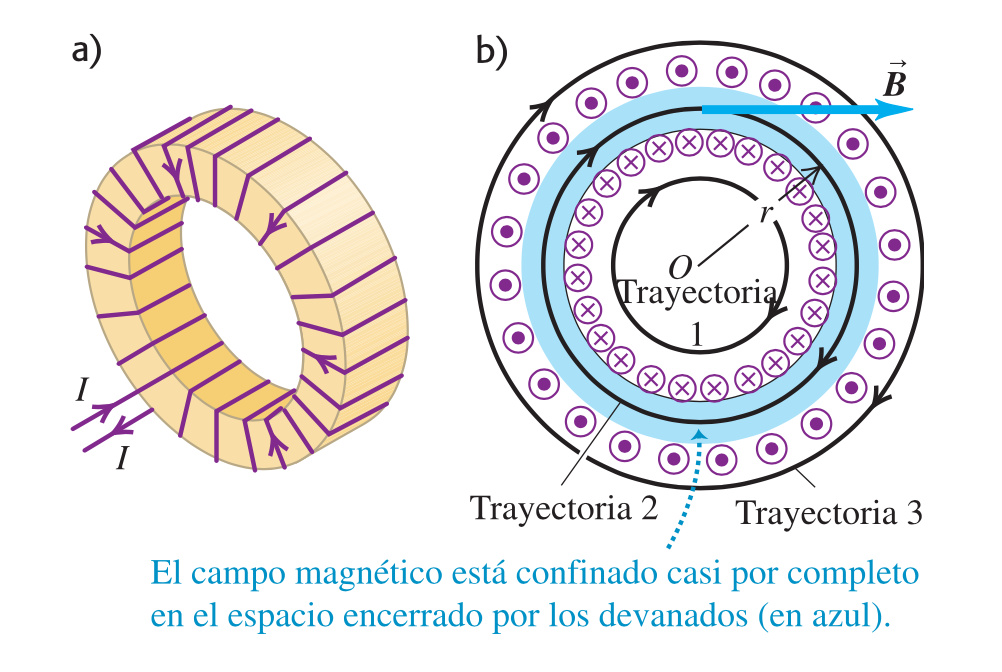
\includegraphics[scale=0.5]{fig/toroide}
\end{figure}
Considerando la trayectoria de integración 1. No hay corriente encerrada, luego $\vec{B}=0$ en cualquier punto de esta trayectoria.

Considernado la trayectoria de integración 3. Cada espira pasa dos veces a través del área limitada por esta trayectoria, llevando corrientes iguales en sentidos opuestos. Luego $I_{enc}=0\rightarrow \vec{B}=0$ en todos los puntos de esta trayectoria.

Considerando la trayectoria 2, un círculo con radio $r$. Se espera que el campo $\vec{B}$ sea tangente a la trayectoria. Por tanto, $\oint\vec{B}\cdot d\vec{l}=2\pi rB$. Despejando $B$
\begin{equation}\label{28.24.toroide}
B=\frac{\mu_0NI}{2\pi r}
\end{equation}
%\end{document}

\chapter{Inducción electromagnética}
La fuente de fem no es una batería, sino una estación generadora de electricidad.
La inducción electromagnética nos dice que un campo magnético que varía en el tiempo actúa como fuente de campo eléctrico.
También, un campo eléctrico que varía con el tiempo actúa como fuente de un campo magnético

\section{Ley de Faraday}
El flujo magnético total $\Phi_B$ a través de un área finita es la integral de esta expresión sobre el área:
\begin{equation}\label{29.1}
\Phi_B=\int\vec{B}\cdot d\vec{A}=\int B\, dA\cos\phi
\end{equation}
En el caso de que $\vec{B}$ sea uniforme sobre un área plana $\vec{A}$, entonces
\begin{equation}\label{29.2}
\Phi_B=\vec{B}\cdot \vec{A}=BA\cos\phi
\end{equation}
La \textbf{Ley de Faraday de la inducción} establece lo siguiente:
\textit{La fem inducida en una espira cerrada es igual al negativo de la tasa de cambio del flujo magnético a través de la espira con respecto al tiempo}.
 
En símbolos
\begin{equation}\marginnote{Ley de Faraday}\label{29.3.faraday}
\boxed{\varepsilon=-\frac{d\Phi_B}{dt}}
\end{equation}
\textbf{Obervación}: Las fem inducidas son ocasionadas por \textbf{cambios de flujo}.

Si se tiene una bobina con $N$ espiras idénticas y si el flujo varía a la misma tasa a través de cada espira, la fem total en la bobina es
\begin{equation}\label{29.4.Nfaraday}
\boxed{\varepsilon=-N\frac{d\Phi_B}{dt}}
\end{equation}
La \textbf{Ley de Lenz} establece que, \textit{la dirección de cualquier efecto de la inducción magnética es la que se opone a la causa del efecto.}
\section{Fuerza electromotriz de movimiento}
\begin{figure}[h]
\centering
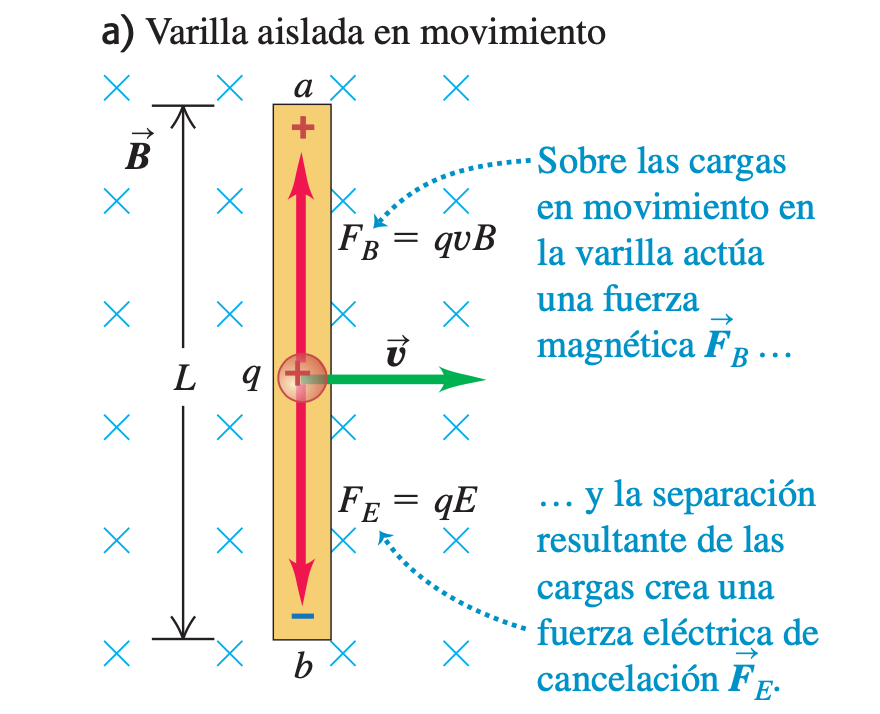
\includegraphics[scale=0.5]{fig/varilla}
\end{figure}
Una partícula cargada $q$ (	que suponemos positiva) en la varilla experimenta una fuerza magnética $\vec{F}=q\vec{v}\times\vec{B}$ con magnitud $F=|q|vB$. Esta fuerza magnética hace que las cargas libres en la varilla se muevan, lo que crea un exceso de carga positiva en el extremo superior $a$ y de carga negativa en el extremo inferior $b$.
Esto, a la vez, crea un campo eléctrico $\vec{E}$ en el interior de la varilla, en el sentido que va de $a$ hacia $b$ (opuesto al campo magnético). Llega un momento en el que $\vec{E}$ es lo suficientemente grande como para que la fuerza eléctrica ($qE$) cancele exáctamente a la magnética. De esta manera, $qE=qvB$, y las cargas están en equilibrio. Luego, se tiene que
\begin{equation}\label{29.5}
V_{ab}=V_a-V_b=EL=qBL
\end{equation}
con el punto $a$ a un potencial mayor que $b$.
\textbf{Continua...}
\subsection{Fem de movimiento: Forma general}
Podemos generalizar el concepto de fem de movimiento para un conductor de cualquier forma que se mueva en un campo magnético, uniforme o no (suponiendo que el campo magnético en cada punto no varía con el tiempo). Para cualquier fem cerrada, la fem total es
\begin{equation}\label{29.7}
\varepsilon=\oint (\vec{v}\times\vec{B})\cdot d\vec{l}
\end{equation}
Cuando se tienen conductores fijos en campos magnéticos cambiantes, no es posible utilizar (\ref{29.7}). En tal caso utilizar la ley de Faraday (\ref{29.3.faraday}).


\section{Campo eléctricos inducidos}
Una fem inducida también se presenta cuando hay un flujo cambiante a través de un conductor fijo.

\begin{figure}[h]\label{fig:galvanometro}
\centering
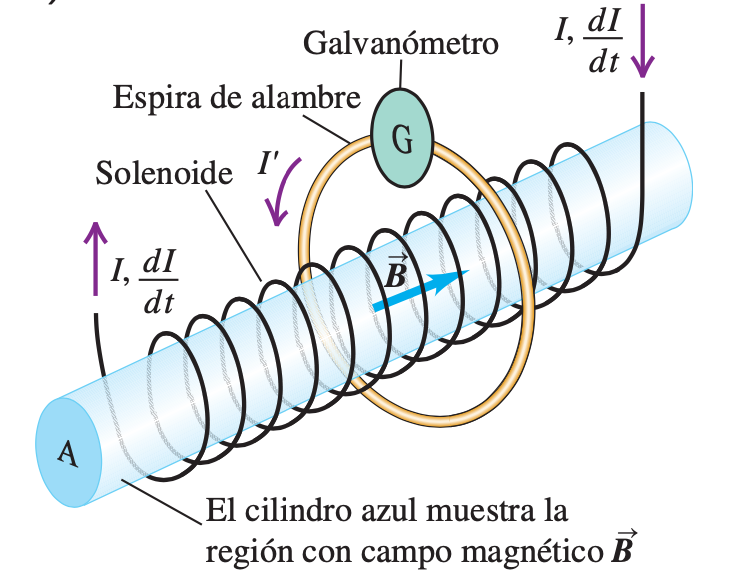
\includegraphics[scale=0.5]{fig/galvanometro}
\caption{El devanado de un solenoide largo lleva una corriente que se incrementa a una tasa $dI>dt$. El flujo magnético en el solenoide aumenta a una tasa $d\Phi_B/dt$, y este flujo cambiante pasa a través de una espira de alambre. En la espira se induce una fem $\varepsilon= -d\Phi_B/dt$, la cual induce una corriente $I'$ que se mide con el galvanómetro G}
\end{figure}

Consideremos la situacion que se ilustra en la figura \ref{fig:galvanometro}. Un solenoide largo y delgado, con área de sección transversal $A$ y $n$ espiras por unidad de
longitud, está rodeado en su centro por una espira conductora circular. El galvanómetro G mide la corriente en la espira. Una corriente $I$ en el devanado del solenoide establece un campo magnético $\vec{B}$ a lo largo de su eje, como se indica, con magnitud $B=\mu_0nI$, donde $n$ es el número de espiras por unidad de longitud. El flujo magnético a traves de la espira es $$\Phi_B=BA=\mu_0nIA$$ Cuando la corriente $I$ cambia con el tiempo se tiene, según la ley de Faraday

\begin{equation}\label{29.8}
\varepsilon=-\frac{d\Phi_B}{dt}=-\mu_0nA\frac{dI}{dt}
\end{equation}

Si la resistencia total de la espira es $R$, la corriente inducida en la espira es $I'=\varepsilon/R$. ¿Qué fuerza hace que las cargas se muevan alrededor de la espira? No puede ser una fuerza magnética porque el conductor no se está moviendo en un campo magnético, y en realidad ni siquiera está en un campo magnético. Se debe a un \textbf{campo magnético inducido} en el conductor \textit{causado por el flujo magnético cambiante}. Este campo eléctrico en la espira \textbf{no es conservativo}, porque la integral de línea de $\vec{E}$ a lo largo de la trayectoria cerrada no es igual a cero. En vez de ello, esta integral de línea, que representa el trabajo realizado por el campo inducido $\vec{E}$ por unidad de carga, es igual a la fem inducida $\varepsilon$:

\begin{equation}\label{29.9}
\oint\vec{E}\cdot d\vec{l}=\varepsilon
\end{equation}

Que según la ley de Faraday

\begin{equation}\label{29.10}\marginnote{Trayectoria de integración constante}
\boxed{\oint\vec{E}\cdot d\vec{l}=-\frac{d\Phi_B}{dt}}
\end{equation}

La forma de la ley de Faraday (\ref{29.10}), sólo es válida si la trayectoria alrededor de la cual se integra es \textbf{constante}.

Un campo de esta clase recibe el nombre de \textbf{campo no electrostático}. Este campo, a pesar de no ser conservativo, ejerce una fuerza $\vec{F}=q\vec{E}$ sobre una carga $q$. De esta manera, un campo magnético actúa como fuente de campo eléctrico de una clase que \textit{no podemos} producir con ninguna distribución de carga estática.

\section{Corriente de desplazamiento y ecuaciones de Maxwell}
De igual manera que un campo magnético que varía da lugar a un campo eléctrico inducido, un campo eléctrico variable, da lugar a un campo magnético.

\subsubsection{Generalización de la ley de Ampere}

\begin{figure}[h]
\centering
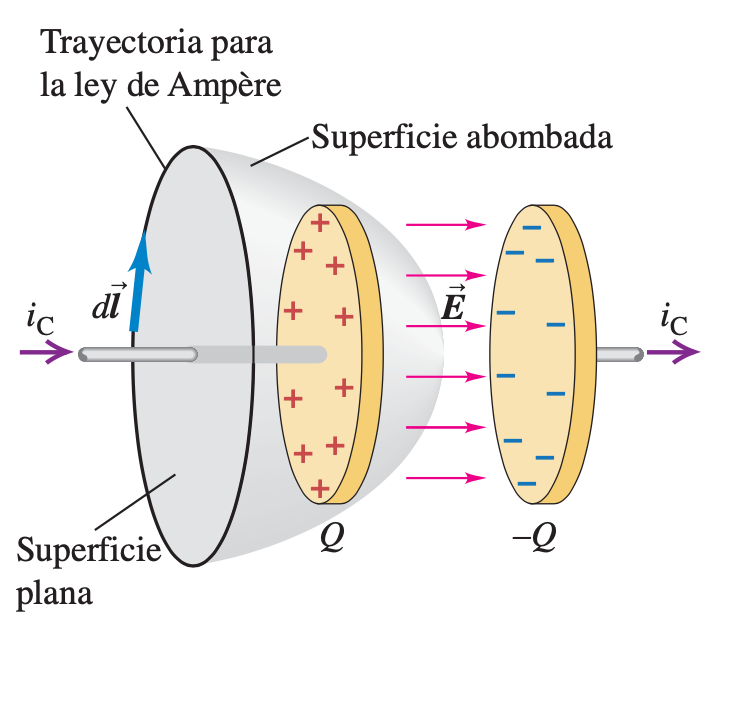
\includegraphics[scale=0.5]{fig/corriente-desplazamiento}
\caption{ Capacitor de placas paralelas en proceso de carga. La corriente de conducción a través de la superficie plana es $i_C$, pero no hay corriente de conducción a través de la superficie que se abomba para pasar entre las placas. Las dos superficies tienen una frontera común, por lo que esta diferencia en Ienc lleva a una contradicción aparente al aplicar la ley de Ampère.}
\label{fig:corriente-desplazamiento}
\end{figure}

Recordando la ley de Ampere, $$\oint\vec{B}\cdot d\vec{l}=\mu_0I_{enc}$$ Esta ley, expresada de esta manera está \textit{incompleta}. Consideremos la figura \ref{fig:corriente-desplazamiento}. Alambres conductores llevan corriente $i_C$\footnote{La notación $i_C$ indica corriente de conducción para diferenciarla de otra clase de corriente que vamos a encontrar y que se llama corriente de desplazamiento, $i_D$.} hacia una placa y fuera de la otra; la carga $Q$ se incrementa, y el campo eléctrico $\vec{E}$ entre las placas aumenta.

Apliquemos la ley de Ampère a la trayectoria circular que se muestra.  La integral $\oint\vec{B}\cdot\, d\vec{l}$ alrededor de esta trayectoria es igual a $\mu_0I_{enc}$. Para el área circular plana limitada por el círculo, $II_{enc}$ es tan sólo la corriente $i_C$ en el conductor de la izquierda. Pero la superficie que se abomba hacia la derecha está delimitada por el mismo círculo y la corriente a través de esa superficie es igual a cero. Por lo tanto, $\oint\vec{B}\cdot d\vec{l}$ es igual a $\mu_0I_{enc}$, y ¡al mismo tiempo es igual a cero! Ésta es una contradicción evidente.

Pero algo más ocurre en la superficie abombada. A medida que el capacitor se carga, el campo eléctrico $\vec{E}$ y el flujo eléctrico $\Phi_E$ a través de la superficie aumentan. La carga instantánea es $q=Cv$. Para un capacitor de placas paralelas, $C=\epsilon_0A/d$, donde $A$ es el área de las placas y $d$ es la separación. La diferencia de potencial $v$ entre las placas es $v=Ed$.

Al sustituir estas expresiones para $C$ y $v$ en $q = Cv$, la carga en el capacitor, $q$, se expresa como	

\begin{equation}\label{29.12}
q=Cv=\frac{\epsilon A}{d}(Ed)=\epsilon EA=\epsilon\Phi_E
\end{equation}


Derivando (\ref{29.12}) con respecto al tiempo se obtiene

\begin{equation}\label{29.13}
\boxed{i_C=\frac{dq}{dt}=\epsilon\frac{d\Phi_E}{dt}}
\end{equation}


Ahora, con un pequeño esfuerzo de imaginación, inventamos una \textbf{corriente de desplazamiento} ficticia, $i_D$, en la región entre las placas, definida como

\begin{equation}\label{29.14}\marginnote{Corriente de desplazamiento}
\boxed{i_D=\epsilon\frac{d\Phi_E}{dt}}
\end{equation}
 Es decir, imaginamos que el flujo cambiante a través de la superficie curva en la figura \ref{fig:corriente-desplazamiento} es en cierto modo equivalente, en la ley de Ampère, a una corriente de conducción a través de esa superficie. Incluyéndola en la ley de Ampère
 
\begin{equation}\label{29.15}\marginnote{Ley de Ampère generalizada}
\boxed{\oint\vec{B}\cdot d\vec{l}=\mu_0(i_C+i_D)_{enc}}
\end{equation}

La ley de Ampère planteada en esta forma es obedecida sin importar cuál superficie se use en la figura \ref{fig:corriente-desplazamiento}. Para la superficie plana, $i_D$ es igual a cero; para la superficie curva, $i_C$ es cero; e $i_C$ para la superficie plana es igual a $i_D$ para la superficie curva.

Hay una \textit{densidad de corriente de desplazamiento} correspondiente$j_D=i_D/A$; a partir de $\Phi_E=EA$ y dividiendo (\ref{29.14}) entre $A$, se encuentra

\begin{equation}\label{29.16}
j_D=\epsilon\frac{dE}{dt}
\end{equation}

\subsection{Ecuaciones de Maxwell del electromagnetismo}
Por ahora, enunciaremos las ecuaciones de Maxwell en su forma más sencilla, para el caso en que hay cargas y corrientes en un espacio en que, por lo demás, está vacío.

\begin{equation}\label{29.18.1}\marginnote{Ley de Gauss para $\vec{E}$}
\boxed{\oint\vec{E}\cdot  d\vec{A}=\frac{Q_{enc}}{\epsilon_0}}
\end{equation}

\begin{equation}\label{29.19.1}\marginnote{Ley de Gauss para $\vec{B}$}
\boxed{\oint\vec{B}\cdot  d\vec{A}=0}
\end{equation}

Este enunciado significa, entre otras cosas, que no hay monopolos magnéticos (cargas magnéticas individuales) que actúen como fuentes del campo magnético.

\begin{equation}\label{29.20.1}\marginnote{Ley de Ampère}
\boxed{\oint\vec{B}\cdot  d\vec{l}=\mu_0\left(i_C+\epsilon_0\frac{d\Phi_E}{dt}\right)}
\end{equation}

\begin{equation}\label{29.21.1}\marginnote{Ley de Faraday}
\boxed{\oint\vec{E}\cdot  d\vec{l}=-\frac{d\Phi_B}{dt}}
\end{equation}

Si hay un flujo magnético cambiante, la integral de línea en (\ref{29.21.1}) es diferente de cero, lo que demuestra que el campo $\vec{E}$ producido por un flujo magnético cambiante no es conservativo. Recuerde que esta integral de línea debe llevarse a cabo sobre una trayectoria cerrada \textit{constante}.

\subsection{Simetría en las ecuaciones de Maxwell}
Las ecuaciones (\ref{29.20.1}) y (\ref{29.21.1}) se pueden volver a escribir en forma distinta pero equivalente incluyendo las definiciones de flujo eléctrico y flujo magnético, $\Phi_E=\int	\vec{E}\cdot d\vec{A}$ y $\Phi_B=\int\vec{B}\cdot d\vec{A}$, respectivamente. En el espacio vacío, donde no hay carga ni corriente de conducción, $i_C = 0$ y $Q_{enc} = 0$, y tenemos

\begin{equation}\label{29.22}
\oint\vec{B}\cdot d\vec{l}=\epsilon_0\mu_0\frac{d}{dt}\int	\vec{E}\cdot d\vec{A}
\end{equation}

\begin{equation}\label{29.23}
\oint\vec{E}\cdot d\vec{l}=-\frac{d}{dt}\int	\vec{B}\cdot d\vec{A}
\end{equation}

La característica más notable de estas ecuaciones es que un campo de \textit{cualquier} tipo que varíe con respecto al tiempo induce un campo del otro tipo en las regiones vecinas del espacio.





























%\end{document}

\chapter{Inductancia}
\section{Inductancia mutua}

\begin{figure}[h]
\centering
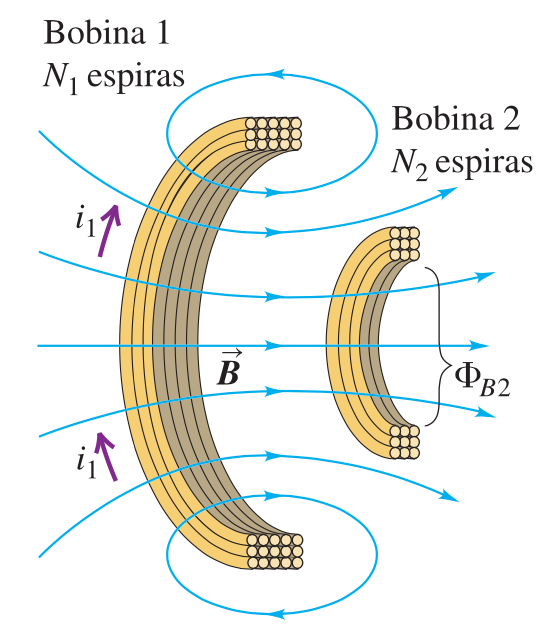
\includegraphics[scale=0.3]{fig/bobinas}
\caption{\textbf{Inductancia mutua}, si la corriente en la bobina 1 está cambiando, el flujo cambiante a través de la bobina 2 indice una fem en esta última}
\label{fig:bobinas}
\end{figure}
Interacción magnética entre dos alambres que trasnportan corrientes \textit{estables}; la corriente de uno de los alambres genera un campo magnético que ejerce una fuerza sobre la corriente entre el otro alambre. Cuando hay una corriente \textit{variable} en uno de los circuitos, surge una interacción adicional. Consideremos la situación de la figura
\ref{fig:bobinas}

Una corriente que circula por la bobina 1 produce un campo magnético $\vec{B}$ y, por lo tanto, un flujo magnético a través de la bobina 2. Si la corriente en la bobina 1 cambia, el flujo a través de la bobina 2 también cambia; de acuerdo con la ley de Faraday, esto induce una fem en la bobina 2. De este modo, un cambio en la corriente de un circuito puede inducir otra corriente en un segundo circuito.
Una corriente $i_1$\footnote{Denotamos con $i$ a una corriente variable en el tiempo } establece un campo magnético (indicado por las líneas de color azul), y algunas de estas líneas de campo pasan a través de la bobina 2. Denotaremos con $\Phi_{B2}$ el flujo magnético a través de \textit{cada} espira de la bobina 2, causado por la corriente $i_1$ en la bobina 1. (Si el flujo es diferente a través de las distintas espiras de la bobina, entonces $\Phi_{B2}$ denota el flujo  \textit{medio}). El campo magnético es proporcional a $i_1$, de manera que $\Phi_{B2}$ también es proporcional a $i_1$. \textbf{Cuando $i_1$ cambia, $\Phi_{B2}$ cambia; este flujo cambiante induce una fem $\varepsilon_2$ en la bobina 2}, dada por
\begin{equation}\label{fem}
\varepsilon_2=-N_2\frac{d\Phi_{B2}}{dt}
\end{equation}
Podríamos representar la proporcionalidad entre $\Phi_{B2}$ e $i_1$ en la forma $\Phi_{B2}$ = (constante) $i_1$, pero, en vez de ello, es más conveniente incluir el número de espiras $N_2$ en la relación. Al introducir una constante de proporcionalidad $M_{21}$, llamada \textbf{inductancia mutua} de las dos bobinas, escribimos
\begin{equation}\label{30.2}
N_2\Phi_{B2}=M_{21}i_1
\end{equation}
donde $\Phi_{B2}$ es el flujo a través de una sola espira de la bobina 2. De ahí que,
\begin{equation}
N_2\frac{d\Phi_{B2}}{dt}=M_{21}\frac{di_1}{dt}
\end{equation}
y (\ref{fem}) se rescribe como
\begin{equation}
\varepsilon_2=-M_2\frac{di_1}{dt}
\end{equation}
Es decir, un cambio en la corriente $i_1$ en la bobina 1 induce una fem en la bobina 2, que es directamente proporcional a la tasa de cambio de $i_1$.

También se podría escribir la definición de la inductancia mutua, (\ref{30.2}), como
\begin{equation}
M_{21}=\frac{N_2\Phi_{B2}}{i_1}
\end{equation}
\textbf{Si las bobinas están en el vacío}, el flujo $\Phi_{B2}$ a través de cada espira de la bobina 2 es directamente proporcional a la corriente $i_1$. Entonces, la inductancia mutua $M_{21}$ es una constante que sólo depende de la geometría de las dos bobinas.
Podría volverse a hacer el análisis para el caso opuesto, en el que una corriente cambiante $i_2$ en la bobina 2 causa un flujo cambiante $\Phi_{B}2$ y una fem $\varepsilon_1$ en la bobina 1. Se encuentra que, \textbf{$M_{12}$ siempre es igual a $M_{21}$, aun cuando las dos bobinas no sean simétricas}. A este valor común $M$ lo llamamos simplemente \textbf{inductancia mutua}. Por tanto, tenemos:
\begin{equation}\marginnote{Fem mutuamente inducidas}
\boxed{\varepsilon_2=-M\frac{di_1}{dt}\quad\mathrm{y}\quad \varepsilon_1=-M\frac{di_2}{dt}\quad}
\end{equation}
donde la inductancia mutua $M$ es
\begin{equation}\marginnote{Inductancia mutua}
\boxed{M=\frac{N_2\Phi_{B2}}{i_1}=\frac{N_1\Phi_{B1}}{i_2}}
\end{equation}
\textbf{Obs: Sólo una corriente variable en el tiempo induce una fem}.

La unidad del SI para la inductancia mutua se llama \textbf{henry} [$H$]
\section{Autoinductancia a inductores}
\begin{figure}[h]
\centering
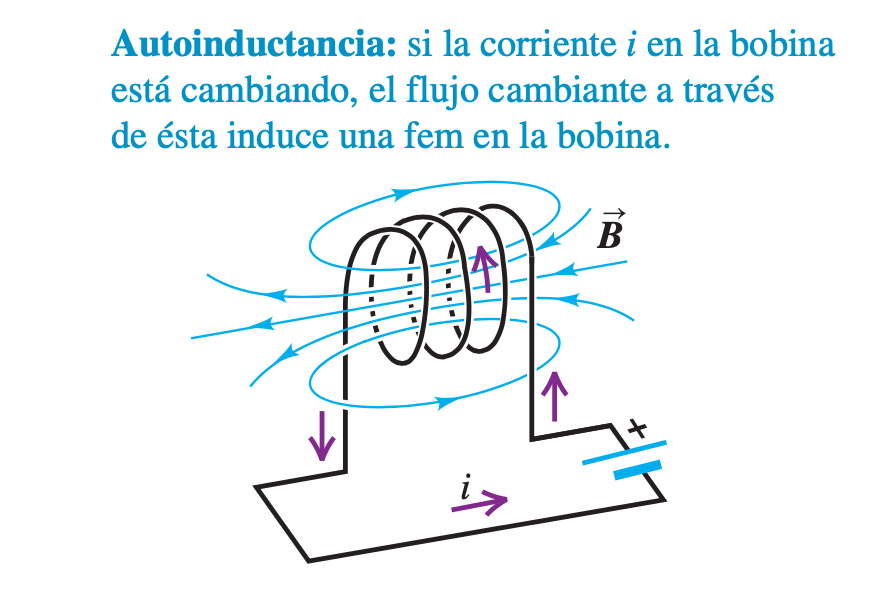
\includegraphics[scale=0.4]{fig/autoinductancia}
\caption{La corriente $i$ en el circuito crea un campo magnético $\vec{B}$ en la bobina y, por lo tanto, un flujo a través de ésta.}
\label{fig:autoinductancia}
\end{figure}

Consideremos un solo circuito aislado. Cuando en el circuito está presente una corriente, se establece un campo magnético que crea un flujo magnético a través del mismo circuito; este flujo cambia cuando la corriente cambia. Así, cualquier circuito que conduzca una corriente variable tiene una fem inducida en él por la variación en su propio campo magnético. Esa clase de fem se denomina \textbf{fem autoinducida}. Según la ley de Lenz, una fem autoinducida siempre se opone al cambio en la corriente que causó la fem, y de ese modo hace más difícil que haya variaciones en la corriente. El efecto se intensifica considerablemente si el circuito incluye una bobina con $N$ espiras de alambre. Como resultado de la corriente $i$, hay un flujo magnético medio $\Phi_B$ a través de cada vuelta de la bobina, figura \ref{fig:autoinductancia}.

Definimos la \textbf{autoinductancia} como
\begin{equation}\label{30.6.autoinductancia}\marginnote{Autoinductancia}
\boxed{L=\frac{N\Phi_B}{i}}
\end{equation}
Si la corriente $i$ en el circuito cambia, también lo hace el flujo $\Phi_B$. De ecuación \ref{30.6.autoinductancia} $$N\frac{d\Phi_B}{dt}=L\frac{di}{dt}$$ Utilizando la ley de Faraday, (\ref{29.4.Nfaraday}), la fem autoinducida es
\begin{equation}\label{30.7}\marginnote{Fem autoinducida}
\boxed{\varepsilon=-L\frac{di}{dt}}
\end{equation}

\subsection{Los inductores como elementos de un circuito}
Un elemento de circuito diseñado para tener una inductancia particular se llama \textbf{inductor, o bobina de autoinducción}. Su finalidad es oponerse a cualquier variación en la corriente a través del circuito. Un inductor en un circuito de corriente directa ayuda a mantener una corriente estable a pesar de las fluctuaciones en la fem aplicada; en un circuito de corriente alterna, un inductor tiende a suprimir las variaciones de la corriente que ocurran más rápido de lo deseado.

Al utilizar la ley de Kirchhoff a traves de una malla conductora se suman sus diferencias de potencial y se igualan a cero porque el campo eléctrico producido por las cargas distribuidas es \textit{conservativo} ($\vec{E_c}$). El campo eléctrico inducido magnéticamente dentro de las bobinas del inductor \textbf{no es conservativo} ($\vec{E_n}$).


\begin{figure}[h]
\centering
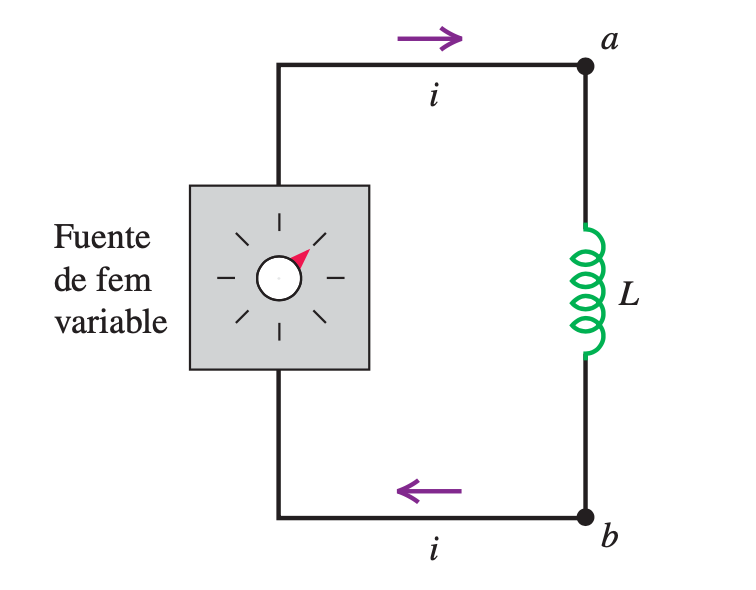
\includegraphics[scale=0.4]{fig/circuito}
\caption{Circuito que contiene una fuente de fem y un inductor. La fuente es variable, por lo que la corriente $i$ y su tasa de cambio $di>dt$ pueden variarse.}
\label{fig30.5.circuito}
\end{figure}

Consideremos el circuito de la figura \ref{fig30.5.circuito}. De acuerdo con la ley de Faraday, (\ref{29.10}), la integral de línea de $\vec{E_n}$ alrededor del circuito es el negativo de la tasa de cambio del flujo a través del circuito. De (\ref{30.7}) $$\oint\vec{E_n}\cdot d\vec{l}=-L\frac{di}{dt}$$ donde se integra en sentido horario del circuito (el sentido supuesto para la corriente). Pero $\vec{E_n}$ es diferente de cero sólo dentro del inductor. Entonces $$\int_a^b\vec{E_n}\cdot d\vec{l}=-L\frac{di}{dt}$$ A continuación, como $\vec{E_c}+\vec{E_n}=0$ en cada punto dentro de las bobinas del inductor $$\int_a^b\vec{E_c}\cdot d\vec{l}=L\frac{di}{dt}$$ Pero esta integral es el potencial $V_{ab}$ del punto $a$ con respecto a $b$

\begin{equation}\label{30.8}
V_{ab}=V_a-V_b=L\frac{di}{dt}
\end{equation}

Se concluye que hay una diferencia de potencial genuina entre las terminales del inductor, asociada con las fuerzas conservativas electrostáticas, a pesar del hecho de que el campo eléctrico asociado con el efecto de inducción magnética es no conservativo.
\textbf{Obervación}: La fem autoinducida se opone a los cambios de la corriente ($di/dt$), \textit{no} a la corriente $i$ en sí.

\section{Energía del campo magnético}
El establecimiento de una corriente en un inductor requiere un suministro de energía, y un inductor que conduce corriente contiene energía almacenada. En la figura \ref{fig30.5.circuito}, una \textit{corriente creciente} $i$ ($di/dt>0$) en el inductor produce una fem $\varepsilon$ entre sus terminales, y una diferencia de potencial correspondiente $V_{ab}$ entre las terminales de la fuente, con el punto $a$ a mayor potencial que el $b$. Así, la fuente debe estar agregando energía al inductor, y la potencia instantánea $P$ (la tasa de transferencia de energía al inductor) es $P=V_{ab}i$.

\subsection{Energía almacenada en un inductor}
Si la corriente inicial es igual a cero, con la inductancia $L$ podemos calcular la entrada total de energía $U$ necesaria para establecer una corriente final $I$ en un inductor. Suponemos que el inductor tiene una resistencia igual a cero, por lo que dentro del inductor no se disipa energía. El voltaje entre las terminales $a$ y $b$ del inductor en ese instante es $V_{ab}=L\frac{di}{dt}$, y la tasa $P$ a la que se entrega energía al indutor (igual a la potencia instantánea suministrada por la fuente) es

\begin{equation*}
P=V_{ab}i=Li\frac{di}{dt}
\end{equation*}

La energía $dU$ suministrada al inductor durante un intervalo de tiempo infinitesimal $dt$ es $dU=Pdt$, por lo que

\begin{equation*}
dU=Lidi
\end{equation*}

La energía total $U$ suministrada mientras la corriente aumenta de cero a un valor final
$I$ es

\begin{equation}\label{30.9}\marginnote{Energía almacenada en un inductor}
\boxed{U=L\int_0^{I}i\, dt=\frac{1}{2}LI^2}
\end{equation}

Una vez que la corriente ha alcanzado su valor final estable $I$, $di/dt=0$, y no se alimenta más energía al inductor. Cuando no hay corriente, la energía almacenada $U$ es igual a cero; cuando la corriente es $I$, la energía es $\frac{1}{2}LI^2$.

Cuando la corriente disminuye de $I$ a cero, el inductor actúa como fuente que suministra una cantidad total de energía igual a $\frac{1}{2}LI^2$ al circuito externo. Si interrumpimos bruscamente el circuito abriendo un interruptor o desconectando violentamente una clavija (enchufe) de una toma de corriente de pared, la corriente disminuye con mucha rapidez, la fem inducida es muy grande y la energía podría disiparse en forma de un arco entre los contactos del interruptor.

\textbf{Observación:} Es importante no confundir el comportamiento de resistores e inductores en lo que respecta a la energía. La energía fluye hacia un resistor siempre que una corriente, ya sea estable o variable, pasa a través de él; esta energía se disipa en forma de calor. En contraste, la energía fluye hacia un inductor ideal con resistencia igual a cero, sólo cuando la corriente en este último se \textit{incrementa}. Esta energía no se disipa, sino que se almacena en el inductor y se libera cuando la corriente \textit{disminuye}. Cuando una corriente estable fluye a través de un inductor, no entra ni sale energía

\subsection{Densidad de la energía magnética}
La energía en un inductor en realidad se almacena en el campo magnético dentro de la bobina, al igual que la energía de un capacitor lo hace en el campo eléctrico entre sus placas. Nos centraremos en un caso sencillo: el del solenoide toroidal ideal. Su campo magnético se encuentra confinado por completo en una región finita del espacio en el interior de su núcleo. La inductancia del selenoide toroidal con vacío dentro de sus bobinas es 

\begin{equation}\label{L de un toroide}\marginnote{Inductancia de un toroide}
L=\frac{\mu_0N^2A}{2\pi r}
\end{equation}

De (\ref{30.9}), la energía $U$ alamacenada en el toroide  cuando la corriente es $I$ es

\begin{equation*}
U=\frac{1}{2}LI^2=\frac{1}{2}\frac{\mu_0N^2A}{2\pi r}I^2
\end{equation*}

El campo magnético y, por lo tanto, esta energía se localizan en el volumen $V=2\pi rA$ encerrado por los devanados. La energía por \textit{unidad de volumen}, o \textit{densidad de energía magnética}, es $u=U/V$:

\begin{equation}\label{u}
u=\frac{U}{2\pi rA}=\frac{1}{2}\mu_0\frac{N^2I^2}{(2\pi r)^2}
\end{equation}

Expresandola en términos de la magnitud $B=(\mu_0NI)/(2\pi r)$ del campo magnético dentro del toroide es

\begin{equation*}
\frac{N^2I^2}{(2\pi r)^2}=\frac{B^2}{\mu_0^2}
\end{equation*}

Sustituyendo esto en (\ref{u}), se encuentra que la expresión para la \textbf{densidad de energía magnética} en el vacío es

\begin{equation}\label{30.10.u}\marginnote{Densidad de energía magnética en el vacío}
\boxed{u=\frac{B^2}{2\mu_0}}
\end{equation}

Cuando el material dentro del toroide no es un vacío, sino un material con permeabilidad magnética (constante) $\mu=K_m\mu_0$, se sustituye $\mu_0$ por $\mu_0$ en (\ref{30.10.u}). Así, la energía por unidad de volúmen en el campo magnético es

\begin{equation}\label{30.11.u2}\marginnote{Densidad de energía magnética en un material}
\boxed{u=\frac{B^2}{2\mu}}
\end{equation}

La expresión \ref{30.11.u2} resulta ser correcta para \textit{cualquier} configuración de campo magnético en un material con permeabilidad constante. 

\section{El circuito R-L}
Un inductor en un circuito hace difícil que ocurran cambios rápidos en la corriente, en virtud de los efectos de la fem autoinducida. La ecuación \ref{30.7} muestra que cuanto más grande es la tasa de cambio de la corriente, $di/dt$, mayor es la fem autoinducida y mayor la diferencia de potencial entre las terminales del inductor.

\subsection{Crecimiento de la corriente en un circuito R-L}

\begin{figure}[h]
\centering
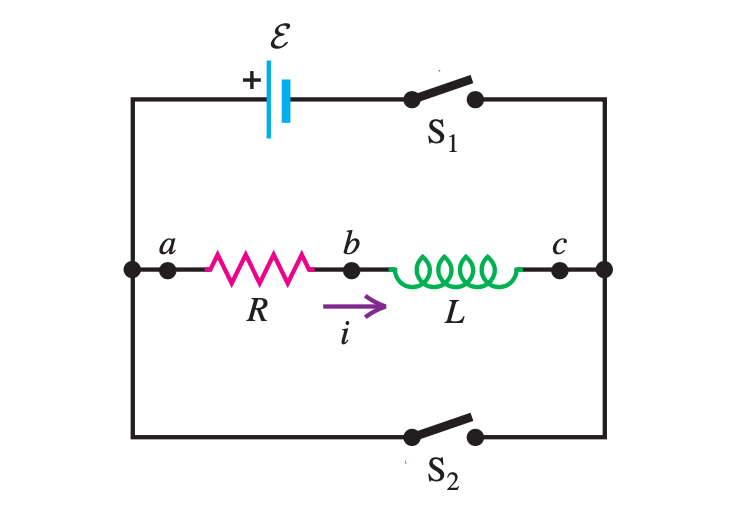
\includegraphics[scale=0.4]{fig/circuito2}
\caption{Al cerrar el interruptor $S_1$ se conecta la combinación $R-L $en serie con una fuente de fem $\varepsilon$. Al cerrar el interruptor $S_2$ al mismo tiempo que se abre $S_1$ se desconecta la combinación de la fuente.}
\label{fig:circuito2}
\end{figure}

Un circuito que incluye tanto un resistor como un inductor, y tal vez una fuente de fem, se llama circuito R-L (figura \ref{fig:circuito2}).  El inductor ayuda a impedir los cambios rápidos en una corriente, lo que puede ser útil si se requiere una corriente estable y la fuente externa tiene una fem fluctuante. Al cerrar el interruptor $S_1$ se conecta la combinación R-L a una fuente con fem constante $\varepsilon$. 

Suponga que, en un principio, ambos interruptores están abiertos, y luego, en cierto momento inicial $t=0$ se cierra el interruptor $S_1$. La corriente no puede cambiar súbitamente de cero a algún valor final porque $di/dt$ y la fem inducida en el inductor serían infinitas. En vez de ello, la corriente comienza a crecer con una tasa que sólo depende del valor de $L$ en el circuito.

Sea $i$ la corriente en cierto momento $t$ después de que se cerró el interruptor $S_1$, y sea $di/dt$ su tasa de cambio en ese instante. La diferencia de potencial $v_{ab}$ a través del resistor en ese momento es

\begin{equation*}
v_{ab}=iR
\end{equation*}

y la diferencia de potencial $v_{bc}$ a través del inductor es

\begin{equation*}
v_{bc}=L\frac{di}{dt}
\end{equation*}

Aplicamos la ley de mallas de Kirchhoff, comenzando en la terminal negativa y avanzando en sentido antihorario alrededor del circuito:

\begin{equation}\label{30.12}
\varepsilon - iR - L\frac{di}{dt}=0
\end{equation}
\begin{equation}\label{30.13}
\frac{di}{dt}=\frac{\varepsilon -iR}{L}=\frac{\varepsilon}{L}-\frac{R}{L}i
\end{equation}
 En el instante en que el interruptor $S_1$ se cierra por primera vez, $i = 0$ y la caída del potencial a través de $R$ es igual a cero. La tasa de cambio inicial de la corriente es
 
\begin{equation*}
\left(\frac{di}{dt}\right)_{inicial}=\frac{\varepsilon}{L}
\end{equation*}
 Como se esperaba, cuanto mayor es la inductancia $L$, con más lentitud aumenta la corriente.
 
Conforme aumenta la corriente, el término $(R/L)i$ en (\ref{30.13}) también aumenta, y la tasa de incremento de la corriente dada por (\ref{30.13}) se hace cada vez más pequeña. Esto significa que la corriente se acerca a un valor final $I$ de estado estable. Cuando la corriente alcanza ese valor, su tasa de incremento es igual a cero. Entonces, la ecuación \ref{30.13} se convierte en:

\begin{align*}
\left(\frac{di}{dt}\right)_{final}&=0=\frac{\varepsilon}{L}-\frac{R}{L}i \\
\Rightarrow  I&=\frac{\varepsilon}{R}
\end{align*}

La corriente \textit{final} $I$ no depende de la inductancia $L$; es la misma que se tendría si sólo se conectara la resistencia $R$ a la fuente con fem $\varepsilon$.

Para obtener el comportamiento de la corriente en función del tiempo, se reordena (\ref{30.13}):

\begin{equation*}
\frac{di}{i-(\varepsilon /R)}=-\frac{R}{L}dt
\end{equation*}

Cambiando el nombre de las variables de integración a $i'$ y $t'$ para utilizar $i$ y $t$ como límites superiores

\begin{align*}
\int_0^{i}\frac{di'}{i'-(\varepsilon /R)}&=-\int_0^{t}\frac{R}{L}dt' \\
\ln\left(\frac{i-(\varepsilon /R)}{-\varepsilon /R}\right)&=-\frac{R}{L}t
\end{align*}

Despejando la corriente $i$

\begin{equation}\label{30.14}\marginnote{Corriente en un circuito R-L con fem}
\boxed{i=\frac{\varepsilon}{R}(1-e^{-(R/L)t})}
\end{equation}

(\ref{30.14}) se obtiene

\begin{equation}\label{30.15}
\frac{di}{dt}=\frac{\varepsilon}{L}e^{-(R/L)t}
\end{equation}

En el momento $t=0$, $i=0$ y $di/dt=\varepsilon /L$. Conforme $t\to\infty$, $i\to \varepsilon /R$ y $di/dt\to 0$, como se había pronosticado. Este comportamiento se ve representado en la figura \ref{fig:rl-grafico}

\begin{figure}[h]
\centering
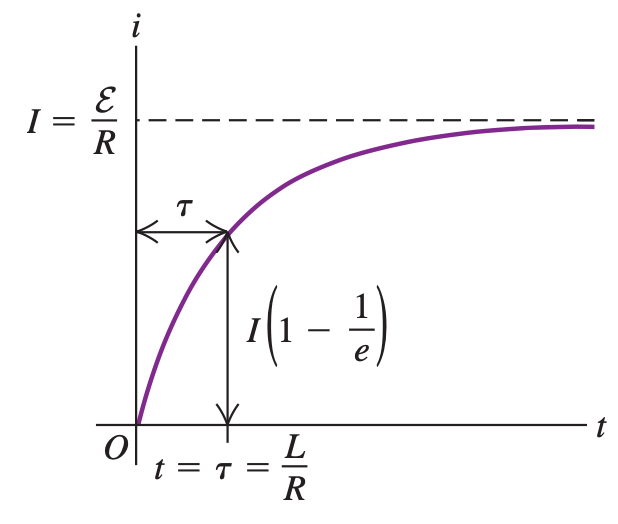
\includegraphics[scale=0.5]{fig/rl-grafico}
\caption{Curva de la ecuación \ref{30.14}}
\label{fig:rl-grafico}
\end{figure}

En un tiempo igual a $L/R$ la corriente ha subido a $(1-1/e)$, o el $63\%$ de su valor final. De esta forma, la cantidad $L/R$ es una medida de la rapidez con que la corriente se aproxima a su valor final; esta cantidad se llama \textit{constante de tiempo} del circuito, y se denota con $\tau$:

\begin{equation}\label{30.16}\marginnote{Constante de tiempo para un circuito R-L}
\tau=\frac{L}{R}
\end{equation}

Las consideraciones acerca de la energía brindan una perspectiva adicional sobre el comportamiento de un circuito R-L. La tasa instantánea con la que la fuente entrega energía al circuito es $P=\varepsilon i$. La tasa instantánea con que se disipa energía en el resistor es $i^2R$, y la tasa con que se almacena energía en el inductor es $iv_{bc}=Li\, di/dt$ [o, en forma equivalente, $(d/dt)(\frac{1}{2}Li^2)=Li\, di/dt$]. Multiplicando (\ref{30.12}) y reordenando se obtiene

\begin{equation}\label{30.17}
\varepsilon i=i^2R+Li\frac{di}{dt}
\end{equation}

De la potencia $\varepsilon i$ suministrada por la fuente, la parte $(i^2R)$ se disipa en el resistor, y la parte $(Li\, di/dt)$ es la energía almacenada en el inductor.

\subsection{Decaimiento de la corriente en un circuito R-L}
Ahora supongamos que el interruptor $S_1$ en el circuito de la figura \ref{fig:circuito2} ha permanecido cerrado por un tiempo y la corriente ha alcanzado el valor $I_0$. Se reinicia el cronómetro para redefinir el tiempo inicial, se cierra el interruptor $S_2$ en el momento $t=0$, con la batería puesta en derivación. La ecuación de la ley de Kirchhoff de las mallas se obtiene (\ref{30.12}), con sólo omitir el término $\varepsilon$. Haciendo los cálculos se ecuentra que la corriente varía con el tiempo de acuerdo con

\begin{equation}\label{30.18}
\boxed{i=I_0e^{-(R/L)t}}
\end{equation}

donde $I_0$ es la corriente inicial en el momento $t=0$

\begin{figure}[h]
\centering
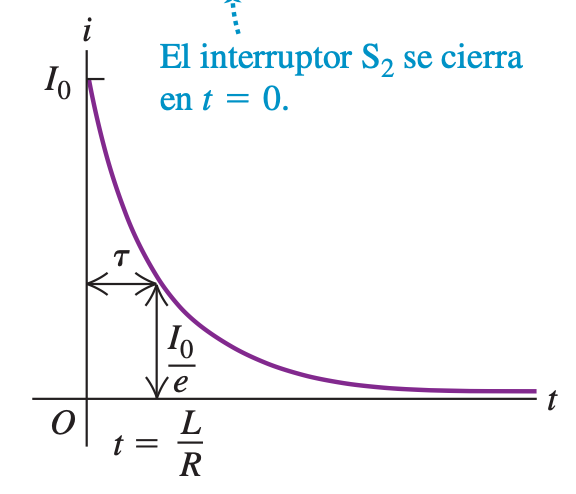
\includegraphics[scale=0.4]{fig/r-l-desconexion}
\caption{Curva de la ecuación \ref{30.18}}
\label{fig:r-l-desconexion}
\end{figure}

La energía necesaria para mantener la corriente durante este decaimiento proviene de la energía almacenada en el campo magnético del inductor. En vez de (\ref{30.17}) tenemos

\begin{equation}\label{30.19}
0=i^2R+Li\, \frac{di}{dt}
\end{equation}

\section{El circuito L-C}
Un circuito que contiene un inductor y un capacitor muestra un modo completamente nuevo de comportamiento, caracterizado por una corriente y una carga \textit{oscilantes}.

\begin{figure}[h]
\centering
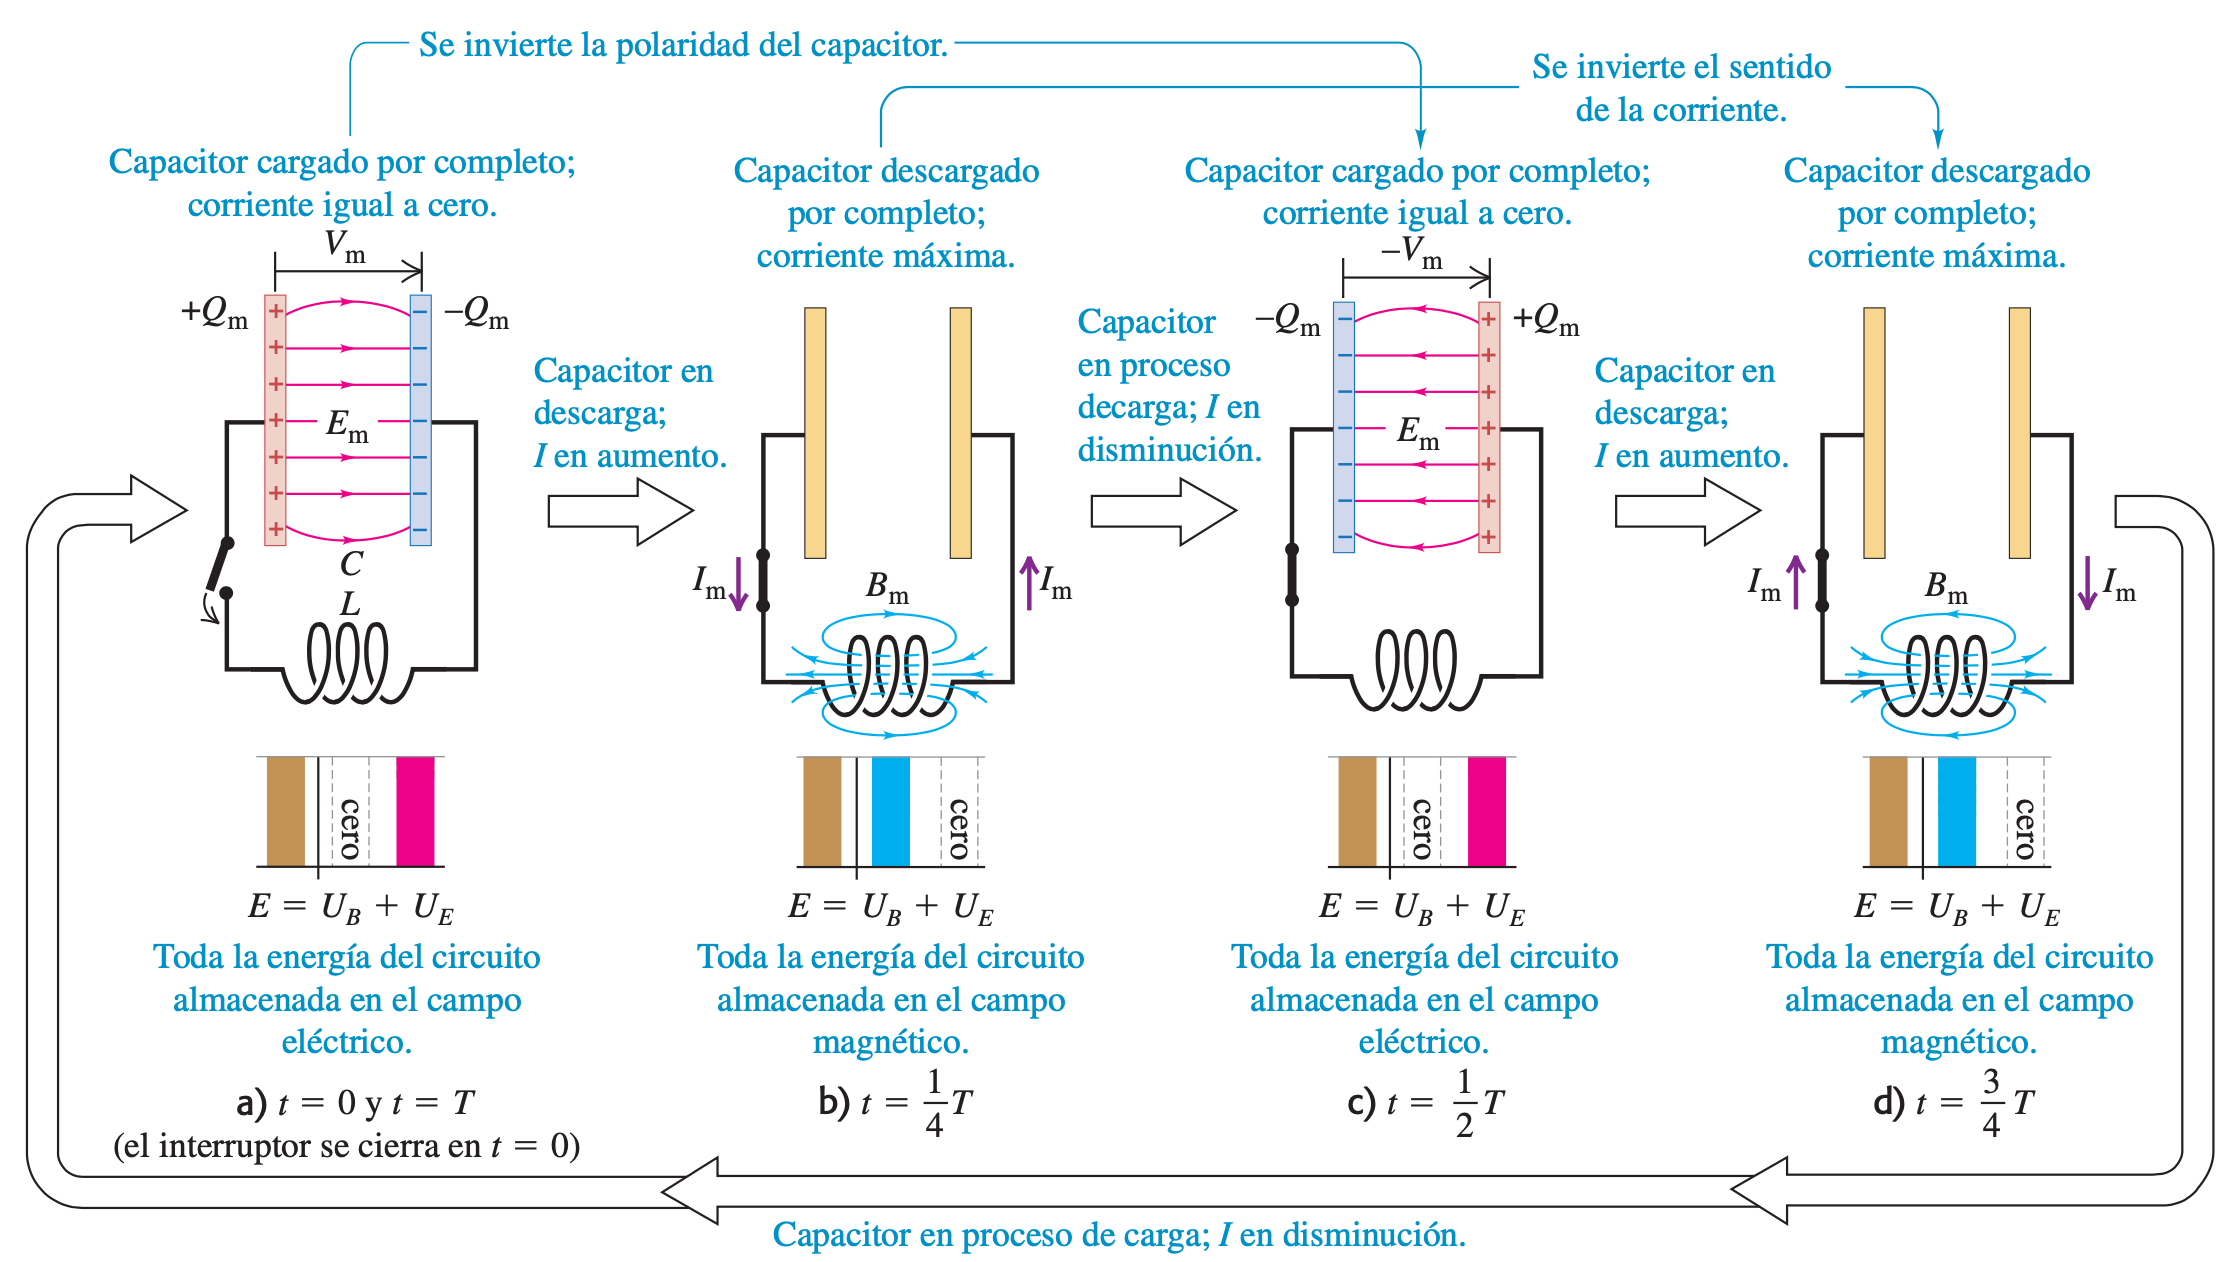
\includegraphics[scale=0.4]{fig/circuito-l-c}
\caption{En un circuito oscilante L-C, la carga en el capacitor y la corriente a través del inductor varían en forma sinusoidal con el tiempo. Se transfiere energía entre la energía magnética en el inductor $(U_B)$ y la energía eléctrica en el capacitor $(U_E)$. Como en el movimiento armónico simple, la energía total $E$ permanece constante.}
\label{fig:circuito-l-c}
\end{figure}

En el \textbf{circuito L-C} de la figura \ref{fig:circuito-l-c} se carga el capacitor con una diferencia de potencial $V_m$ y una carga inicial $Q=CV_m$ en su placa izquierda y luego se cierra el interruptor. El capacitor comienza a descargar a través del inductor. A causa de la fem inducida en el inductor, la corriente no puede cambiar en forma instantánea; comienza en cero y finalmente alcanza un valor máximo $I_m$. Durante esta intensificación el capacitor se está descargando. En cada instante el potencial del capacitor es igual a la fem inducida, por lo que a medida que el capacitor se descarga, la tasa de cambio de la corriente disminuye. Cuando el potencial del capacitor se reduce a cero, la fem inducida también es igual a cero, y la corriente se ha estabilizado en su valor máximo $I_m$. Durante la descarga del capacitor, la corriente en aumento en el inductor ha establecido un campo magnético en el espacio que lo rodea, y la energía que inicialmente estaba almacenada en el campo eléctrico del capacitor ahora lo está en el campo magnético del inductor. La corriente persiste (no puede cambiar instantáneamente), y el capacitor comienza a cargarse con polaridad opuesta a la de su estado inicial. Conforme disminuye la corriente, la magnitud del campo magnético también lo hace, lo que induce una fem en el inductor en el mismo sentido que el de la corriente; esto retarda la disminución de la corriente. Con el tiempo, la corriente y el campo magnético disminuyen a cero y el capacitor queda cargado en el sentido opuesto al de su polaridad inicial, con una diferencia de potencial $-V_m$ y carga $-Q$ en su placa izquierda. El proceso se repite ahora en sentido opuesto; un poco después, el capacitor se ha descargado una vez más y en el inductor hay una corriente en el sentido opuesto . Más tarde, la carga del capacitor recupera su valor original, y todo el proceso se repite. Si no hay pérdidas de energía, las cargas en el capacitor siguen oscilando hacia atrás y adelante indefinidamente. Este proceso se llama \textbf{oscilación eléctrica}. Desde el punto de vista de la energía, las oscilaciones de un circuito eléctrico transfieren energía del campo eléctrico del capacitor al campo magnético del inductor y viceversa. La energía \textit{total} asociada con el circuito es constante. Esto es análogo a la transferencia de energía en un sistema mecánico que oscila de la energía potencial a la cinética y viceversa, con la energía total constante.

\subsection{Oscilaciones eléctricas en un circuito L-C}
Según la ley de Kirchhoff de las mallas

\begin{equation*}
-L\frac{di}{dt}-\frac{q}{C}=0
\end{equation*}

Aplicando $i=dq/dt$ y reordenando

\begin{equation}\label{30.20}\marginnote{Circuito L-C}
\frac{d^2q}{dt^2}+\frac{1}{LC}q=0
\end{equation}

La ecuación \ref{30.20} tiene la misma forma de la expresión que se obtuvo para el movimiento armónico simple

\begin{equation*}
\frac{d^2x}{dt^2}+\frac{k}{m}x=0
\end{equation*}

En el circuito L-C la carga del capacitor q desempeña el papel del desplazamiento $x$, y la corriente $i=dq/dt$ es análoga a la velocidad de la partícula $v_x=dx/dt$. La inductancia $L$ es análoga a la masa $m$, y el recíproco de la capacitancia, $1/C$, es análogo a la constante de fuerza $k$.

Continuando con esta analogía, recordamos que la frecuencia angular $\omega=2\pi f$ del oscilador armónico es igual a $\sqrt{k/m}$, y la posición está dada en función del tiempo por

\begin{equation*}
x=A\cos (\omega t + \phi)
\end{equation*}

donde la amplitud $A$ y el ángulo de fase $\phi$ dependen de las condiciones iniciales.

En la situaación eléctrica se tiene

\begin{equation}\label{30.21}
q=Q\cos (\omega t +\phi)
\end{equation}

y la frecuencia angular v de la oscilación está dada por

\begin{equation}\label{30.22}
\omega=\sqrt{\frac{1}{LC}}
\end{equation}

Luego, la corriente instantánea $i=dq/dt$ está dada por

\begin{equation}\label{30.23}
i=-\omega Q\sin (\omega t + \phi)
\end{equation}

Así, en un circuito L-C la carga y la corriente oscilan en forma sinusoidal con el tiempo, con una frecuencia angular determinada por los valores de $L$ y $C$. La frecuencia ordinaria $f$, el número de ciclos por segundo, es igual a $v/2\pi$, como siempre. En (\ref{30.21}) y (\ref{30.23}), las constantes $Q$ y $\phi$ están determinadas por las condiciones iniciales.

\subsubsection{Energía en un circuito L-C}
En el problema mecánico, un cuerpo con masa $m$ está sujeto a un resorte con constante de fuerza $k$. Suponga que el cuerpo se desplaza una distancia $A$ desde su posición de equilibrio y se le libera desde el reposo en el tiempo $t=0$. La energía cinética del sistema en un isntante posterior es 	$\frac{1}{2}mv_x^2$, y su energía potencial elástica es $\frac{1}{2}kx^2$. Como el sistema es conservativo, la suma de estas energías es igual a la energía inicial del sistema, $\frac{1}{2}kA^2$. La velocidad $v_x$ en cualquier posición está dada por

\begin{equation}\label{30.24}
v_x=\pm\sqrt{\frac{k}{m}}\sqrt{A^2-x^2}
\end{equation}

El circuito L-C también es un sistema conservativo. Otra vez, sea $Q$ la carga máxima del capacitor. La energía del campo magnético, $\frac{1}{2}Li^2$, en el inductor en cualquier momento corresponde a la energía cinética $\frac{1}{2}mv^2$ del cuerpo oscilante, y la energía del campo eléctrico $q^2/2C$ en el capacitor corresponde a la energía potencial elástica $\frac{1}{2}kx^2$ del resorte. La suma de estas energías es igual a la energía total $Q^2/2C$ del sistema:

\begin{equation}\label{30.25}
\frac{1}{2}Li^2+\frac{q^2}{2C}=\frac{Q^2}{2C}
\end{equation}

La energía total en el circuito L-C es \textit{constante}; oscila entre las formas magnética y eléctrica.

Despejando $i$ de (\ref{30.25}) se encuentra que cuando la carga en el capacitor es $q$, la corriente $i$ es

\begin{equation}\label{30.26}
i=\pm\sqrt{\frac{1}{LC}}\sqrt{Q^2-q^2}
\end{equation}

\section{El circuito L-R-C en serie}
La resistencia en un circuito eléctrico es análoga a la fricción en un sistema mecánico. Suponga que un inductor con inductancia $L$ y un resistor de resistencia $R$ están conectados en serie entre las terminales de un capacitor cargado, para formar un \textbf{circuito en serie $L-R-C$}. Como antes, el capacitor comienza a descargarse tan pronto como el circuito está completo.

Si la resistencia $R$ es relativamente pequeña, el circuito aún oscila, pero con un \textbf{movimiento armónico amortiguado}, y se dice que el circuito está \textbf{subamortiguado}. Si $R$ se incrementa, las oscilaciones cesan con más rapidez. Cuando $R$ alcanza cierto valor, el circuito deja de oscilar; está \textbf{críticamente amortiguado}. Para valores aún mayores de $R$, el circuito está \textbf{sobreamortiguado}, y la carga del capacitor se acerca a cero aún más lentamente.

\subsection{Análisis del circuito $L-R-C$}
Primero se cierra el interruptor en la posición hacia arriba, para conectar al capacitor con una fuente de fem $\varepsilon$ durante un tiempo suficientemente largo para asegurar que el capacitor adquiera su carga final $Q=C\varepsilon$ y que toda oscilación inicial haya cesado. Entonces, en el momento $t=0$ se coloca al interruptor en la posición hacia abajo, con lo que se elimina a la fuente del circuito y se pone al capacitor en serie con el resistor y el inductor. Aplicando Kirchoff:

\begin{equation*}
-iR-L\frac{di}{dt}-\frac{q}{C}=0
\end{equation*}

\begin{equation}\label{30.27}
\frac{d^2q}{dt^2}+\frac{R}{L}\frac{dq}{dt}+\frac{1}{LC}q=0
\end{equation}

Hay métodos generales para obtener soluciones (\ref{30.27}). La forma de la solución es diferente para los casos del circuito subamortiguado ($R$ pequeña) y sobreamortiguado ($R$ grande). Cuando $R^2$ es menor que $4L/C$, la solución tiene la forma

\begin{equation}\label{30.28}
q=Ae^{-(R/2L)t}\cos \left(\sqrt{\frac{1}{LC}-\frac{R^2}{4L^2}t}+\phi\right)
\end{equation}

donde $A$ y $\phi$ son constantes.

Esta solución corresponde al comportamiento \textit{subamortiguado}; la función representa una oscilación sinusoidal con una amplitud que decae exponencialmente. Notar que

\begin{equation}\label{30.29}\marginnote{Circuito en serie $R-C-L$ subamortiguado}
\boxed{\omega '=\sqrt{\frac{1}{LC}-\frac{R^2}{4L^2}}}
\end{equation}


















































%\chapter{Corriente alterna}
\section{Fasores y corrientes alternas}
Para suministrar una corriente alterna a un circuito se requiere una fuente de fem o voltaje alternos.

Se aplica el término \textbf{fuente de ca} a cualquier dispositivo que suministre un voltaje (diferencia de potencial) $v$ o corriente $i$ que varía en forma sinusoidal.


Un voltaje sinusoidal queda descrito por una función como
\begin{equation}\label{31.1	}
v=V\cos\omega t 
\end{equation}
donde $v$ es la diferencia de potencial \textit{instantánea}; $V$ es la diferencia de potencial máxima, y se llama \textbf{amplitud del voltaje}; y $\omega$ es la \textit{frecuencia angular}, igual a $2\pi$ la frecuencia $f$. Una corriente sinusoidal se describe como

\begin{equation}\label{31.2}
\boxed{i=I\cos\omega t}
\end{equation}

donde $i$ es la corriente instantánea, e $I$ es la corriente máxima o \textbf{amplitud de corriente}.

\subsection{Diagramas de fasores}
En estos diagramas el valor instantáneo de una cantidad que varía sinusoidalmente con respecto al tiempo se representa mediante la proyección sobre un eje horizontal de un vector con longitud igual a la amplitud de la cantidad. El vector gira en el sentido antihorario con rapidez angular constante $\omega$. Estos vectores giratorios reciben el nombre de \textbf{fasores}, y los diagramas que los contienen se llaman \textbf{diagramas de fasores}.

\begin{figure}[h]
\centering
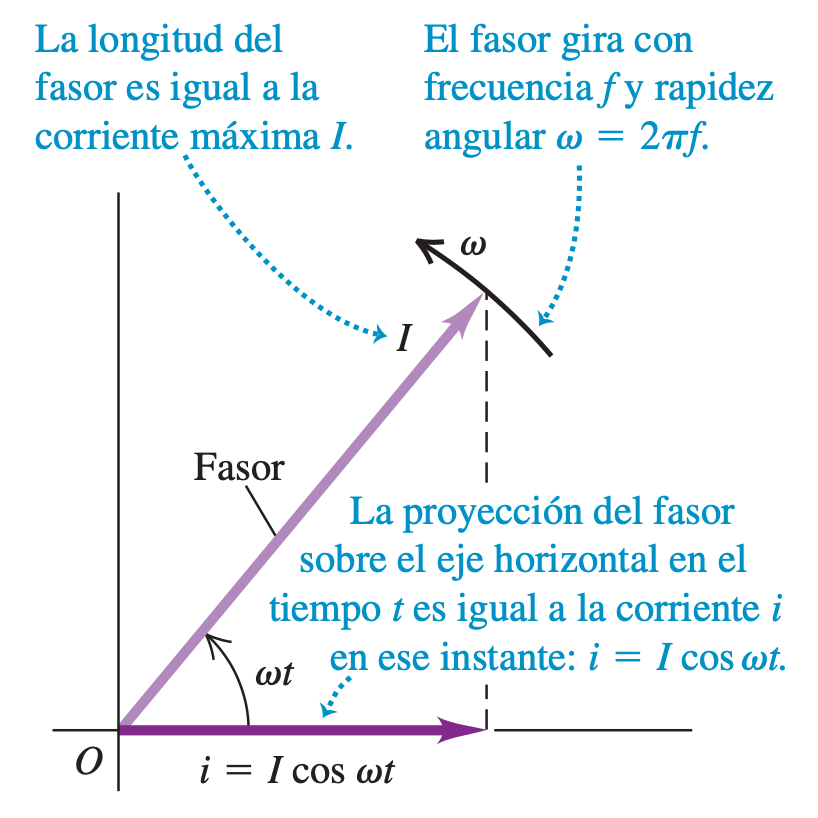
\includegraphics[scale=0.4]{fig/fasor1}
\caption{Diagrama de fasores}
\label{fig:fasor1}
\end{figure}











\chapter{Ondas electromagnéticas}
Las ecuaciones de Maxwell muestran que un campo magnético variable en el tiempo actúa como fuente de campo eléctrico, y que un campo eléctrico que varía con el tiempo genera un campo magnético. Estos campos $\vec{E}$ y $\vec{B}$ se sostienen uno al otro y forman una onda electromagnética que se propaga a través del espacio.

A diferencia de las ondas en una cuerda o las del sonido en un fluido, las ondas electromagnéticas no requieren un medio material.

\section{Ecuaciones de Maxwell y ondas electromagnéticas}
La ley de Faraday plantea que un campo magnético variable en el tiempo actúa como fuente de campo eléctrico, como lo demuestran las fem inducidas en los inductores y transformadores.

La ley de Ampère,  afirma que un campo eléctrico que cambia con el tiempo actúa como una fuente de campo magnético. Esta interacción mutua entre los dos campos se resume en las ecuaciones de Maxwell.

Así, cuando un campo, \textit{ya sea} eléctrico o magnético, cambia con el tiempo, induce un campo del otro tipo en las regiones adyacentes del espacio.

\subsection{Electricidad, magnetismo y luz}
Maxwell descubrió que los principios básicos del electromagnetismo podían expresarse en términos de las cuatro ecuaciones que hoy conocemos como \textbf{ecuaciones de Maxwell}. Estas cuatro ecuaciones son: 1) la ley de Gauss de los campos eléctricos; 2) la ley de Gauss de los campos magnéticos, que demuestra la inexistencia de monopolos magnéticos; 3) la ley de Ampère, que incluye la corriente de desplazamiento; y 4) la ley de Faraday:

\begin{equation}\label{29.18}\marginnote{Ley de Gauss}
\oint\vec{E}\cdot\, d\vec{A}=\frac{Q_{enc}}{\epsilon_0}
\end{equation}
\begin{equation}\label{29.19}\marginnote{Ley de Gauss del magnetismo}
\oint\vec{B}\cdot\, d\vec{A}=0
\end{equation}
\begin{equation}\label{29.20}\marginnote{Ley de Ampère}
\oint\vec{B}\cdot\, d\vec{l}=\mu_0\left(i_C+\epsilon_0\frac{d\Phi_E}{dt}\right)_{enc}
\end{equation}
\begin{equation}\label{29.21}\marginnote{Ley de Faraday}
\oint\vec{E}\cdot\, d\vec{l}=-\frac{d\Phi_B}{dt}
\end{equation}

Estas ecuaciones se aplican a los campos eléctricos y magnéticos \textit{en el vacío}. Si está presente un material, la permitividad $\epsilon_0$ y la permeabilidad $\mu_0$ del espacio libre se sustituyen por la permitividad $\epsilon$ y la permeabilidad $\mu$ del material. Si los valores de $\epsilon$ y $\mu$ son diferentes en puntos distintos en las regiones de integración, entonces $\epsilon$ y $\mu$ deben transferirse al lado izquierdo de (\ref{29.18}) y (\ref{29.20}), respectivamente, y colocarse dentro de las integrales. El término $\epsilon$ en (\ref{29.20}) también tiene que incluirse en la integral cuyo resultado es $d\Phi_B/dt$.

De acuerdo con las ecuaciones de Maxwell, una carga puntual en reposo produce
un campo $\vec{E}$ estático pero no un campo $\vec{B}$; una carga puntual en movimiento con velocidad constante produce los dos campos $\vec{E}$ y $\vec{B}$. Las ecuaciones de Maxwell también se usan para demostrar que para que una carga puntual produzca ondas electromagnéticas, la carga debe \textit{acelerar}. De hecho, un resultado general de las ecuaciones de Maxwell es que toda carga acelerada irradia energía electromagnética.

\subsection{Generación de la radiación electromagnética}
Una manera de conseguir que una carga puntual emita ondas electromagnéticas es haciéndola oscilar en movimiento armónico simple, de manera que tenga una aceleración casi en todo instante (excepto cuando la carga pasa por la posición de equilibrio).

Puesto que las perturbaciones eléctricas y magnéticas se dispersan o irradian desde la fuente, se utiliza de manera indistinta el nombre de \textbf{radiación electromagnética} o el de “ondas electromagnéticas”.

El físico alemán Heinrich Hertz, una vez que determinó la frecuencia de resonancia de sus circuitos, encontró la rapidez de las ondas a partir de la relación entre su longitud de onda y su frecuencia, $v=\lambda f$, y estableció que era igual a la rapidez de la luz. El valor moderno de la rapidez de la luz, que se denota con el símbolo $c$, es $299,792,458$ [m/s]. Para nuestros propósitos, el valor de $3.00 \times 10^8$ [m/s] tiene suficiente exactitud.

\subsection{El espectro electromagnético}
 El \textbf{espectro electromagnético} de las ondas electromagnéticas incluye las ondas de radio y televisión, la luz visible, la radiación infrarroja y ultravioleta, los rayos x y los rayos gamma.
 
A pesar de las muchas diferencias en su uso y medios de producción, todas ellas las ondas electromagnéticas tienen la misma rapidez de propagación (en el vacío), $c=299,792,458$ [m/s]. Las ondas electromagnéticas difieren en frecuencia $f$ y longitud de onda $\lambda$, pero la relación $c=\lambda f$ en el vacío se cumple para cada una.

Nosotros sólo podemos detectar directamente una parte muy pequeña del espectro con nuestro sentido de la vista, y a ese intervalo lo denominamos \textbf{luz visible}\footnote{La radiación electromagnética con la longitud de onda más corta, los rayos gamma, es producida en la naturaleza por los materiales radiactivos.}. Su intervalo de longitud de onda va de $400$ a $700$ nm ($400$ a $700\times 10^{-9}$ [m]), con frecuencias correspondientes de $750$ a $430$ THz ($7.5$ a $4.3\times 10^{14}$ [Hz]) aproximadamente.  Las distintas partes del espectro visible evocan en los humanos las sensaciones de los diferentes colores.

%\begin{figure}
%\centering
%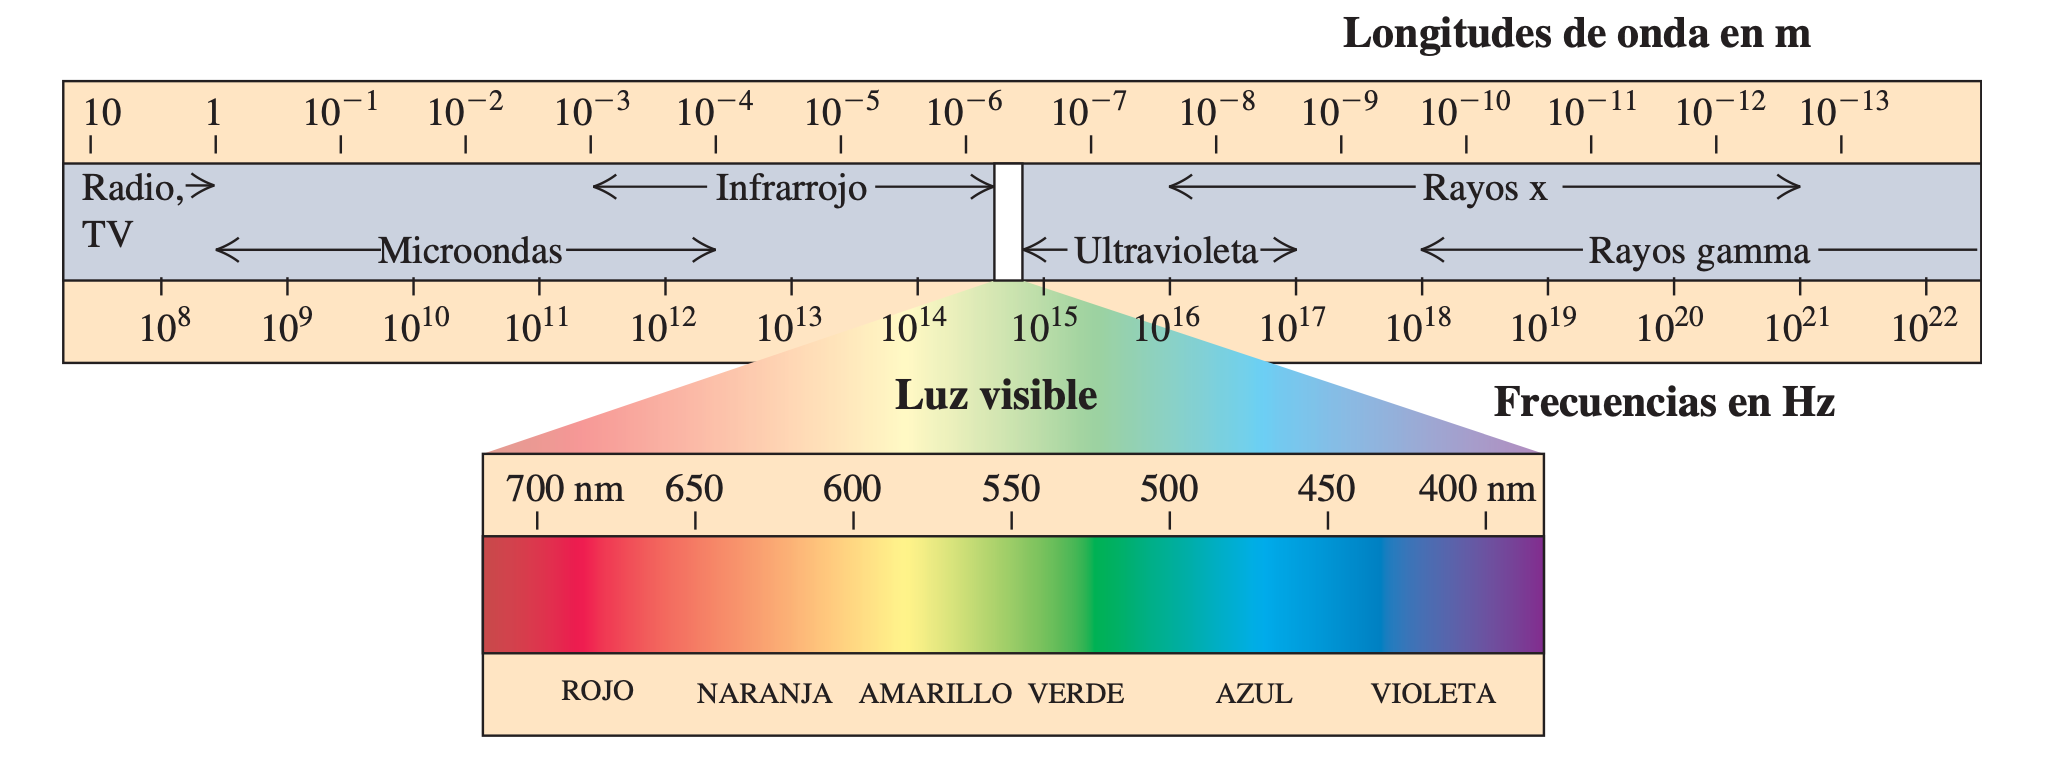
\includegraphics[scale=0.5]{fig/espectro}
%\caption{El espectro electromagnético. Las frecuencias y longitudes de onda que se encuentran en la naturaleza se extienden en un intervalo tan amplio que se tiene que usar una escala logarítmica para i%ndicar todas las bandas importantes. Las fronteras entre las bandas son un tanto arbitrarias.}
%\label{fig:espectro}
%\end{figure}

\section{Ondas electromagnéticas planas y rapidez de la luz}
Nuestro procedimiento consistirá en postular una configuración simple de campo eléctrico que tenga un comportamiento ondulatorio. Supondremos un campo eléctrico $\vec{E}$ que tenga sólo una componente $y$, y un campo magnético $\vec{B}$ sólo con una componente $z$, y supondremos que ambos campos se mueven juntos en la dirección $+x$ con una rapidez $c$ que al principio es desconocida

\subsection{Una onda electromagnética plana simple}

\begin{figure}[h]
\centering
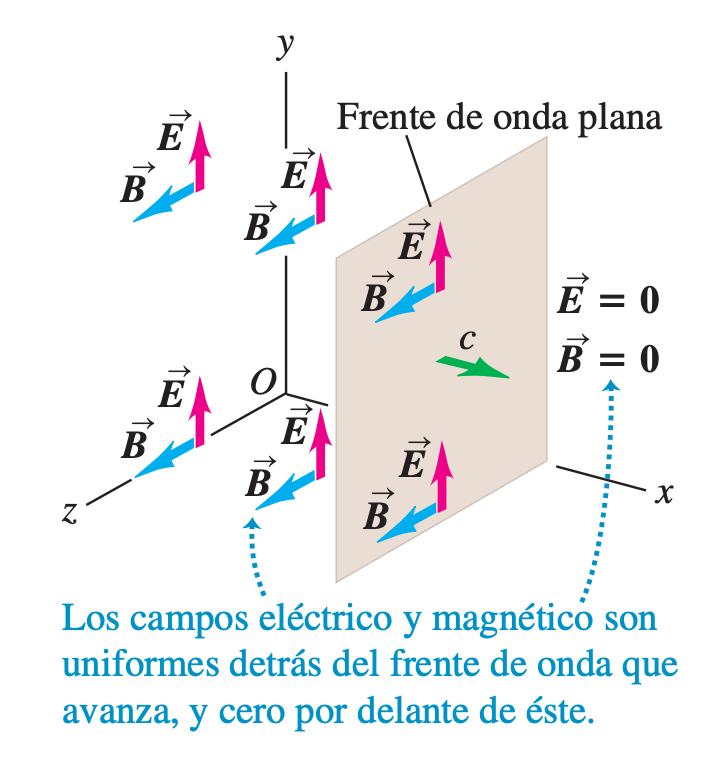
\includegraphics[scale=0.4]{fig/oeps}
\caption{Frente de una onda electromagnética.}
\label{fig:oeps}
\end{figure}

Si tomamos como base un sistema de coordenadas $xyz$ (figura \ref{fig:oeps}), suponemos que todo el espacio está dividido en dos regiones por un plano perpendicular al eje $x$ (y paralelo al plano $yz$). En cada punto a la izquierda de este plano hay un campo eléctrico uniforme $\vec{E}$ en la dirección $+y$ y un campo magnético uniforme $\vec{B}$ en la dirección $+z$, como se ilustra. Además supongamos que el plano limítrofe, al que llamaremos \textit{frente de onda}, se desplaza hacia la derecha en la dirección $+x$ con rapidez constante $c$, un valor que por el momento dejaremos indeterminado. Así, los campos $\vec{E}$ y $\vec{B}$ viajan a la derecha hacia regiones hasta ahora libres de campo con rapidez definida. En resumen, la situación describe una onda electromagnética rudimentaria. Una onda como ésta, en la que en cualquier instante los campos son uniformes en toda la extensión de cualquier plano perpendicular a la dirección de propagación, se llama \textbf{onda plana}. En el caso que se ilustra en la figura \ref{fig:oeps}, los campos son igual a cero para los planos que están a la derecha del frente de onda y tienen los mismos valores en todos los planos ubicados a la izquierda del frente de onda.

Verifiquemos si nuestra onda satisface la primera y segunda ecuaciones de Maxwell, es decir, las leyes de Gauss de los campos eléctrico y magnético. Para ello, tomaremos como nuestra superficie gaussiana una caja rectangular con lados paralelos a los planos coordenados $xy, xz$ y $yz$. La caja no encierra cargas eléctricas. Se puede demostrar que los flujos eléctrico y magnético totales a través de la caja son iguales a cero. Esto \textit{no} sería el caso si $\vec{E}$ o $\vec{B}$ tuvieran una componente $x$, paralela a la dirección de propagación. Así, para satisfacer las ecuaciones primera y segunda de Maxwell, los campos eléctrico y magnético deben ser perpendiculares a la dirección de propagación; es decir, la onda debe ser \textbf{transversal}.

La siguiente ecuación de Maxwell por considerar es la ley de Faraday:

\begin{equation}\label{32.1}
\oint\vec{E}\cdot\, d\vec{l}=-\frac{d\Phi_B}{dt}
\end{equation}

\begin{figure}[h]
\centering
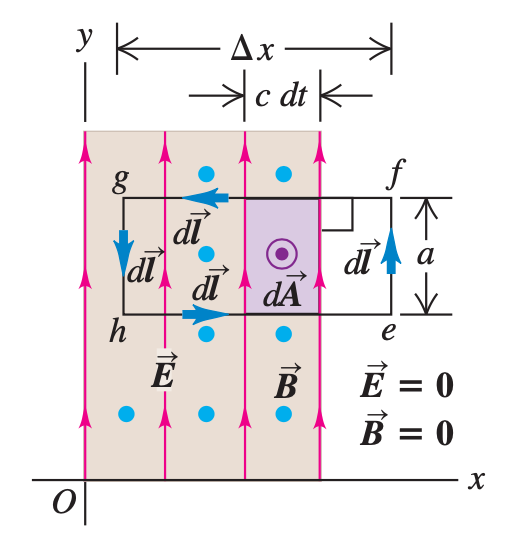
\includegraphics[scale=0.5]{fig/lf}
\caption{En el momento $dt$, el flujo magnético a través del rectángulo en el plano $xy$ se incrementa en una cantidad $d\Phi_B$. Este incremento es igual al flujo a través del rectángulo sombreado, con área $ac\, d$t; es decir, $d\Phi_B=Bac\, dt$. Por lo tanto, $d\Phi_B/dt=Bac$.}
\label{fig:lf}
\end{figure}

Para probar si nuestra onda satisface la ley de Faraday, aplicamos esta ley a un rectángulo $efgh$ paralelo al plano $xy$, el cual tiene altura $a$ y anchura $\Delta x$ (fugura \ref{fig:lf}). En el instante que se ilustra, el frente de onda ha avanzado parcialmente a través del rectángulo, y $\vec{E}$ es igual a cero a lo largo del lado $ef$. Al aplicar la ley de Faraday suponemos que el área vectorial $\vec{A}$ del rectángulo $efgh$ está en la dirección $+z$. Sólo el lado $gh$ contribuye a la integral, y sobre él $\vec{E}$ y $d\vec{l}$ son opuestos, por lo que se obtiene

\begin{equation}\label{32.2}
\oint\vec{E}\cdot\, d\vec{l}=-Ea
\end{equation}

Por consiguiente, el lado izquierdo de (\ref{32.2}) es diferente de cero.

Para satisfacer la ley de Faraday, (\ref{32.1}), debe haber una componente de $\vec{B}$ en la dirección $z$ (perpendicular a $\vec{E}$) de manera que pueda haber un flujo magnético $\Phi_B$ distinto de cero a través del rectángulo $efgh$ y una derivada $d\Phi_B/dt$ diferente de cero. En realidad, nuestra onda $\vec{B}$ tiene sólo la componente $z$. Durante un intervalo de tiempo $dt$, el frente de onda se desplaza una distancia $c\, dt$ hacia la derecha en la figura \ref{fig:lf}, y recorre un área $ac\, dt$ del rectángulo $efgh$. Durante este intervalo, el flujo magnético $\Phi_B$ a través del rectángulo $efgh$ se incrementa en $d\Phi_B =B(ac\, dt)$, por lo que la tasa de cambio del flujo magnético es

\begin{equation}\label{32.3}
\frac{d\Phi_B}{dt}=Bac
\end{equation}

Sustituyendo (\ref{32.2}) y (\ref{32.3}) en (\ref{32.1}), obtenemos

\begin{equation*}
-Ea=Bac
\end{equation*}
\begin{equation}\label{32.4}\marginnote{Onda electromagnética en el vacío}
\boxed{E=cB}
\end{equation}

Así, se ha demostrado que nuestra onda es congruente con la ley de Faraday sólo si su rapidez $c$ y las magnitudes de los vectores $\vec{E}$ y $\vec{B}$ guardan la relación que describe (\ref{32.4}).

Por último, se hace un cálculo similar empleando la ley de Ampère, el miembro restante de las ecuaciones de Maxwell. No hay corriente de conducción $(iC = 0)$, por lo que la ley de Ampère es

\begin{equation}\label{32.5}
\oint\vec{B}\cdot d\,\vec{l}=\mu_0\epsilon_0\frac{d\Phi_E}{dt}
\end{equation}

\begin{figure}[h]
\centering
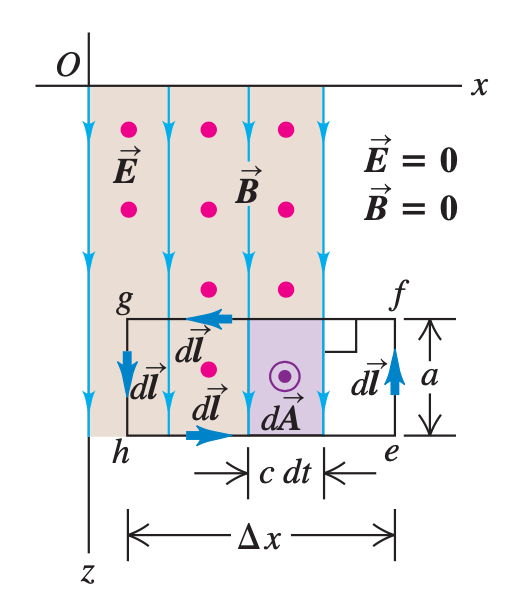
\includegraphics[scale=0.5]{fig/la}
\caption{Aplicación de la ley de Ampère
a una onda plana.}
\label{fig:la}
\end{figure}

Movemos nuestro rectángulo de manera que esté sobre el plano $xz$, como se ilustra en la figura \ref{fig:la}, y de nuevo observamos la situación en un momento en que el frente de onda haya viajado parcialmente a través del rectángulo. Tomamos el área vectorial $d\vec{A}$ en la dirección $+y$. Sólo el lado $gh$, donde $\vec{B}$ y $d\, \vec{l}$ son paralelos, contribuye a la integral, por lo que se obtiene

\begin{equation}\label{32.6}
\oint\vec{B}\cdot d\,\vec{l}=Ba
\end{equation}

Por consiguiente, el lado izquierdo de la ley de Ampère, (\ref{32.5}), es diferente de cero; el lado derecho también debe ser diferente de cero. Así, $\vec{E}$ debe tener una componente $y$ (perpendicular a $\vec{B}$) para que el flujo eléctrico $\Phi_E$ a través del rectángulo y la derivada con respecto al tiempo $d\Phi_E/dt$ puedan ser diferentes de cero. Llegamos
a la misma conclusión que inferimos a partir de la ley de Faraday: en una onda electromagnética, $\vec{E}$ y $\vec{B}$ deben ser perpendiculares entre sí.

En un intervalo de tiempo $dt$, el flujo eléctrico $\Phi_E$ a través del rectángulo se incrementa en $d\Phi_E =E(ac\, dt)$. La tasa de cambio eléctrico es

\begin{equation}\label{32.7}
\frac{d\Phi_E}{dt}=Eac
\end{equation}

Al sustituir las ecuaciones (\ref{32.6}) y (\ref{32.7}) en la ley de Ampère [\ref{32.5}], se encuentra

\begin{equation}\label{32.8}\marginnote{Onda electromagnética en el vacío}
\boxed{B=\epsilon_0\mu_0cE}
\end{equation}

De esta forma, la onda que hemos supuesto obedece la ley de Ampère sólo si la relación entre $B$, $c$ y $E$ es la que (\ref{32.8}).

Nuestra onda electromagnética debe obedecer tanto la ley de Ampère como la de Faraday, de manera que (\ref{32.4}) y (\ref{32.8}) deben satisfacerse. Esto sólo ocurre si $\epsilon_0\mu_0c= 1/c$, o:

\begin{equation}\label{32.9}\marginnote{Rapidez de las ondas electromagnéticas en el vacío}
\boxed{c=\frac{1}{\sqrt{\epsilon_0\mu_0}}}
\end{equation}

Al sustituir los valores numéricos de estas cantidades, encontramos que $$c=3.00\times 10^8 \textup{m/s}$$

La onda que supusimos es congruente con todas las ecuaciones de Maxwell, siempre y cuando su frente de onda se desplace con la rapidez indicada, la cual reconocemos de inmediato como ¡la rapidez de la luz!

\subsection{Propiedades clave de las ondas electromagnéticas}
Para nuestro estudio elegimos una onda simple con la finalidad de evitar complicaciones matemáticas, pero este caso especial ilustra varias características importantes de \textit{todas} las ondas electromagnéticas:
\begin{enumerate}
\item La onda es \textit{transversal}; tanto $\vec{E}$ como $\vec{B}$ son perpendiculares a la dirección de propagación de la onda. Los campos eléctrico y magnético también son perpendiculares entre sí. La dirección de propagación es la dirección del producto vectorial $\vec{E}\times\vec{B}$.
\item Hay una razón definida entre las magnitudes de $\vec{E}$ y $\vec{B}$: $E = cB$.
\item La onda viaja en el vacío con rapidez definida e invariable.
\item A diferencia de las ondas mecánicas, que necesitan de partículas oscilantes de un medio para transmitirse, las ondas electromagnéticas no requieren un medio. Lo que “ondula” en una onda electromagnética son los campos eléctricos y magnéticos.
\end{enumerate}

Se dice que una onda en la que $\vec{E}$ siempre es paralelo a cierto eje está \textbf{polarizada linealmente} a lo largo de ese eje. Más en general, cualquier onda que viaje en la dirección $x$ se puede representar como una superposición de ondas polarizadas linealmente en las direcciones $y$ y $z$.

%\subsection{*Deducción de la ecuación de onda electromagnética}
%A continuación se presenta otra deducción de la ecuación \ref{32.9} que describe la rapidez de las ondas electromagnéticas.

\section{Ondas electromagnéticas sinusoidales}
En una onda electromagnética sinusoidal, $\vec{E}$ y $\vec{B}$ en cualquier punto del espacio son funciones sinusoidales del tiempo, y en cualquier instante la variación \textit{espacial} de los campos también es sinusoidal.

La frecuencia $f$, la longitud de onda $\lambda$ y la rapidez de propagación $c$ de cualquier onda periódica guardan entre sí la conocida relación entre longitud de onda y frecuencia, $c=\lambda f$.

\subsection{Campos de una onda sinusoidal}

\begin{figure}[h]
\centering
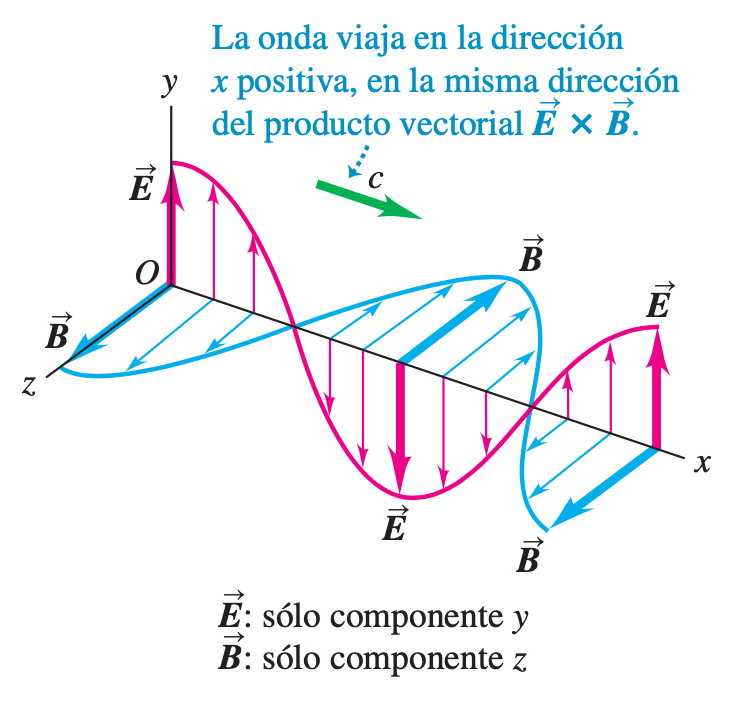
\includegraphics[scale=0.5]{fig/sinusoidal}
\caption{Representación de los campos eléctricos y magnéticos como funciones de x correspondientes a una onda electromagnética sinusoidal plana linealmente polarizada. Se ilustra una longitud de onda de la onda en el tiempo $t = 0$. Los campos se indican sólo para puntos a lo largo del eje $x$.}
\label{fig:sinusoidal}
\end{figure}

La figura \ref{fig:sinusoidal} muestra una onda electromagnética polarizada sinusoidal que viaja en la dirección $+x$. Observe que los campos eléctrico y magnético oscilan en fase: $\vec{E}$ es máximo donde $\vec{B}$ también lo es, y $\vec{E}$ es igual a cero donde $\vec{B}$ también vale cero. Advierta también que donde $\vec{E}$ está en la dirección $+y$, $\vec{B}$ tiene la dirección $+z$; y donde $\vec{E}$ está en la dirección $-y$, $\vec{B}$ está en la dirección $-z$. En todos los puntos, el producto vectorial $\vec{E}\times\vec{B}$ está en la dirección en que se propaga la onda .\footnote{En realidad, en una onda plana sinusoidal hay campos eléctricos y magnéticos en todos los puntos del espacio}.

Podemos describir las ondas electromagnéticas por medio de \textit{funciones de onda}, similar a como se hace para el caso de las ondas de una cuerda (ver sección \ref{cap:funcion-de-onda}). La ecuación (\ref{15.7}) es una forma de la función de onda para una onda transversal que viaja en la dirección $+x$ a lo largo de una cuerda estirada:

\begin{equation*}
y(x,t)=A\cos (kx-\omega t)
\end{equation*}

Dejemos que $E_y(x, t)$ y $B_z(x, t)$ representen los valores instantáneos de la componente $y$ de $\vec{E}$ y la componente $z$ de $\vec{B}$ en la figura \ref{fig:sinusoidal}, y sea que $E_{max}$ y $B_{max}$ representen los valores máximos, o amplitudes, de estos campos. De esta forma, las funciones de onda para la onda son

\begin{equation}\label{32.16}\marginnote{Onda electromagnética sinusoidal plana que se propaga en la dirección $+x$}
E_y(x,t)=E_{max}\cos (kx-\omega t)\qquad B_z(x,t)=B_{max}\cos (kx-\omega t)
\end{equation}

También es posible escribir las funciones de onda en forma vectorial:

\begin{equation}\label{32.17}
\boxed{\vec{E}(x,t)=\hat{j}E_{max}\cos (kx-\omega t)\qquad \vec{B}(x,t)=\hat{k}B_{max}\cos (kx-\omega t)}
\end{equation}

De (\ref{32.4}) se desprende que las amplitudes deben estar relacionadas mediante la expresión

\begin{equation}\label{32.18}\marginnote{Onda ekectromagnética en el vacío}
\boxed{E_{max}=cB_{max}}
\end{equation}

\begin{figure}
\centering
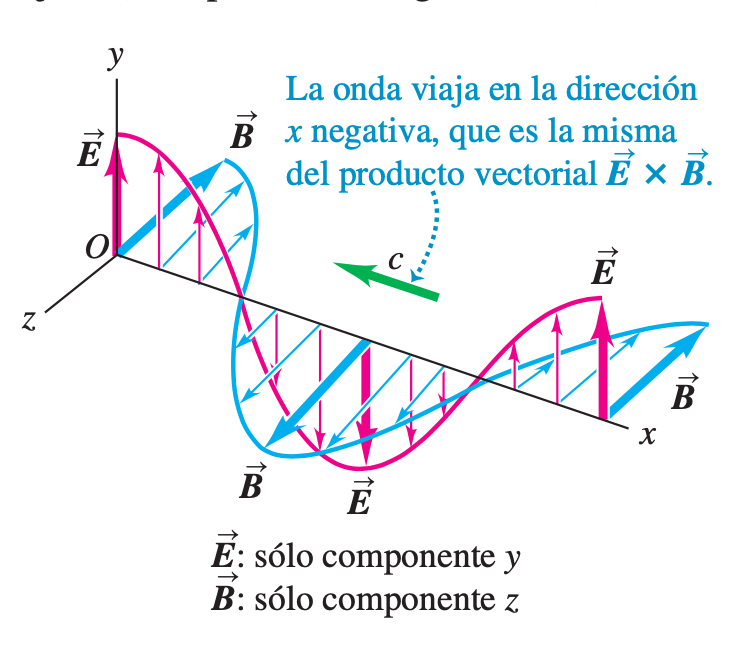
\includegraphics[scale=0.5]{fig/sinusoidal2}
\caption{Representación de una longitud de onda de una onda electromagnética sinusoidal plana linealmente polarizada, que viaja en la dirección $x$ negativa en el instante $t = 0$.}
\label{fig:sinusoidal2}
\end{figure}

La figura \ref{fig:sinusoidal2} muestra los campos eléctrico y magnético de una onda que viaja en la dirección $x$ negativa. Las funciones de onda correspondientes a esta onda son

\begin{equation}\label{32.19}\marginnote{Onda electromagnética sinusoidal plana, que se propaga en la dirección $-x$}
E_y(x,t)=E_{max}\cos (kx+\omega t)\qquad B_z(x,t)=-B_{max}\cos (kx+\omega t)
\end{equation}

\section{Energía y cantidad de movimiento de las ondas electromagnéticas}
Es un hecho muy conocido que hay energía asociada con las ondas electromagnéticas; piense en la energía de la radiación solar. 

Sabemos que en una región de espacio vacío donde están presentes los campos $\vec{E}$ y $\vec{B}$ la densidad total de energía $u$ está dada por

\begin{equation}\label{32.23}
u=\frac{1}{2}\epsilon_0E^2+\frac{1}{2\mu_0}B^2
\end{equation}

Para las ondas electromagnéticas en el vacío, las magnitudes $E$ y $B$ están relacionadas por

\begin{equation}\label{32.24}
B=\frac{E}{c}=\sqrt{\epsilon_0\mu_0}E
\end{equation}

Al combinar (\ref{32.23}) y (\ref{32.24}) también se puede expresar la densidad de energía $u$ en una onda electromagnética simple en el vacío como

\begin{equation}\label{32.25}
u=\frac{1}{2}\epsilon_0E^2+\frac{1}{2\mu_0}(\sqrt{\epsilon_0\mu_0}E)^2=\epsilon_0E^2
\end{equation}

Esto demuestra que en el vacío, la densidad de energía asociada con el campo $\vec{E}$ en nuestra onda simple es igual a la densidad de energía del campo $\vec{B}$. En general, la magnitud del campo eléctrico $E$ es función de la posición y el tiempo, igual que para la onda sinusoidal descrita por las ecuaciones (\ref{32.16}); así, la densidad de energía $u$ de una onda electromagnética, dada por la ecuación (\ref{32.25}), también depende en general de la posición y el tiempo.

\subsection{Flujo de energía electromagnética y el vector de Poynting}
Las ondas electromagnéticas como las que hemos descrito son ondas que \textit{viajan} y transportan energía de una región a otra. Esta transferencia de energía se puede describir en términos de la energía transferida \textit{por unidad de tiempo por unidad de área de sección transversal, o potencia por unidad de área}, para un área perpendicular a la dirección en que viaja la onda.

\begin{figure}
\begin{center}
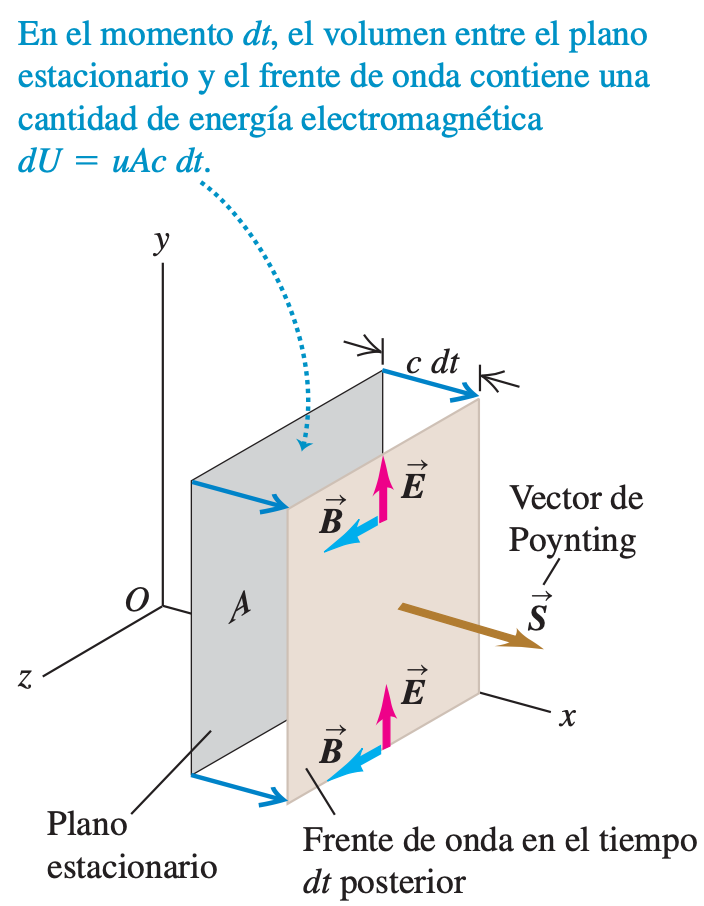
\includegraphics[scale=0.5]{fig/3217}
\caption{Frente de onda en el momento $dt$ después de haber pasado a través del plano estacionario con área $A$}
\label{fig:32.17}
\end{center}
\end{figure}


Para ver cómo se relaciona el flujo de energía con los campos, considere un plano estacionario, perpendicular al eje $x$, que coincida con el frente de onda en cierto momento. En un tiempo dt después de eso, el frente de onda se desplaza una distancia $dx = c\, dt$ hacia la derecha del plano. Si se considera un área $A$ sobre este plano estacionario (figura \ref{fig:32.17} ), advertimos que la energía del espacio a la derecha de esta área debió haber pasado a través del área para llegar a la nueva ubicación. El volumen $dV$ de la región en cuestión es el producto del área de la base $A$ por la longitud $c\, dt$, y la energía $dU$ de esta región es el producto de la densidad de energía $u$ por este volumen: $$dU=u\, dV=(\epsilon_0E^2)(Ac\, dt)$$

Esta energía pasa a través del área $A$ en el tiempo $dt$. El flujo de energía por unidad de
tiempo por unidad de área, que llamaremos $S$, es

\begin{equation}\label{32.26}
S=\frac{1}{A}\frac{dU}{dt}=\epsilon_0cE^2 \qquad \mbox{(en el vacío)}
\end{equation}

Las unidades de $S$ son energía por unidad de tiempo por uniad de área, o potencia por unidad de área.

Es posible definir una cantidad \textit{vectorial} que describa tanto la magnitud como la dirección de la tasa del flujo de energía:

\begin{equation}\label{32.28}\marginnote{Vector de Poynting en el vacío}
\boxed{\vec{S}=\frac{1}{\mu_0}\vec{E}\times\vec{B}}
\end{equation}

El vector $\vec{S}$ se denomina \textbf{vector de Poynting}. Su dirección es la misma en que se propaga la oinda. Como $\vec{E}$ y $\vec{B}$ son perpendiculares, la magnitud de $\vec{S}$ es $S=EB/\mu_0$; según (\ref{32.26}), éste es el flujo de energía por unida de área y por unidad de tiempo a través de un área de sección trnasversal perpendicular a la dirección de propagación. El flujo total de energía por uniad de tiempo (potencia $P$) hacia fiera de cualquier superficie cerrada es la integral de $\vec{S}$ sobre la superficie: $$P=\oint \vec{S}\cdot d\vec{A}$$. 

En el caso de las ondas sinosoidales, los campos eléctricos y masgnéticos en un ounto cualquiera varían en el tiempo, por lo que el vector de Poynting en cualquier punto también es función del tiempo. Puesto que las frecuencias de las ondas electromagnéticas comunes son muy altas, la variación en el tiempo del vector Poynting es tan rápida que lo más apropiado es examinar su valor \textit{medio}. La magnitud del valor medio de $\vec{S}$ en un punto recibe el nombre de \textbf{intensidad} de la radiación en ese punto. Veamos cuál es la intensiad de la onda sinosoidal descrita por (\ref{32.17}). Primero sustituimos $\vec{E}$ y $\vec{B}$ en (\ref{32.28}):

\begin{align*}
\vec{S}(x,t)&=\frac{1}{\mu_0}\vec{E}(x,t)\times\vec{B}(x,t) \\
&=\frac{1}{\mu_0}[\hat{j}E_{max}\cos(kx-\omega t)]\times [\hat{k}B_{max}\cos(kx-\omega t)]
\end{align*}

El producto vectorial de los vectores unitarios $\hat{j}\times \hat{k}=\hat{i}$, y $\cos^2(kx-\omega t)$ nunca es negativo, por lop que $\vec{S}(x,t)$ siemore apunta en la dirección $x$ positiva (la dirección de propagación de la onda). La componente $x$ del vector de Poynting es

\begin{equation*}
S_x(x,t)=\frac{E_{max}B_{max}}{\mu_0}\cos^2(kx-\omega t)=\frac{E_{max}B_{max}}{2\mu_0}[1+\cos 2(kx-\omega t)]
\end{equation*}

El valor medie del tiempo de $\cos 2(kx-\omega t)$ es igual a cero porque, en cualquier punto, es positivo durante la mitad de un ciclo y negtivo durante la otra mitad. Por lo tanto, el valor medio del vector de Poynting en un ciclo completo es $\vec{S}_{med}=\hat{i}S_{med}$, donde $$S_{med}=\frac{E_{max}B_{max}}{2\mu_0}$$

Es decir, la magnitud del valor medio de $\vec{S}$ para una onda siusoidal (la intensidad $I$ de la onda) es $\frac{1}{2}$ del valor máximo. Con base en las relaciones $E_{max}=B_{max}c$ y $\epsilon_0\mu_0=1/c^2$, podemos expresar la intensidad en varias formas equivalentes:

\begin{align*}\label{32.29}\marginnote{Intensidad de una onda sinusoidal en el vacío}
I&=S_{med}=\frac{E_{max}B_{max}}{2\mu_0}=\frac{E^2_{max}}{2\mu_0} \\
&=\frac{1}{2}\sqrt{\frac{\epsilon_0}{\mu_0}}E^2_{max}=\frac{1}{2}\epsilon_0cE^2_{max}
\end{align*}

Se invita al lectro a que compruebe que es estas expresiones son equivalentes.

En el caso de una onda que viaja en la dirección $-x$, el vector de Poynting tiene la dirección $-x$ en todos los puntos, pero su magnitud es la misma que en el caso de una onda que viaja en la dirección $+x$.

A lo largo de este análisis hemos considerado sólo ondas electromagnéticas que se propagan en el vacío. Sin embargo, si las ondas viajan en un medio dieléctrico, debem modificarse las expresiones para densidad de energía [(\ref{32.23})], el vector de Poynting [(\ref{32.28})] y la intensidad de una onda sinusoidal [(\ref{32.29})]. Los cambios requeridos son muy sencillos: basta con sustituir $\epsilon_0$ por la permitividad $\epsilon$ del dieléctrico, $\mu_0$ por la permitividad $\mu$ del dieléctrico, y $c$ por la rapidez $v$ de las ondas electromagnéticas en el dieléctrico. De manera sorpendente, las densidades de energía en los campo $\vec{E}$ y $\vec{B}$ son iguales incluso en un dieléctrico.






















\appendix
\chapter{Ondas periódicas}\label{cap:funcion-de-onda}
\section{Ondas transversales periódicas}
En particular, suponga que movemos verticalmente la cuerda con un \textit{movimiento armónico simple} (MAS) con amplitud $A$, frecuencia $f$, frecuencia angular $\omega=2\pi f$, y periodo $T = 1/f = 2\pi/\omega$. Las ondas periódicas con movimiento armónico simple las llamamos \textbf{ondas senoidales}. Resulta también que \textit{cualquier} onda periódica puede representarse como una combinación de ondas senoidales.\footnote{No confunda el movimiento de la onda transversal a lo largo de la cuerda con el de una partícula de la cuerda. La onda avanza con rapidez constante v a lo largo de la cuerda; mientras que el movimiento de la partícula es armónico simple y transversal (perpendicular) a la longitud de la cuerda.}

\begin{quote}
Cuando una onda senoidal pasa por un medio, todas las partículas del medio sufren movimiento armónico simple con la misma frecuencia.
\end{quote}

La longitud de un patrón de onda completo es la distancia entre una cresta y la siguiente, o de un valle al siguiente, o de cualquier punto al punto correspondiente en la siguiente repetición de la forma. Llamamos a esta distancia \textbf{longitud de onda}, denotada con $\lambda$. El patrón de onda viaja con rapidez constante $v$ y avanza una longitud de onda $\lambda$ en el lapso de un periodo $T$. Por lo tanto, la rapidez de la onda $v$ está dada por $v = \lambda /T$, dado que $f = 1/T$,

\begin{equation}\label{15.1}\marginnote{Onda periódica}
\boxed{v=\lambda f}
\end{equation}

\section{Descripción matemática de una onda}
Necesitamos el concepto de \textit{función de onda}, una función que describe la posición de cualquier partícula en el medio en cualquier instante. Nos concentraremos en las ondas \textit{senoidales}, en las que cada partícula tiene un MAS alrededor de su posición de equilibrio.

Como ejemplo específico, examinemos las ondas en una cuerda estirada. Si despreciamos el pandeo de la cuerda por la gravedad, su posición de equilibrio es en una línea recta, la cual tomamos como el eje $x$ de un sistema de coordenadas. Las ondas en una cuerda son transversales; durante el movimiento ondulatorio una partícula con posición de equilibrio $x$ se desplaza cierta distancia y en la dirección perpendicular al eje $x$. El valor de $y$ depende de cuál partícula estamos considerando (es decir, y depende de $x$) y también del instante $t$ en que la consideramos. Así, y es función tanto de $x$ como de $t$; $y = y(x, t)$. Llamamos a $y(x, t)$ la \textbf{función de onda} que describe la onda. Con esto podemos calcular la velocidad y la aceleración de cualquier partícula, la forma de la cuerda y todo lo que nos interese acerca del comportamiento de la cuerda en cualquier instante.

\subsection{Función de onda de una onda senoidal}
Supongamos que una onda senoidal viaja de izquierda a derecha (dirección de $x$ creciente) por la cuerda. Cada partícula de la cuerda oscila en movimiento armónico simple con la misma amplitud y frecuencia; pero las oscilaciones de partículas en diferentes puntos de la cuerda \textit{no} están todas coordinadas. 

Los movimientos cíclicos de diversos puntos de la cuerda están desfasados entre sí en diversas fracciones de un ciclo. Llamamos a éstas \textit{diferencias de fase}, y decimos que la \textit{fase} del movimiento es diferente para diferentes puntos. Por ejemplo, si un punto tiene su desplazamiento positivo máximo al mismo tiempo que otro tiene su desplazamiento negativo máximo, los dos están desfasados medio ciclo.

Suponga que el desplazamiento de una partícula en el extremo izquierdo de la cuerda ($x = 0$), donde la onda se origina, está dado por

\begin{equation}\label{15.2}
y(x=0,t)=A\cos\omega t=A\cos 2\pi ft
\end{equation}

En $t = 0$, la partícula en $x =0$ tiene máximo desplazamiento positivo ($y = A$) y está instantáneamente en reposo (porque el valor de $y$ es un máximo).

La perturbación ondulatoria viaja de $x = 0$ a algún punto $x$ a la derecha del origen en un tiempo dado por $x/v$, donde $v$ es la rapidez de la onda. Así, el movimiento del punto $x$ en el instante $t$ es el mismo que el movimiento del punto $x = 0$ en el instante anterior $t - x/v$. Por lo tanto, podemos obtener el desplazamiento del punto $x$ en el instante $t$ con sólo sustituir $t$ en (\ref{15.2}) por $(t - x/v)$. Al hacerlo, obtenemos la siguiente expresión para la función de onda:

\begin{equation*}
y(x,t)=A\cos \left[\omega\left(t-\frac{x}{v}\right)\right]
\end{equation*}

Dado que $\cos (-\theta) = \cos \theta$, podemos rescribir la función de onda así:

\begin{equation}\label{15.3}\marginnote{Onda senoidal que avanza en la dirección $+x$}
\boxed{y(x,t)=A\cos \left[\omega\left(\frac{x}{v}-t\right)\right]=A\cos 2\pi f\left(\frac{x}{v}-t\right)}
\end{equation}

Podemos rescribir la función de onda dada por (\ref{15.3}) de varias formas distintas pero útiles. Una es expresarla en términos del periodo $T = 1/f$ y la longitud de onda $\lambda = v/f$:

\begin{equation}\label{15.4}\marginnote{Onda senoidal que se mueve en la dirección $+x$}
\boxed{y(x,t)=A\cos 2\pi\left(\frac{x}{\lambda}-\frac{t}{T}\right)}
\end{equation}

Obtenemos otra forma útil de la función de onda, si definimos una cantidad $k$ llamada \textbf{número de onda}\footnote{Algunos físicos definen el número de onda como $1/\lambda$ en vez de $2\pi/\lambda$. Al leer otros textos, verifique cómo se definió este término.}

\begin{equation}\label{15.4}\marginnote{Número de onda}
k=\frac{2\pi}{\lambda}
\end{equation}

Sustituyendo $\lambda = 2\pi /k$ y $f = \omega /2\pi$ en la relación longitud de onda-frecuencia $v =\lambda f$ obtenemos

\begin{equation}\label{15.6}\marginnote{Onda periódica}
\omega = vk
\end{equation}

Reescribiendo (\ref{15.4})

\begin{equation}\label{15.7}\marginnote{Onda senoidal que se mueve en la dirección $+x$}
\boxed{y(x,t)=A\cos (kx-\omega t)}
\end{equation}

\subsection{Más acerca de la función de onda}
Podemos modificar (\ref{15.3}) a (\ref{15.7}) para representar una onda que viaja en la dirección $x$ negativa. En este caso, el desplazamiento del punto $x$ en el instante $t$ es el mismo que el del punto $x=0$ en un instante posterior $(t + x/v)$. Sustituyendo en (\ref{15.2})

\begin{equation}\label{15.8}\marginnote{Nnda senoidal que se mueve en la dirección $-x$}
y(x,t)=A\cos 2\pi f\left(\frac{x}{v}+t\right)=A\cos 2\pi \left(\frac{x}{\lambda}+\frac{t}{T}\right)=A\cos (kx+\omega t)
\end{equation}

En la expresión $y(x, t) =A\cos (kx \pm vt)$ para una onda que viaja en la dirección $-x$ o bien $+x$, la cantidad $(kx \pm vt)$ se denomina \textbf{fase}, y desempeña el papel de cantidad angular en (\ref{15.7}) y (\ref{15.8}); su valor para cualesquiera valores de $x$ y $t$ determina qué parte del ciclo senoidal existe en un punto e instante dados.

La rapidez de onda es la rapidez con que tenemos que movernos con la onda para mantenernos junto a un punto que tiene una fase dada, como una cresta específica de una onda en una cuerda. Para una onda que viaja en la dirección $+x$, eso implica $kx - vt =$ constante. Derivando con respecto a t, $$\frac{dx}{dt}=\frac{\omega}{k}$$

\subsection{Velocidad y aceleración de partículas en una onda senoidal}
De la función de onda podemos obtener una expresión para la velocidad transversal de cualquier \textit{partícula} en una onda transversal, que llamaremos $v_y$ para distinguirla de la rapidez de propagación de la onda, $v$. Si la función de onda es $$y(x,t)=A\cos (kx-\omega t)$$ entonces,

\begin{equation}\label{15.9}
v_y(x,t)=\frac{\partial y(x,t)}{\partial t}=\omega A\sin (kx-\omega t)
\end{equation}
 (\ref{15.9}) muestra que la velocidad transversal de una partícula varía con el tiempo.
 
La \textit{aceleración} de cualquier partícula es la segunda derivada parcial de $y(x, t)$ con respecto a $t$:

\begin{equation}\label{15.10}
a_y(x,t)=\frac{\partial ^2y(x,t)}{\partial t^2}=-\omega ^2A\cos (kx-\omega t)=-\omega ^2y(x,t)
\end{equation}

También podemos calcular derivadas parciales de $y(x, t)$ con respecto a $x$, manteniendo $t$ constante. Esto equivale a estudiar la forma de la cuerda en un momento dado, como una fotografía instantánea. La primera derivada $\partial y(x,t)/\partial x$ es la \textit{pendiente} de la cuerda en cualquier punto. La segunda derivada parcial con respecto a $x$ es la \textit{curvatura} de la cuerda:

\begin{equation}\label{15.11}
\frac{\partial ^2y(x,t)}{\partial x^2}=-k^2A\cos (kx-\omega t)=-k^2y(x,t)
\end{equation}

Por (\ref{15.10}) y (\ref{15.11}), y la relación $\omega = vk$, vemos que

\begin{equation*}
\frac{\partial ^2(x,t)/\partial t^2}{\partial ^2y(x,t)/\partial x^2}=\frac{\omega^2}{k^2}=v^2
\end{equation*}
y
\begin{equation}\label{15.12}\marginnote{Ecuación de onda}
\boxed{\frac{\partial ^2y(x,t)}{\partial x^2}=\frac{1}{v^2}\frac{\partial^2y(x,t)}{\partial t^2}}
\end{equation}

Se pueden seguir los mismos pasos para demostrar que la función de onda para una onda senoidal que se propaga en la dirección $x$ negativa, también satisface (\ref{15.12}). Esta ecuación, llamada \textbf{ecuación de onda}, es una de las más importantes en física. Siempre que ocurre, sabemos que una perturbación puede propagarse como onda a lo largo del eje $x$ con rapidez $v$. La perturbación no tiene que ser una onda senoidal; \textit{cualquier} onda en una cuerda obedece la ecuación (\ref{15.12}), sea periódica o no.
























\newpage
\begin{thebibliography}{}
\bibitem{Libro1}YOUNG, HUGH D. y ROGER A. FREEDMAN. (2009). \textit{Física universitaria volumen 1. Decimosegunda edición}. PEARSON EDUCACIÓN.
\bibitem{Libro2} YOUNG, HUGH D. y ROGER A. FREEDMAN. (2009). \textit{Física universitaria, con física moderna volumen 2.
Decimosegunda edición}. PEARSON EDUCACIÓN.

\end{thebibliography}

\end{document}

\chapter{Potencial eléctrico }
Cuando una partícula con carga se mueve en un campo eléctrico, el campo ejerce una fuerza que efectúa \textit{trabajo} sobre la partícula. Este trabajo siempre se puede expresar en términos de la energía potencial eléctrica\footnote{O simplemente \textit{potencial eléctrico} o \textit{potencial}}. Una diferencia de potencial entre un punto y otro reciba el nombre de \textit{voltaje}.

\section{Energía potencial eléctrica}
Cuando una fuerza $\vec{F}$ actúa sobre una partícula que se mueve de un punto $a$ a un punto $b$, el trabajo $W_{a\to b}$ efectuado por la fuerza está dado por la siguiente \textit{integral de línea}:

\begin{equation}\label{23.1}\marginnote{Trabajo realizado por una fuerza}
W_{a\to b}=\int_a^b\vec{F}\cdot d\vec{l}=\int_a^bF\cos\phi dl
\end{equation}

donde $d\vec{l}$ es un desplazamiento infinitisimal a lo largo de la trayectoria de la partícula, y $\phi$ es el ángulo entre $\vec{F}$ y $d\vec{l}$ 	en cada punto de la trayectoria.

Si la fuerza $\vec{F}$ es \textit{conservativa}, el trabajo realizado por esta siempre se puedo expresar en términos de una \textbf{energía potencial} $U$. Cuando la partícula se mueve de un punto donde la energía potencial es $U_a$ a otro donde es $U_b$, el cambio de energía potencial es $\Delta U=U_b-U_a$, y el trabajo $W_{a\to b}$ que realiza la fuerza es

\begin{equation}\label{23.2}\marginnote{Trabajo efectuado por una fuerza conservativa}
\boxed{W_{a\to b}=U_a-U_b=-(U_b-U_a)=-\Delta U}
\end{equation}

En tercer lugar, el teorema del trabajo y la energía establece que el cambio en la energía cinética $\Delta K=K_b+K_a$ durante cualquier desplazamiento es igual al trabajo \textit{total} realizado sobre la partícula. Si el único trabajo efectuado sobre la partícula lo realizan fuerzas conservativas, entonces la ecuación \ref{23.2} da el trabajo total, y $K_b-K_a=-(U_b-U_a)$. Es decir, 

\begin{equation}\label{23.3}
K_a+U_a=K_b+U_b
\end{equation}

Es decir, en estas circunstancias, la energía mecánica total (cinética más potencial) se
\textit{conserva}.

\subsection{Energía potencial eléctrica de un campo uniforme}
\begin{figure}[h]
\centering
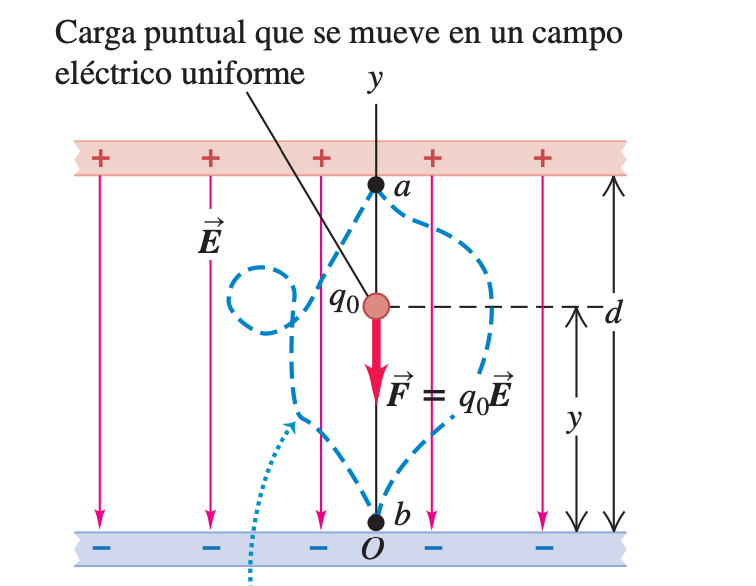
\includegraphics[scale=0.5]{fig/energia_potencial}
\caption{Trabajo realizado sobre una carga puntual que se mueve en un campo eléctrico uniforme. El trabajo realizado por la fuerza eléctrica es el mismo para cualquier trayectoria de $a$ a $b$: $W_{a\to b}=-\Delta U=q_0Ed$} 
\label{fig:energia_potencial}
\end{figure}

En la figura \ref{fig:energia_potencial} un par de placas metálicas paralelas con carga generan un campo eléctrico uniforme descendente y con magnitud $E$. El campo ejerce una fuerza hacia abajo con magnitud $F=q_0E$ sobre una carga de prueba positiva $q_0$. A medida que la carga se mueve hacia abajo una distancia $d$ del punto $a$ al punto $b$, la fuerza sobre la carga de prueba es constante e independiente de su localización. Por lo tanto, el trabajo realizado por el campo eléctrico es 

\begin{equation}\label{23.4}
W_{a\to b}=Fd=q_0Ed
\end{equation}

Este trabajo es positivo, toda vez que la fuerza está en la misma dirección que el desplazamiento neto de la carga de prueba. Este trabajo puede representarse con una función de \textbf{energía potencial} $U$, que para la fuerza eléctrica está dada por

\begin{equation}\label{23.5}
U=q_0Ey
\end{equation}

Cuando la carga de prueba se mueve de la altura $y_a$ a la altura $y_b$, el trabajo realizado sobre la carga por el campo está dado por

\begin{equation}\label{23.6}
W_{a\to b}=-\Delta U=-(U_b-U_a)=-(q_0Ey_b-q_0Ey_a)=q_0E(y_a-y_b)
\end{equation}

\subsection{Energía potencial entre dos cargas puntuales}
El concepto de energía potencial se puede aplicar a una carga puntual en \textit{cualquier} campo eléctrico generado por una distribución de carga estática. 
Cualquier distribución de carga se representa como un conjunto de cargas puntuales. Por consiguiente, es útil calcular el trabajo realizado sobre una carga de prueba $q_0$ que se mueve en el campo eléctrico ocasionado por una sola carga puntual estacionaria $q$.

En primer lugar se considerará un desplazamiento a lo largo de una línea radial, del punto $a$ al punto $b$. La fuerza sobre $q_0$ está dada por la ley de Coulomb, y su componente radial es

\begin{equation}\label{23.7}
F_r=\frac{1}{4\pi\epsilon_0}\frac{qq_0}{r^2}
\end{equation}

Si $q$ y $q_0$ tienen el mismo signo, la fuerza es de repulsión y $F_r$ es positiva; en caso contrario la fuerza es de atracción y $F_r$ es negativa. La fuerza \textit{no} es constante durante el desplazamiento, y se tiene que integrar para obtener el trabajo $W_{a\to b}$ que realiza esta fuerza sobre $q_0$ a medida que $q_0$ se mueve de $a$ a $b$

\begin{equation}\label{23.8}
W_{a\to b}=\int_{r_a}^{r_b}F_rdr=\int_{r_a}^{r_b}\frac{1}{4\pi\epsilon_0}\frac{qq_0}{r^2}dr=\frac{qq_0}{4\pi\epsilon_0}\left(\frac{1}{r_a}-\frac{1}{r_b}\right)
\end{equation}

El trabajo es el mismo para todas las trayectorias posibles entre $a$ y $b$. La fuerza sobre $q_0$ es \textit{conservativa}.\\
Se ve que las ecuaciones \ref{23.2} y \ref{23.8} son cosistentes si se define $qq_0/4\pi\epsilon_0r_a$ como la energia potencial $U_a$ cuando $q_0$ está en el punto $a$, a una distancia $r_a$ de $q$, y se define $qq_0/4\pi\epsilon_0r_b$ como la energía potencial $U_b$ cuando $q_0$ está en el punto $b$, a una distancia $r_b$ de $q$. De esta forma, la energía potencial $U$ cuando la carga de prueba $q_0$ está a cualquier distancia $r$ de la carga $q$ es

\begin{equation}\label{23.9.e_potencial}\marginnote{E. potencial eléctrica de dos cargas $q$ y $q_0$}
\boxed{U=\frac{1}{4\pi\epsilon_0}\frac{qq_0}{r}}
\end{equation}

\textbf{Obervación:} De las ecuaciones \ref{23.9.e_potencial} y \ref{23.7} notamos que tienen similitud. La energía potencial $U$ es proporcional a $1/r$, mientras que la componente de la fuerza $F_r$ es proporcional a $1/r^2$.\\
La energía potencial siempre se define en relación con algún punto de referencia donde $U=0$. En la ecuación \ref{23.9.e_potencial}, $U$ es igual a cero cuando $q$ y $q_0$ están infinitamente alejadas y $r=\infty$. Por lo tanto, \textbf{$U$ representa el trabajo que realizaría el campo de $q$ sobre la carga de prueba $q_0$ si esta última se desplazara de una distancia inicial $r$ al infinito}. La energía potencial $U$ es una propiedad \textit{compartida} de las dos cargas $q$ y $q_0$; es una consecuencia de la \textit{interacción} entre dos cuerpos.

La ley de Gauss dice que el campo eléctrico fuera de cualquier distribución de carga esféricamente simétrica es la misma que habría si toda la carga estuviera en el centro.

\subsection{Energía potencial eléctrica con varias cargas putuales}

\begin{figure}[h]
\centering
\caption{La energía potencial asociada con la carga $q_0$ en el punto a depende de las otras cargas $q_1, q_2$ y $q_3$ y de sus distancias $r_1, r_2$ y $r_3$ desde el punto $a$.}
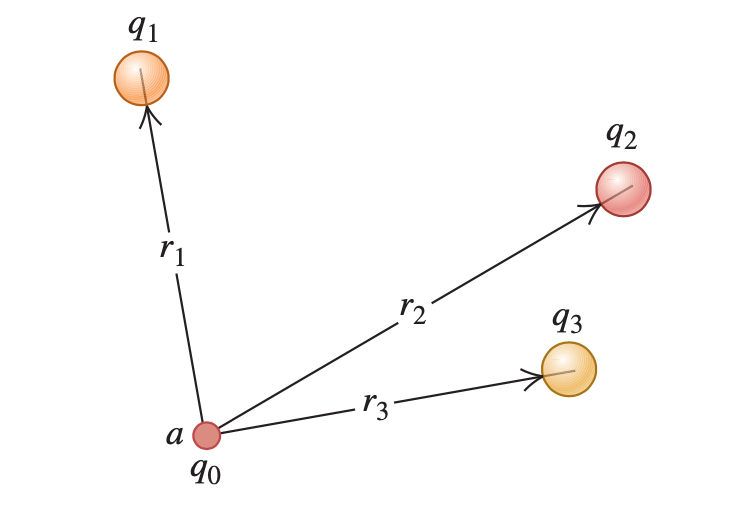
\includegraphics[scale=0.4]{fig/e_potencial_varias}
\label{fig:e_potencial_varias}
\end{figure}

Suponga que el campo eléctrico $\vec{E}$ en el que se desplaza la carga $q_0$ se debe a varias cargas puntuales $q_1, q_2, q_3$, . . . a distancias $r_1, r_2, r_3$, . . . de $q_0$. . El campo eléctrico total en cada punto es la \textit{suma vectorial} de los campos debidos a las cargas individuales, y el trabajo total realizado sobre $q_0$ durante cualquier desplazamiento es la suma de las contribuciones de las cargas individuales. De la ecuación \ref{23.9.e_potencial} se concluye que la energía potencial asociada con la carga de prueba $q_0$ en el punto a en la figura \ref{fig:e_potencial_varias} es la suma \textit{algebraica} (no la suma vectorial).

\begin{equation}\label{23.10}\marginnote{Carga puntual $q_0$ y conjunto de cargas $q_i$}
\boxed{U=\frac{q_0}{4\pi\epsilon_0}\left(\frac{q_1}{r_1}+\frac{q_2}{r_2}+\frac{q_3}{r_3}+\cdots \right)=\frac{q_0}{4\pi\epsilon_0}\sum_{i}\frac{q_i}{r_i}}
\end{equation}

El trabajo efectuado sobre la carga $q_0$ cuando se desplaza de $a$ a $b$ a lo largo de cualquier trayectoria es igual a la diferencia $U_a-U_b$ entre las energías potenciales cuando $q_0$ está en $a$ y en $b$.

Se puede representar \textit{cualquier} distribución de carga como un conjunto de cargas puntuales, por lo que la ecuación \ref{23.10} muestra que \textbf{para todo campo eléctrico debido a una distribución de carga estática, la fuerza ejercida por ese campo es conservativa.}

Las ecuaciones \ref{23.9.e_potencial} y \ref{23.10} definen que $U$ es igual a cero cuando todas las distancias $r_1, r_2, . . .$ son infinitas, es decir, cuando la carga de prueba $q_0$ está muy lejos de todas las cargas que producen el campo.

\subsubsection{Interpretación de la energía potencial eléctrica}
Definimos la energía potencial eléctrica en términos del trabajo realizado por el campo eléctrico sobre una partícula con carga que se mueve en el campo. Cuando una partícula se desplaza del punto $a$ al punto $b$, el trabajo que realiza sobre ella el campo eléctrico es $W_{a\to b}=U_a-U_b$. Por lo tanto, la diferencia de energía potencial $U_a-U_b$ es igual al \textit{trabajo que efectúa la fuerza eléctrica cuando la partícula se desplaza de $a$ a $b$}. Cuando $U_a$ es mayor que $U_b$ el campo realiza trabajo positivo sobre la partícula conforme “cae” de un punto de mayor energía potencial ($a$) a otro con menor energía potencial ($b$).

Un punto de vista alternativo pero equivalente es considerar cuánto trabajo se hubiera tenido que hacer para “subir” la partícula desde un punto $b$, en el que la energía potencial es $U_b$, hasta un punto $a$ en el que la energía potencial tiene un valor mayor $U_a$ (por ejemplo, al empujar dos cargas positivas para acercarlas). Para mover la partícula lentamente (de manera que no se le imparta ninguna energía cinética), es necesario ejercer una fuerza externa adicional $F_{ext}$ que es igual y opuesta a la fuerza del campo eléctrico y realiza un trabajo positivo. La diferencia de energía potencial $U_a-U_b$ se define entonces como el trabajo que debe efectuar una fuerza externa para desplazar la partícula lentamente desde $b$ hasta $a$ en contra de la fuerza eléctrica.

\section{Potencial eléctrico}
El \textbf{potencial} es \textit{la energía potencial por unidad de carga}. Se define el potencial $V$ en cualquier punto en el campo eléctrico como la energía potencial $U$ \textit{por unidad de carga} asociada con una carga de prueba $q_0$ en ese punto:

\begin{equation}\label{23.12}
V=\frac{U}{q_0} \quad\text{o bien, }\quad   U=q_0V
\end{equation}

La unidad del SI para el potencial es el \textbf{volt} (1 V):

\begin{equation*}
1\, \text{V}=1\, \text{J/C}
\end{equation*}

Dividiendo la ecuación \ref{23.2} entre $q_0$:

\begin{equation}\label{23.13}
\frac{W_{a\to b}}{q_0}=-\frac{\Delta U}{q_0}=-\left(\frac{U_b}{q_0}-\frac{U_a}{q_0}\right)=-(V_b-V_a)=V_a-V_b
\end{equation}

$V_a$ y $V_b$ se denominan el \textit{potencial en el punto a} y \textit{potencial en el punto b}, respectivamente. De este modo, el trabajo realizado por unidad de carga por la fuerza eléctrica cuando un cuerpo con carga se desplaza de $a$ a $b$ es igual al potencial en $a$ menos el potencial en $b$.

La diferencia $V_a-V_b$ se llama \textit{potencial de $a$ con respecto a $b$}; en ocasiones esa diferencia se abrevia como $V_{ab}=V_a-V_b$. En los circuitos eléctricos, a diferencia de potencial entre dos puntos con frecuencia se denomina \textbf{voltaje}. Así, la ecuación \ref{23.13} establece: \textbf{$V_{ab}$, el potencial de $a$ con respecto a $b$, es igual al trabajo realizado por la fuerza eléctrica cuando una UNIDAD de carga se desplaza de $a$ a $b$}. Otra interpretación válida tambien es \textbf{$V_{ab}$, el potencial de $a$ con respecto a $b$, es igual al trabajo que debe efectuarse para desplazar con lentitud una UNIDAD de carga de b a a contra la fuerza eléctrica}.

\subsection{Cálculo del potencial eléctrico}
Para encontrar el potencial $V$ debido a una sola carga puntual $q$, se divide la ecuación 	\ref{23.9.e_potencial} entre $q_0$:

\begin{equation}\label{23.14}\marginnote{Potencial debido a una carga puntual}
\boxed{V=\frac{U}{q_0}=\frac{1}{4\pi\epsilon_0}\frac{q}{r}}
\end{equation}

El potencial, como el campo eléctrico, es independiente de la carga de prueba $q_0$ que se utiliza para definirlo.

Para encontrar el potencial debido a un conjunto de cargas puntuales, se divide la ecuación \ref{23.10} entre $q_0$:

\begin{equation}\label{23.15}\marginnote{Potencial debido a un conjunto de cargas puntuales}
\boxed{V=\frac{U}{q_0}=\frac{1}{4\pi\epsilon_0}\sum_i\frac{q_i}{r_i}}
\end{equation}

Cuando se tiene una distribución continua de carga a lo largo de una línea, sobre una superficie o a través de un volumen, se divide la carga en elementos $dq$ y la suma en la ecuación \ref{23.15} se convierte en integral:

\begin{equation}\label{23.16}\marginnote{Potencial debido a un distribución contínua de carga}
\boxed{V=\frac{1}{4\pi\epsilon_0}\int\frac{dq}{r}}
\end{equation}

donde $r$ es la distancia que hay entre el elemento con carga $dq$ y el punto del campo donde se desea obtener $V$

\textbf{Observación}: El \textit{potencial} eléctrico en cierto punto es la energía potencial que estaría asociada a una carga \textit{unitaria} colocada en ese punto. Asimismo, hay que recordar que no tiene que haber una carga en un punto dado para que ahí exista un p tencial $V$.

\subsection{Obtención del potencial eléctrico a partir del campo eléctrico}
La fuerza $\vec{F}$ sobre una carga de prueba $q_0$ se escribe como $\vec{F}=q_0\vec{E}$ por lo que, según la ecuación \ref{23.1}, el trabajo realizado por la fuerza eléctrica conforme la carga de prueba se desplaza de $a$ a $b$ está dado por: 

\begin{equation*}
W_{a\to b}=\int_a^b\vec{F}\cdot d\vec{l}=\int_a^bq_0\vec{E\cdot d\vec{l}}
\end{equation*}

Si se divide entre $q_0$ y se compara el resultado con la ecuación \ref{23.13}, se encuentra que

\begin{equation}\label{23.17}\marginnote{Diferencial de potencial como integral de $\vec{E}$}
\boxed{V_a-V_b=\int_a^b\vec{E}\cdot d\vec{l}=\int_a^bE\cos\phi dl}
\end{equation}

El valor de $V_a-V_b$ es independiente de la trayectoria tomada de $a$ a $b$, del mismo modo en que el valor de $W_{a\to b}$ es independiente de la trayectoria. Para encontrar la ecuación \ref{23.17} hay que recordar que $\vec{E}$ es la fuerza eléctrica por unidad de carga sobre una carga de prueba.

La regla general, válida para \textit{cualquier} campo eléctrico, es la siguiente: desplazarse \textit{en} la dirección de $\vec{E}$ significa hacerlo en la dirección de $V$ \textit{decreciente}, y desplazarse \textit{contra de} la dirección de $\vec{E}$ signifca moverse en la dirección de $\vec{E}$ \textit{creciente}.

Observe que la ecuación \ref{23.17} se puede escribir como 

\begin{equation}\label{23.18}
V_a-V_v=-\int_b^{a}\vec{E}\cdot d\vec{l}
\end{equation}

La ecuación \ref{23.18} se puede interpretar de la siguiente manera: Para mover una unidad de carga lentamente en contra de la fuerza eléctrica, se debe aplicar una fuerza externa por unidad de carga igual a $-\vec{E}$, igual y opuesta a la fuerza eléctrica por unidad de carga $\vec{E}$.

\section{Cálculo del potencial eléctrico}
Cuando se calcula el potencial debido a una distribución de carga, por lo general se sigue una de dos rutas posibles. Si se conoce la distribución de carga se emplea la ecuación \ref{23.15} o la \ref{23.16}. O si se conoce el modo en que el campo eléctrico depende de la posición, se usa la ecuación \ref{23.17} estableciendo que el potencial es igual a cero en algún lugar conveniente.

\section{Superficies equipotenciales}
Una \textbf{superficie equipotencial} es una superficie tridimensional sobre la que el \textit{potencial eléctrico} $V$ es el mismo en todos los puntos. Si una carga de prueba $q_0$ se desplaza de un punto a otro sobre tal superficie, la energía potencial \textit{eléctrica} $q_0V$ permanece constante. Ningún punto puede estar en dos potenciales diferentes, por lo que las superficies equipotenciales para distintos potenciales nunca se tocan o intersecan.

\subsection{Superficies equipotenciales y líneas de campo}
Como la energía potencial no cambia a medida que una carga de prueba se traslada sobre una superficie equipotencial, el campo eléctrico no realiza trabajo sobre esa carga. De ello se deriva que $\vec{E}$ debe ser perpendicular a la superficie en cada punto, de manera que la fuerza eléctrica $q_0\vec{E}$ siempre es perpendicular al desplazamiento de una carga que se mueva sobre la superficie. \textbf{Las líneas de campo y las superficies equipotenciales siempre son perpendiculares entre sí}.

\textbf{Obervación}: En una superficie equipotencial dada, el potencial $V$ tiene el mismo valor en todos los puntos. Sin embargo, en general la magnitud del campo eléctrico $\vec{E}$ \textit{no} es la misma en todos los puntos sobre una superficie equipotencial.

\subsection{Equipotenciales y conductores}
\textbf{Cuando todas las cargas están en reposo, la superficie de un conductor siempre es una superficie equipotencial}. Como el campo eléctrico $\vec{E}$ siempre es perpendicular a una superficie equipotencial, el enunciado se puede demostrar si se prueba que \textbf{cuando todas las cargas están en reposo, el campo eléctrico justo afuera de un conductor debe ser perpendicular a la superficie en cada punto}. Se sabe que $\vec{E}=0$ en todos los lugares del interior del conductor; de otro modo, las cargas se moverían. $\vec{E}$ es perpendicular a la superficie en cada punto.

\section{Gradiente de potencial}
En la ecuación \ref{23.17}, $V_a-V_b$ es el potencial de $a$ con respecto de $b$, es decir, el cambio de potencial encontrado en un despalzamiento de $b$ a $a$. Esto es 

\begin{equation*}
V_a-V_b=\int_b^adV=-\int	_a^bdV
\end{equation*}

donde $dV$ es el cambio infinitesimal del potencial que acompaña un elemento infinitesimal $d\vec{l}$ de la trayectoria de $b$ a $a$. Comparando con la ecuación \ref{23.17} se tiene

\begin{equation*}
-\int_a^bdV=\int_a^b\vec{E}\cdot d\vec{l}
\end{equation*}

Estas dos integrales deben ser iguales para \textit{cualquier} par de límites $a$ y $b$, y para que esto se cumpla los \textit{integrados} deben ser iguales. Por lo tanto, para cualquier desplazamiento infinitesimal $$-dV=\vec{E}\cdot d\vec{l}$$

Las componentes de $\vec{E}$ se relacionan con las derivadas correspondientes de $V$ de la siguiente forma

\begin{equation}\label{23.19}\marginnote{Componentes de $\vec{E}$ en términos de $V$}
\boxed{E_x=-\frac{\partial V}{\partial x} \quad E_y=-\frac{\partial V}{\partial y} \quad E_z=-\frac{\partial V}{\partial z}}
\end{equation}

En términos de vectores unitarios, $\vec{E}$ se escribe como

\begin{equation}\label{23.20}\marginnote{$\vec{E}$ en términos de $V$}
\boxed{\vec{E}=-\left(\hat{i}\frac{\partial V}{\partial x}+\hat{j}\frac{\partial V}{\partial y}+\hat{k}\frac{\partial V}{\partial z}\right)}
\end{equation}

O en forma equivalente

\begin{equation}\label{23.22}
\vec{E}=-\vec{\nabla} V
\end{equation}














































\chapter{Fuentes de campo magnético}
\section{Campo de una carga en movimiento}
Comenzaremos con lo fundamental: el campo magnético de una sola carga puntual $q$ que se mueve con velocidad constante $\vec{v}$. Los experimentos demuestran que la magnitud de $\vec{B}$ es proporcional a $|q|$ y a $1/r^2$, pero su dirección \textit{no} es a lo largo de de la línea que va desde el punto de fuente al punto de campo. En vez de ello, $\vec{B}$ es perpendicular al plano que contiene esta línea y al vector velocidad, de la partícula, $\vec{v}$. Además, la magnitud $\vec{B}$ del campo también es proporcional a la rapidez $\vec{v}$ de la partícula y al seno del ángulo $\phi$. Así, la magnitud del campo magnético en el punto $P$ está dada por
\begin{equation}\label{28.1}
B=\frac{\mu_0}{4\pi}\frac{|q|v\sin\phi}{r^2}
\end{equation}
donde $\mu_0/4\pi$ es una constante de proporcionalidad.
En forma vectorial
\begin{equation}\marginnote{C. magnético de una carga puntual con velocidad constante}
\boxed{\vec{B}=\frac{\mu_0}{4\pi}\frac{q\vec{v}\times\hat{r}}{r^2}}
\end{equation}
\textbf{Nota}: Las partículas con carga que constituyen una corriente en un alambre aceleran en los puntos en que éste se dobla y la dirección de $\vec{v}$ cambia. Pero como la magnitud $v_d$ de la velocidad de deriva en un conductor por lo general es muy pequeña, la aceleración $v_d^2/r$ también lo es, por lo que pueden ignorarse los efectos de la aceleración.

La unidad en el SI de $B$ es un \textbf{tesla} [1T].

En unidades del SI, el valor numérico de $\mu_0$ es exactamente $4\pi\times 10^{-7}$
\section{Campo magnético de un elemento de corriente}
\textbf{Principio de superposición de campos magnéticos}:  El campo magnético total generado por varias cargas en movimiento es la suma vectorial de los campos generados por las cargas individuales.

\textit{Cálculo del campo magnético ocasionado por un segmento corto $d\vec{l}$ de un conductor que transporta corriente}:

El volumen del segmento es $A dl$, donde $A$ es el área de la sección transversal del conductor. Si hay $n$ partículas con carga en movimiento por unidad de volumen, cada una con una carga $q$, la carga total $dQ$ que se mueve en el segmento es $$dQ=nqAdl$$ Las cargas en movimiento en este segmento son equivalentes a una sola carga $dQ$
que viaja con una velocidad igual a la velocidad de \textit{deriva} $\vec{v}_d$. (Los campos magnéticos debidos a los movimientos al azar de las cargas, en promedio, se cancelarán en cada punto.) De ec. \ref{28.1}, la magnitud del campo resultante $d\vec{B}$ en cualquier punto $P$ es
\begin{equation}\label{28.5}
dB=\frac{\mu_0}{4\pi}\frac{|dQ|v_d\sin\phi}{r^2}=\frac{\mu_0}{4\pi}\frac{n|q|v_dAdl\sin\phi}{r^2}=\frac{\mu_o}{4\pi}\frac{Idl\sin\phi}{r^2}
\end{equation} 
porque de ec (25.2), $n|q|v_dA$ es igual a la corriente $I$ en el elemento.

En su forma vectorial
\begin{equation}\label{28.6}\marginnote{C. magnético de un elemento de corriente}
\boxed{d\vec{B}=\frac{\mu_0}{4\pi}\frac{Id\vec{l}\times\hat{r}}{r^2}}
\end{equation}
donde $d\vec{l}$ es un vector con longitus $dl$, en la misma dirección que la corriente del coductor.
 
Las ecuaciónes \ref{28.5} y \ref{28.6} constituyen la \textbf{ley de Biot y Savat}. Esta ley se utiliza para encontrar el campo magnético total $B$ debido a la corriente en un circuito completo en cualquier punto en el espacio.
\section{Campo magnético de un conductor que transporta corriente}
\begin{figure}[h]
\centering
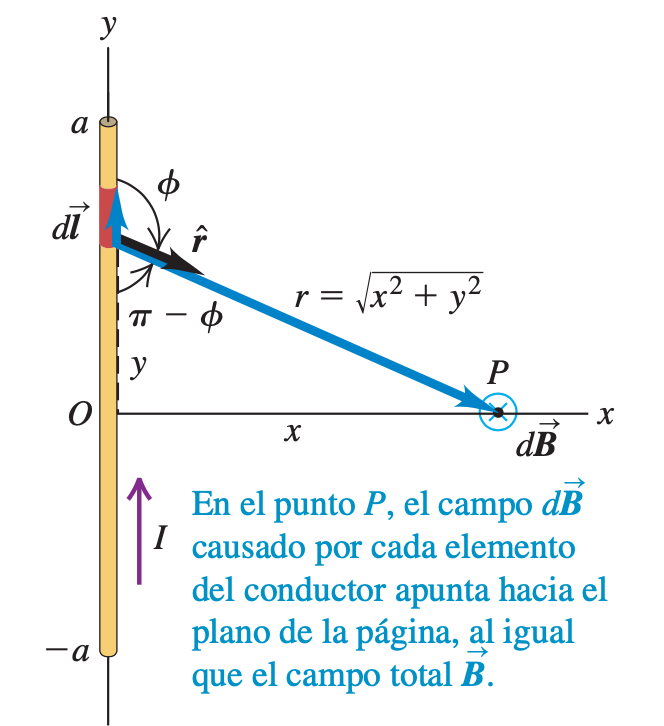
\includegraphics[scale=0.6]{fig/image1}
\caption{Campo magnético producido por un conductor recto portador de corriente de longitud infinita.}
\label{fig:28.5}
\end{figure}
Usando la ley de Biot y Savat, ecuación \ref{28.6}, y haciendo los cálculos correspondientes, se tiene que $B$ debe tener la misma magnitud en todos los puntos de un círculo con centro en el conductor y que yace en un plano perpendicular a él, y la dirección de $B$ debe ser tangente a todo ese círculo. Así, 
\begin{equation}\label{28.9}\marginnote{C. magnético cerca de un conductor largo y recto portador de corriente}
\boxed{\vec{B}=\frac{\mu_0I}{2\pi r}\hat{\phi}}
\end{equation}
\textbf{Observaciones:}
\begin{enumerate}
\item Las líneas de campo magnético circundan la corriente que actúa como su fuente.
\item Las líneas del campo magnético forman espiras cerradas y \textit{nunca} tienen extremos, sin importar la forma del conductor portador de corriente que genera el campo. Ésta es una consecuencia de la ley de Gauss para el magnetismo, que plantea que el flujo magnético total a través de cualquier superficie cerrada siem- pre es igual a cero:
\begin{equation}\label{28.10}
\oint\vec{B}\cdot d\vec{A}=0
\end{equation}
Esto implica que no hay cargas magnéticas aisladas ni monopolos magnéticos. \textbf{Cualquier línea de campo magnético que entre a una superficie cerrada debe salir de ella}.
\end{enumerate}
\section{Fuerza entre alambres paralelos}
\begin{figure}[h]\label{fig2}
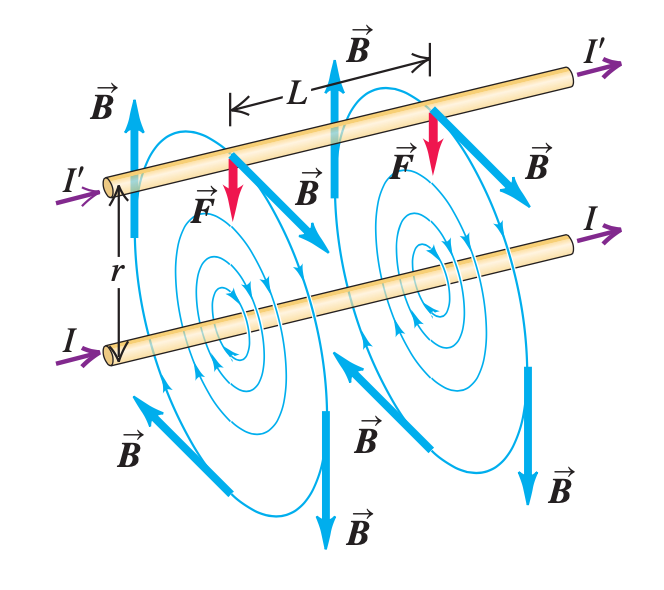
\includegraphics[scale=0.6]{fig/image2}
\centering
\end{figure}
De acuerdo con la ecuación \ref{28.9}, el conductor inferior produce un campo $\vec{B}$ que, en la posición del conductor de arriba, tiene una magnitud $$B=\frac{\mu_0I}{2\pi r}$$ De ecuación (27.19) la fuerza que ejerce este campo sobre una longitud $L$ del conductor superior es $\vec{F}=I' \vec{L}\times\vec{B}$,  donde el vector $\vec{L}$ está en dirección de la corriente $I'$ y tiene magnitud $L$. Como $\vec{B}$ es perpendicular a la longitud del conductor y, por lo tanto, a $\vec{L}$, la magnitud de esta fuerza es $$F=I'LB=\frac{\mu_oII'L}{2\pi r}$$ Luego, la \textit{fuerza por unidad de longitud}, $F/L$ está dada por
\begin{equation}\label{28.11}\marginnote{Magnitud de la fza. entre dos coductores largos, paralelos y portadores de
corriente}
\boxed{\frac{F}{L}=\frac{\mu_0II'}{2\pi r}}
\end{equation}
La aplicación de la regla de la mano derecha a $\vec{F}=I'\vec{L}\times\vec{B}$ indica que la fuerza sobre el conductor de arriba está dirigida hacia abajo.

\textbf{Observación}:
\begin{enumerate}
\item Dos conductores paralelos que transportan corrientes en el mismo sentido se atraen uno al otro.
\item Dos conductores paralelos que transportan corrientes en sentido opuestos se repelen entre sí.
\end{enumerate}
\section{Campo magnético de una espira circular de corriente}
\begin{figure}[h]\label{fig3}
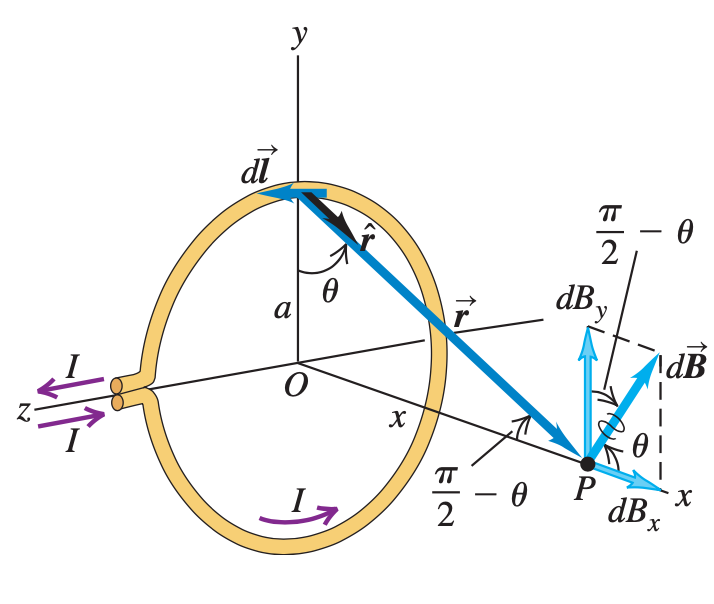
\includegraphics[scale=0.6]{fig/image3}
\centering
\end{figure}
Para encontrar el campo magnético en el punto $P$ sobre el eje de la espira, se usa la ley de Biot y Savart, ecuación \ref{28.5} o \ref{28.6}. De la figura \ref{fig3}, $d\vec{l}$ y $\vec{r}$ son perpendiculares, y la dirección del campo $d\vec{B}$ generado por este elemento $d\vec{l}$ en particular yace sobre el plano $xy$. La magnitud $dB$ del campo debido al elemento $d\vec{l}$ es
\begin{equation}\label{28.15}
\boxed{B_x=\frac{\mu_0Ia^2}{2(x^2+a^2)^{3/2}}}
\end{equation}
Si se cierran los dedos de la mano derecha alrededor de la espira en la dirección de la corriente, el pulgar derecho apunta en la dirección del campo.
\subsection{Campo magnético sobre el eje de una bobina}
Ahora suponga que en vez de una sola espira en la figura \ref{fig3}, se tiene una bobina que consiste en N espiras. Cada espira contribuye por igual al campo, y el total es N veces el campo producido por una sola espira:
\begin{equation}\label{28.16}
B_x=\frac{\mu_0NIa^2}{2(x^2+a^2)^{3/2}}
\end{equation}
En el centro de $N$ espiras circulares la magnitud del campo magnético vale
\begin{equation}\label{28.17}
\boxed{B_x=\frac{\mu_0Ia^2}{2a}}
\end{equation}
Conforme se avanza a lo largo del eje, la magnitud del campo disminuye.
\textbf{Observación}: Las ecuaciones \ref{28.15} y \ref{28.16} son válidas sólo sobre el \textit{eje} de una espira o bobina. No sobre otros puntos.


\section{Ley de Ampere}
\begin{equation}\label{28.20.ampere}\marginnote{Ley de Ampere}\footnote{Sólo válida si las corrientes son estables y si no están presentes materiales magnéticos o campos eléctricos que varíen con el tiempo.}
\boxed{\oint\vec{B}\cdot d\vec{l}=\mu_0I_{enc}}
\end{equation}
Hay una regla simple para determinar el signo de la corriente; Doble los dedos de su mano derecha alrededor de la trayectoria de integración en la dirección de esta última, es decir, la dirección que usa para evaluar $\oint\vec{B}\cdot d\vec{l}$. En esas condiciones, su pulgar derecho indica la dirección de la corriente positiva. Las corrientes que pasan a través de la trayectoria de integración en esta dirección son positivas; aquéllas en dirección opuesta son negativas. La ecuación \ref{28.20.ampere} de hecho es válida para conductores y trayectorias de \textbf{cualquier} forma.

\textbf{Observación}: Si $\oint\vec{B}\cdot d\vec{l}=0$, no necesariamente significa que $\vec{B}=0$
\subsection{Campo de un soleoide}
\begin{figure}[h]
\centering
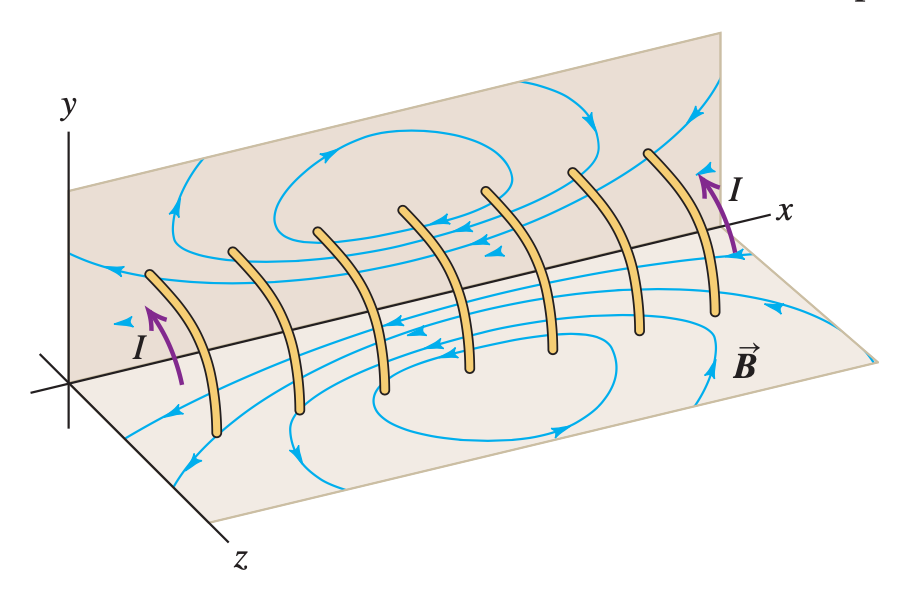
\includegraphics[scale=0.4]{fig/solenoide1}
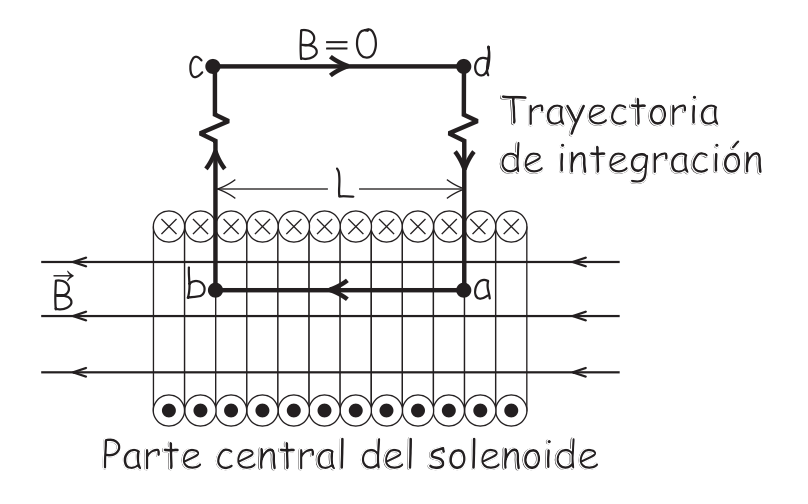
\includegraphics[scale=0.4]{fig/solenoide2}
\end{figure}
Aplicando la ley de Ampere, ecuación \ref{28.20.ampere}, junto con la trayectoria mostrada, se tiene que 
\begin{equation}
B=\mu_0nI
\end{equation}
teniendo en cuenta que $I_{enc}=nLI$.
\subsection{Campo de un solenoide toroidal(toroide)}
\begin{figure}[t]
\centering
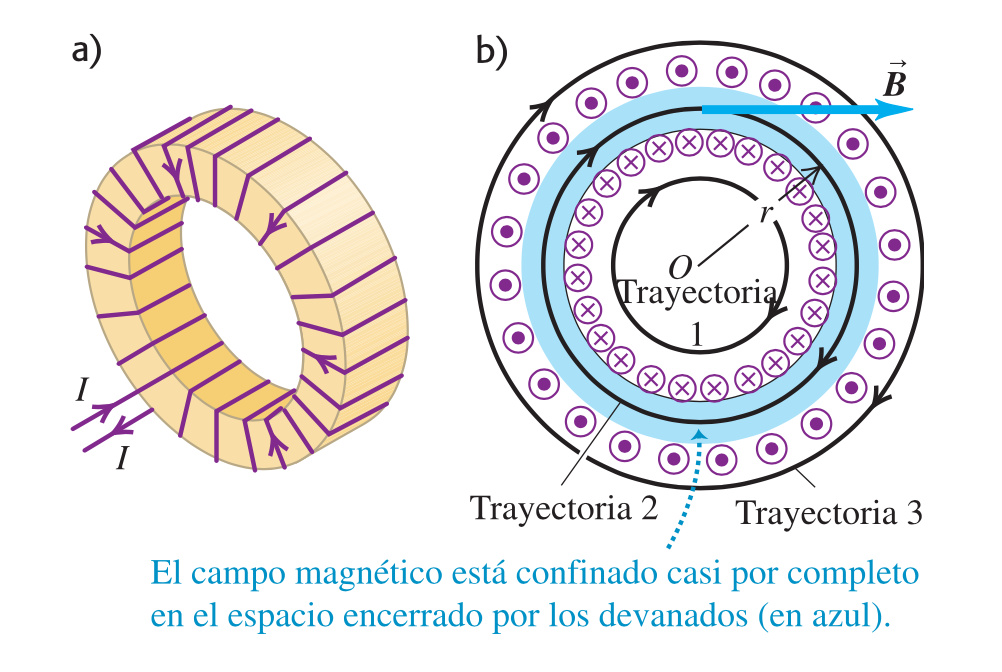
\includegraphics[scale=0.5]{fig/toroide}
\end{figure}
Considerando la trayectoria de integración 1. No hay corriente encerrada, luego $\vec{B}=0$ en cualquier punto de esta trayectoria.

Considernado la trayectoria de integración 3. Cada espira pasa dos veces a través del área limitada por esta trayectoria, llevando corrientes iguales en sentidos opuestos. Luego $I_{enc}=0\rightarrow \vec{B}=0$ en todos los puntos de esta trayectoria.

Considerando la trayectoria 2, un círculo con radio $r$. Se espera que el campo $\vec{B}$ sea tangente a la trayectoria. Por tanto, $\oint\vec{B}\cdot d\vec{l}=2\pi rB$. Despejando $B$
\begin{equation}\label{28.24.toroide}
B=\frac{\mu_0NI}{2\pi r}
\end{equation}
%\end{document}

\chapter{Inducción electromagnética}
La fuente de fem no es una batería, sino una estación generadora de electricidad.
La inducción electromagnética nos dice que un campo magnético que varía en el tiempo actúa como fuente de campo eléctrico.
También, un campo eléctrico que varía con el tiempo actúa como fuente de un campo magnético

\section{Ley de Faraday}
El flujo magnético total $\Phi_B$ a través de un área finita es la integral de esta expresión sobre el área:
\begin{equation}\label{29.1}
\Phi_B=\int\vec{B}\cdot d\vec{A}=\int B\, dA\cos\phi
\end{equation}
En el caso de que $\vec{B}$ sea uniforme sobre un área plana $\vec{A}$, entonces
\begin{equation}\label{29.2}
\Phi_B=\vec{B}\cdot \vec{A}=BA\cos\phi
\end{equation}
La \textbf{Ley de Faraday de la inducción} establece lo siguiente:
\textit{La fem inducida en una espira cerrada es igual al negativo de la tasa de cambio del flujo magnético a través de la espira con respecto al tiempo}.
 
En símbolos
\begin{equation}\marginnote{Ley de Faraday}\label{29.3.faraday}
\boxed{\varepsilon=-\frac{d\Phi_B}{dt}}
\end{equation}
\textbf{Obervación}: Las fem inducidas son ocasionadas por \textbf{cambios de flujo}.

Si se tiene una bobina con $N$ espiras idénticas y si el flujo varía a la misma tasa a través de cada espira, la fem total en la bobina es
\begin{equation}\label{29.4.Nfaraday}
\boxed{\varepsilon=-N\frac{d\Phi_B}{dt}}
\end{equation}
La \textbf{Ley de Lenz} establece que, \textit{la dirección de cualquier efecto de la inducción magnética es la que se opone a la causa del efecto.}
\section{Fuerza electromotriz de movimiento}
\begin{figure}[h]
\centering
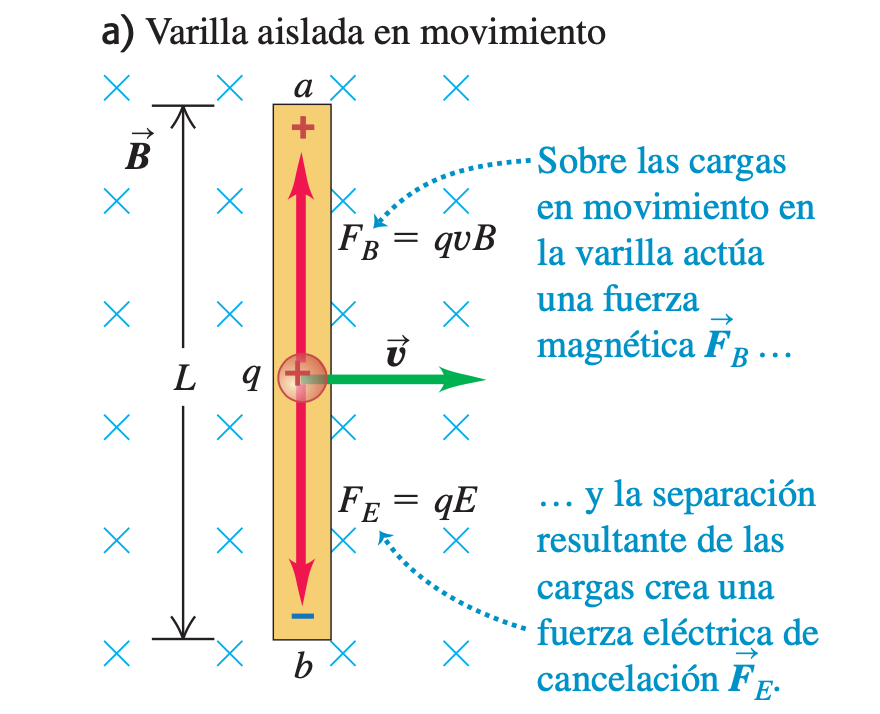
\includegraphics[scale=0.5]{fig/varilla}
\end{figure}
Una partícula cargada $q$ (	que suponemos positiva) en la varilla experimenta una fuerza magnética $\vec{F}=q\vec{v}\times\vec{B}$ con magnitud $F=|q|vB$. Esta fuerza magnética hace que las cargas libres en la varilla se muevan, lo que crea un exceso de carga positiva en el extremo superior $a$ y de carga negativa en el extremo inferior $b$.
Esto, a la vez, crea un campo eléctrico $\vec{E}$ en el interior de la varilla, en el sentido que va de $a$ hacia $b$ (opuesto al campo magnético). Llega un momento en el que $\vec{E}$ es lo suficientemente grande como para que la fuerza eléctrica ($qE$) cancele exáctamente a la magnética. De esta manera, $qE=qvB$, y las cargas están en equilibrio. Luego, se tiene que
\begin{equation}\label{29.5}
V_{ab}=V_a-V_b=EL=qBL
\end{equation}
con el punto $a$ a un potencial mayor que $b$.
\textbf{Continua...}
\subsection{Fem de movimiento: Forma general}
Podemos generalizar el concepto de fem de movimiento para un conductor de cualquier forma que se mueva en un campo magnético, uniforme o no (suponiendo que el campo magnético en cada punto no varía con el tiempo). Para cualquier fem cerrada, la fem total es
\begin{equation}\label{29.7}
\varepsilon=\oint (\vec{v}\times\vec{B})\cdot d\vec{l}
\end{equation}
Cuando se tienen conductores fijos en campos magnéticos cambiantes, no es posible utilizar la ecuación \ref{29.7}. En tal caso utilizar la ley de Faraday, ecuación \ref{29.3.faraday}.


\section{Campo eléctricos inducidos}
Una fem inducida también se presenta cuando hay un flujo cambiante a través de un conductor fijo.

\begin{figure}[h]\label{fig:galvanometro}
\centering
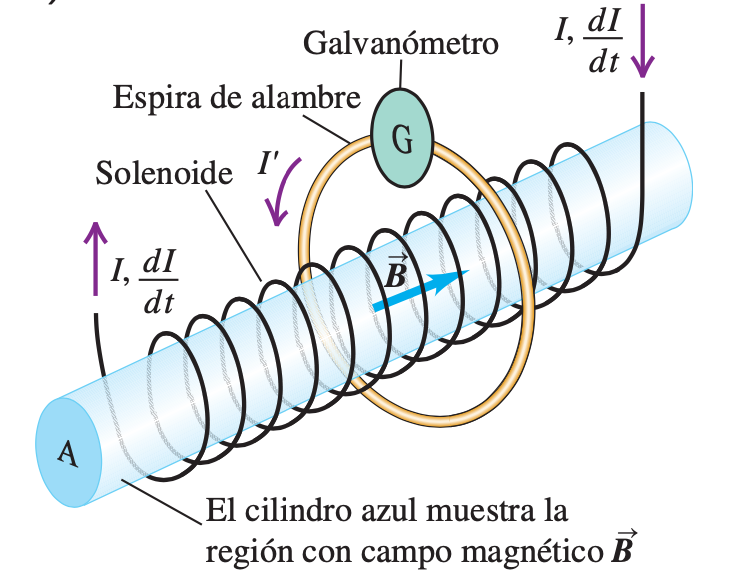
\includegraphics[scale=0.5]{fig/galvanometro}
\caption{El devanado de un solenoide largo lleva una corriente que se incrementa a una tasa $dI>dt$. El flujo magnético en el solenoide aumenta a una tasa $d\Phi_B/dt$, y este flujo cambiante pasa a través de una espira de alambre. En la espira se induce una fem $\varepsilon= -d\Phi_B/dt$, la cual induce una corriente $I'$ que se mide con el galvanómetro G}
\end{figure}

Consideremos la situacion que se ilustra en la figura \ref{fig:galvanometro}. Un solenoide largo y delgado, con área de sección transversal $A$ y $n$ espiras por unidad de
longitud, está rodeado en su centro por una espira conductora circular. El galvanómetro G mide la corriente en la espira. Una corriente $I$ en el devanado del solenoide establece un campo magnético $\vec{B}$ a lo largo de su eje, como se indica, con magnitud $B=\mu_0nI$, donde $n$ es el número de espiras por unidad de longitud. El flujo magnético a traves de la espira es $$\Phi_B=BA=\mu_0nIA$$ Cuando la corriente $I$ cambia con el tiempo se tiene, según la ley de Faraday

\begin{equation}\label{29.8}
\varepsilon=-\frac{d\Phi_B}{dt}=-\mu_0nA\frac{dI}{dt}
\end{equation}

Si la resistencia total de la espira es $R$, la corriente inducida en la espira es $I'=\varepsilon/R$. ¿Qué fuerza hace que las cargas se muevan alrededor de la espira? No puede ser una fuerza magnética porque el conductor no se está moviendo en un campo magnético, y en realidad ni siquiera está en un campo magnético. Se debe a un \textbf{campo magnético inducido} en el conductor \textit{causado por el flujo magnético cambiante}. Este campo eléctrico en la espira \textbf{no es conservativo}, porque la integral de línea de $\vec{E}$ a lo largo de la trayectoria cerrada no es igual a cero. En vez de ello, esta integral de línea, que representa el trabajo realizado por el campo inducido $\vec{E}$ por unidad de carga, es igual a la fem inducida $\varepsilon$:

\begin{equation}\label{29.9}
\oint\vec{E}\cdot d\vec{l}=\varepsilon
\end{equation}

Que según la ley de Faraday

\begin{equation}\label{29.10}\marginnote{Trayectoria de integración constante}
\boxed{\oint\vec{E}\cdot d\vec{l}=-\frac{d\Phi_B}{dt}}
\end{equation}

La forma de la ley de Faraday dada en la ecuación \ref{29.10}, sólo es válida si la trayectoria alrededor de la cual se integra es \textbf{constante}.

Un campo de esta clase recibe el nombre de \textbf{campo no electrostático}. Este campo, a pesar de no ser conservativo, ejerce una fuerza $\vec{F}=q\vec{E}$ sobre una carga $q$. De esta manera, un campo magnético actúa como fuente de campo eléctrico de una clase que \textit{no podemos} producir con ninguna distribución de carga estática.

\section{Corriente de desplazamiento y ecuaciones de Maxwell}
De igual manera que un campo magnético que varía da lugar a un campo eléctrico inducido, un campo eléctrico variable, da lugar a un campo magnético.

\subsubsection{Generalización de la ley de Ampere}
Recordando la ley de Ampere, $$\oint\vec{B}\cdot d\vec{l}=\mu_0I_{enc}$$ Esta ley, expresada de esta manera está \textit{incompleta}.
\textbf{continua...}







%\end{document}

\chapter{Inductancia}
\section{Inductancia mutua}

\begin{figure}[h]
\centering
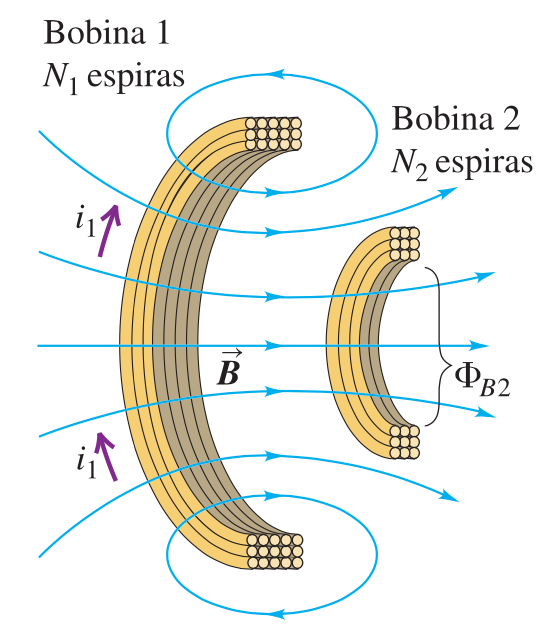
\includegraphics[scale=0.3]{fig/bobinas}
\caption{\textbf{Inductancia mutua}, si la corriente en la bobina 1 está cambiando, el flujo cambiante a través de la bobina 2 indice una fem en esta última}
\label{fig:bobinas}
\end{figure}
Interacción magnética entre dos alambres que trasnportan corrientes \textit{estables}; la corriente de uno de los alambres genera un campo magnético que ejerce una fuerza sobre la corriente entre el otro alambre. Cuando hay una corriente \textit{variable} en uno de los circuitos, surge una interacción adicional. Consideremos la situación de la figura
\ref{fig:bobinas}

Una corriente que circula por la bobina 1 produce un campo magnético $\vec{B}$ y, por lo tanto, un flujo magnético a través de la bobina 2. Si la corriente en la bobina 1 cambia, el flujo a través de la bobina 2 también cambia; de acuerdo con la ley de Faraday, esto induce una fem en la bobina 2. De este modo, un cambio en la corriente de un circuito puede inducir otra corriente en un segundo circuito.
Una corriente $i_1$\footnote{Denotamos con $i$ a una corriente variable en el tiempo } establece un campo magnético (indicado por las líneas de color azul), y algunas de estas líneas de campo pasan a través de la bobina 2. Denotaremos con $\Phi_{B2}$ el flujo magnético a través de \textit{cada} espira de la bobina 2, causado por la corriente $i_1$ en la bobina 1. (Si el flujo es diferente a través de las distintas espiras de la bobina, entonces $\Phi_{B2}$ denota el flujo  \textit{medio}). El campo magnético es proporcional a $i_1$, de manera que $\Phi_{B2}$ también es proporcional a $i_1$. \textbf{Cuando $i_1$ cambia, $\Phi_{B2}$ cambia; este flujo cambiante induce una fem $\varepsilon_2$ en la bobina 2}, dada por
\begin{equation}\label{fem}
\varepsilon_2=-N_2\frac{d\Phi_{B2}}{dt}
\end{equation}
Podríamos representar la proporcionalidad entre $\Phi_{B2}$ e $i_1$ en la forma $\Phi_{B2}$ = (constante) $i_1$, pero, en vez de ello, es más conveniente incluir el número de espiras $N_2$ en la relación. Al introducir una constante de proporcionalidad $M_{21}$, llamada \textbf{inductancia mutua} de las dos bobinas, escribimos
\begin{equation}\label{30.2}
N_2\Phi_{B2}=M_{21}i_1
\end{equation}
donde $\Phi_{B2}$ es el flujo a través de una sola espira de la bobina 2. De ahí que,
\begin{equation}
N_2\frac{d\Phi_{B2}}{dt}=M_{21}\frac{di_1}{dt}
\end{equation}
y la ecuación \ref{fem} se rescribe como
\begin{equation}
\varepsilon_2=-M_2\frac{di_1}{dt}
\end{equation}
Es decir, un cambio en la corriente $i_1$ en la bobina 1 induce una fem en la bobina 2, que es directamente proporcional a la tasa de cambio de $i_1$.

También se podría escribir la definición de la inductancia mutua, ecuación \ref{30.2}, como
\begin{equation}
M_{21}=\frac{N_2\Phi_{B2}}{i_1}
\end{equation}
\textbf{Si las bobinas están en el vacío}, el flujo $\Phi_{B2}$ a través de cada espira de la bobina 2 es directamente proporcional a la corriente $i_1$. Entonces, la inductancia mutua $M_{21}$ es una constante que sólo depende de la geometría de las dos bobinas.
Podría volverse a hacer el análisis para el caso opuesto, en el que una corriente cambiante $i_2$ en la bobina 2 causa un flujo cambiante $\Phi_{B}2$ y una fem $\varepsilon_1$ en la bobina 1. Se encuentra que, \textbf{$M_{12}$ siempre es igual a $M_{21}$, aun cuando las dos bobinas no sean simétricas}. A este valor común $M$ lo llamamos simplemente \textbf{inductancia mutua}. Por tanto, tenemos:
\begin{equation}\marginnote{Fem mutuamente inducidas}
\boxed{\varepsilon_2=-M\frac{di_1}{dt}\quad\mathrm{y}\quad \varepsilon_1=-M\frac{di_2}{dt}\quad}
\end{equation}
donde la inductancia mutua $M$ es
\begin{equation}\marginnote{Inductancia mutua}
\boxed{M=\frac{N_2\Phi_{B2}}{i_1}=\frac{N_1\Phi_{B1}}{i_2}}
\end{equation}
\textbf{Obs: Sólo una corriente variable en el tiempo induce una fem}.

La unidad del SI para la inductancia mutua se llama \textbf{henry} [$H$]
\section{Autoinductancia a inductores}
\begin{figure}[h]\label{fig:autoinductancia}
\centering
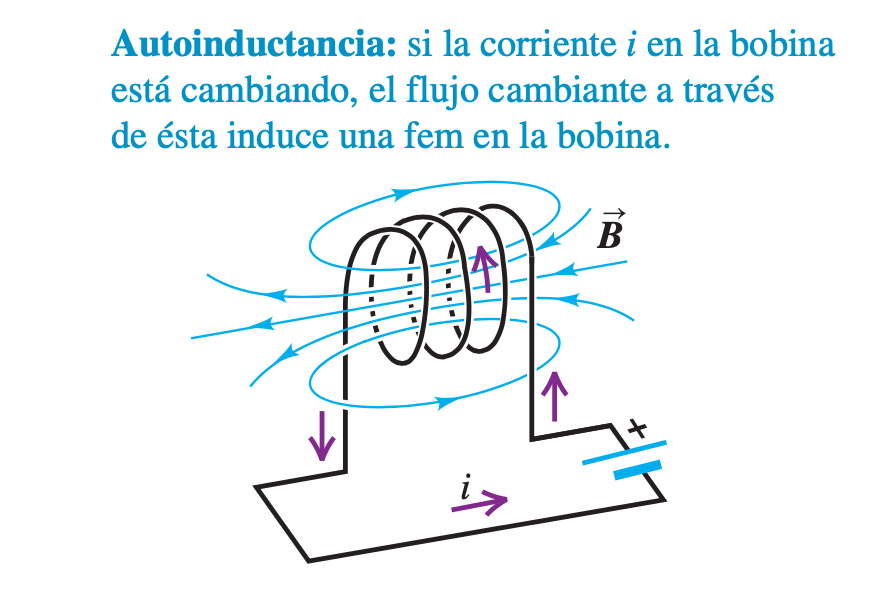
\includegraphics[scale=0.4]{fig/autoinductancia}
\caption{La corriente $i$ en el circuito crea un campo magnético $\vec{B}$ en la bobina y, por lo tanto, un flujo a través de ésta.}
\end{figure}

Consideremos un solo circuito aislado. Cuando en el circuito está presente una corriente, se establece un campo magnético que crea un flujo magnético a través del mismo circuito; este flujo cambia cuando la corriente cambia. Así, cualquier circuito que conduzca una corriente variable tiene una fem inducida en él por la variación en su propio campo magnético. Esa clase de fem se denomina \textbf{fem autoinducida}. Según la ley de Lenz, una fem autoinducida siempre se opone al cambio en la corriente que causó la fem, y de ese modo hace más difícil que haya variaciones en la corriente. El efecto se intensifica considerablemente si el circuito incluye una bobina con $N$ espiras de alambre. Como resultado de la corriente $i$, hay un flujo magnético medio $\Phi_B$ a través de cada vuelta de la bobina, figura \ref{fig:autoinductancia}.

Definimos la \textbf{autoinductancia} como
\begin{equation}\label{30.6.autoinductancia}\marginnote{Autoinductancia}
\boxed{L=\frac{N\Phi_B}{i}}
\end{equation}
Si la corriente $i$ en el circuito cambia, también lo hace el flujo $\Phi_B$. De ecuación \ref{30.6.autoinductancia} $$N\frac{d\Phi_B}{dt}=L\frac{di}{dt}$$ Utilizando la ley de Faraday, ecuación \ref{29.4.Nfaraday}, la fem autoinducida es
\begin{equation}\label{30.7}\marginnote{Fem autoinducida}
\boxed{\varepsilon=-L\frac{di}{dt}}
\end{equation}

\subsection{Los inductores como elementos de un circuito}
Un elemento de circuito diseñado para tener una inductancia particular se llama \textbf{inductor, o bobina de autoinducción}. Su finalidad es oponerse a cualquier variación en la corriente a través del circuito. Un inductor en un circuito de corriente directa ayuda a mantener una corriente estable a pesar de las fluctuaciones en la fem aplicada; en un circuito de corriente alterna, un inductor tiende a suprimir las variaciones de la corriente que ocurran más rápido de lo deseado.

Al utilizar la ley de Kirchhoff a traves de una malla conductora se suman sus diferencias de potencial y se igualan a cero porque el campo eléctrico producido por las cargas distribuidas es \textit{conservativo} ($\vec{E_c}$). El campo eléctrico inducido magnéticamente dentro de las bobinas del inductor \textbf{no es conservativo} ($\vec{E_n}$).


\begin{figure}[h]\label{fig30.5.circuito}
\centering
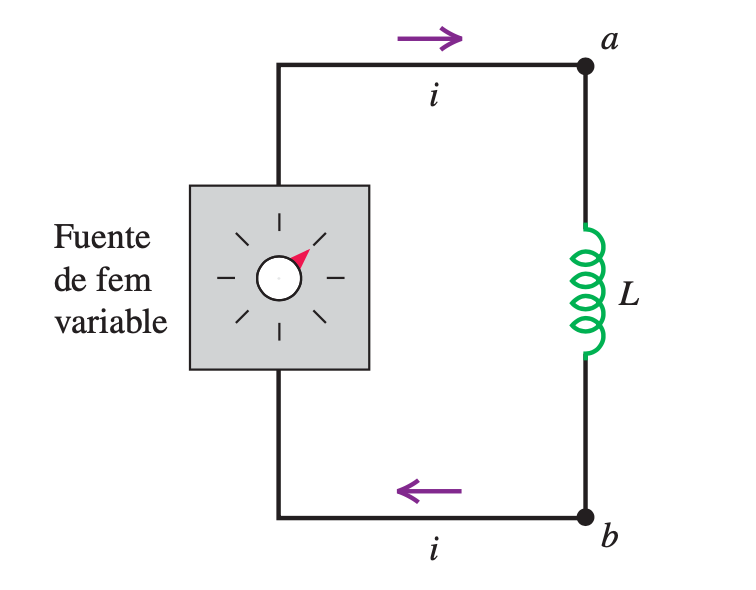
\includegraphics[scale=0.4]{fig/circuito}
\caption{Circuito que contiene una fuente de fem y un inductor. La fuente es variable, por lo que la corriente $i$ y su tasa de cambio $di>dt$ pueden variarse.}
\end{figure}

Consideremos el circuito de la figura \ref{fig30.5.circuito}. De acuerdo con la ley de Faraday, ecuación \ref{29.10}, la integral de línea de $\vec{E_n}$ alrededor del circuito es el negativo de la tasa de cambio del flujo a través del circuito. De ecuación \ref{30.7} $$\oint\vec{E_n}\cdot d\vec{l}=-L\frac{di}{dt}$$ donde se integra en sentido horario del circuito (el sentido supuesto para la corriente). Pero $\vec{E_n}$ es diferente de cero sólo dentro del inductor. Entonces $$\int_a^b\vec{E_n}\cdot d\vec{l}=-L\frac{di}{dt}$$ A continuación, como $\vec{E_c}+\vec{E_n}=0$ en cada punto dentro de las bobinas del inductor $$\int_a^b\vec{E_c}\cdot d\vec{l}=L\frac{di}{dt}$$ Pero esta integral es el potencial $V_{ab}$ del punto $a$ con respecto a $b$

\begin{equation}\label{30.8}
V_{ab}=V_a-V_b=L\frac{di}{dt}
\end{equation}

Se concluye que hay una diferencia de potencial genuina entre las terminales del inductor, asociada con las fuerzas conservativas electrostáticas, a pesar del hecho de que el campo eléctrico asociado con el efecto de inducción magnética es no conservativo.
\textbf{Obervación}: La fem autoinducida se opone a los cambios de la corriente ($di/dt$), \textit{no} a la corriente $i$ en sí.

\section{Energía del campo magnético}
El establecimiento de una corriente en un inductor requiere un suministro de energía, y un inductor que conduce corriente contiene energía almacenada. En la figura \ref{fig30.5.circuito}, una \textit{corriente creciente} $i$ ($di/dt>0$) en el inductor produce una fem $\varepsilon$ entre sus terminales, y una diferencia de potencial correspondiente $V_{ab}$ entre las terminales de la fuente, con el punto $a$ a mayor potencial que el $b$. Así, la fuente debe estar agregando energía al inductor, y la potencia instantánea $P$ (la tasa de transferencia de energía al inductor) es $P=V_{ab}i$.

\subsubsection{Energía almacenada en un inductor}
Si la corriente inicial es igual a cero, con la inductancia $L$ podemos calcular la entrada total de energía $U$ necesaria para establecer una corriente final $I$ en un inductor. Suponemos que el inductor tiene una resistencia igual a cero, por lo que dentro del inductor no se disipa energía. El voltaje entre las terminales $a$ y $b$ del inductor en ese instante es $V_{ab}=L\frac{di}{dt}$, y la tasa $P$ a la que se entrega energía al indutor (igual a la potencia instantánea suministrada por la fuente) es

\begin{equation*}
P=V_{ab}i=L\frac{di}{dt}
\end{equation*}

La energía $dU$ suministrada al inductor durante un intervalo de tiempo infinitesimal $dt$ es $dU=Pdt$, por lo que

\begin{equation*}
dU=Lidi
\end{equation*}

La energía total $U$ suministrada mientras la corriente aumenta de cero a un valor final
$I$ es

\begin{equation}\label{30.9}\marginnote{Energía almacenada en un inductor}
\boxed{U=L\int_0^{I}i\, dt=\frac{1}{2}LI^2}
\end{equation}

Una vez que la corriente ha alcanzado su valor final estable $I$, $di/dt=0$, y no se alimenta más energía al inductor. Cuando no hay corriente, la energía almacenada $U$ es igual a cero; cuando la corriente es $I$, la energía es $\frac{1}{2}LI^2$.

Cuando la corriente disminuye de $I$ a cero, el inductor actúa como fuente que suministra una cantidad total de energía igual a $\frac{1}{2}LI^2$ al circuito externo. Si interrumpimos bruscamente el circuito abriendo un interruptor o desconectando violentamente una clavija (enchufe) de una toma de corriente de pared, la corriente disminuye con mucha rapidez, la fem inducida es muy grande y la energía podría disiparse en forma de un arco entre los contactos del interruptor.

\textbf{Observación:} Es importante no confundir el comportamiento de resistores e inductores en lo que respecta a la energía. La energía fluye hacia un resistor siempre que una corriente, ya sea estable o variable, pasa a través de él; esta energía se disipa en forma de calor. En contraste, la energía fluye hacia un inductor ideal con resistencia igual a cero, sólo cuando la corriente en este último se \textit{incrementa}. Esta energía no se disipa, sino que se almacena en el inductor y se libera cuando la corriente \textit{disminuye}. Cuando una corriente estable fluye a través de un inductor, no entra ni sale energía

\subsubsection{Densidad de la energía magnética}
La energía en un inductor en realidad se almacena en el campo magnético dentro de la bobina, al igual que la energía de un capacitor lo hace en el campo eléctrico entre sus placas. Nos centraremos en un caso sencillo: el del solenoide toroidal ideal. Su campo magnético se encuentra confinado por completo en una región finita del espacio en el interior de su núcleo. La inductancia del selenoide toroidal con vacío dentro de sus bobinas es 

\begin{equation}\label{L de un toroide}\marginnote{Inductancia de un toroide}
L=\frac{\mu_0N^2A}{2\pi r}
\end{equation}

De ecuación \ref{30.9}, la energía $U$ alamacenada en el toroide  cuando la corriente es $I$ es

\begin{equation*}
U=\frac{1}{2}LI^2=\frac{1}{2}\frac{\mu_0N^2A}{2\pi r}I^2
\end{equation*}

El campo magnético y, por lo tanto, esta energía se localizan en el volumen $V=2\pi rA$ encerrado por los devanados. La energía por \textit{unidad de volumen}, o \textit{densidad de energía magnética}, es $u=U/V$:

\begin{equation}\label{u}
u=\frac{U}{2\pi rA}=\frac{1}{2}\mu_0\frac{N^2I^2}{(2\pi r)^2}
\end{equation}

Expresandola en términos de la magnitud $B=(\mu_0NI)/(2\pi r)$ del campo magnético dentro del toroide es

\begin{equation*}
\frac{N^2I^2}{(2\pi r)^2}=\frac{B^2}{\mu_0^2}
\end{equation*}

Sustituyendo esto en \ref{u}, se encuentra que la expresión para la \textbf{densidad de energía magnética} en el vacío es

\begin{equation}\label{30.10.u}\marginnote{Densidad de energía magnética en el vacío}
\boxed{u=\frac{B^2}{2\mu_0}}
\end{equation}

Cuando el material dentro del toroide no es un vacío, sino un material con permeabilidad magnética (constante) $\mu=K_m\mu_0$, se sustituye $\mu_0$ por $\mu_0$ en la ecuación \ref{30.10.u}. Así, la energía por unidad de volúmen en el campo magnético es

\begin{equation}\label{30.11.u2}\marginnote{Densidad de energía magnética en un material}
\boxed{u=\frac{B^2}{2\mu}}
\end{equation}

La expresión \ref{30.11.u2} resulta ser correcta para \textit{cualquier} configuración de campo magnético en un material con permeabilidad constante. 

\section{El circuito R-L}
Un inductor en un circuito hace difícil que ocurran cambios rápidos en la corriente, en virtud de los efectos de la fem autoinducida. La ecuación \ref{30.7} muestra que cuanto más grande es la tasa de cambio de la corriente, $di/dt$, mayor es la fem autoinducida y mayor la diferencia de potencial entre las terminales del inductor.

\subsection{Crecimiento de la corriente en un circuito R-L}

\begin{figure}[b]\label{fig:circuito2}
\centering
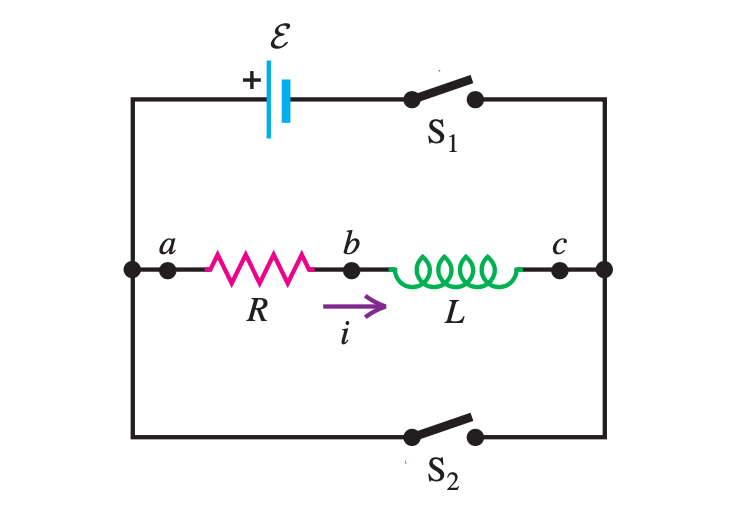
\includegraphics[scale=0.4]{fig/circuito2}
\caption{Al cerrar el interruptor $S_1$ se conecta la combinación $R-L $en serie con una fuente de fem $\varepsilon$. Al cerrar el interruptor $S_2$ al mismo tiempo que se abre $S_1$ se desconecta la combinación de la fuente.}
\end{figure}

Un circuito que incluye tanto un resistor como un inductor, y tal vez una fuente de fem, se llama circuito $R_L$ (figura \ref{fig:circuito2}).  El inductor ayuda a impedir los cambios rápidos en una corriente, lo que puede ser útil si se requiere una corriente estable y la fuente externa tiene una fem fluctuante.







%\end{document}

\end{document}

